
%\documentclass[12pt,a4paper]{report}
\documentclass[12pt,a4paper,openright, oneside, titlepage]{book} %,draft
%\linespread{1.5}
\usepackage{hyperref}							% Collegamenti ipertestuali
\hypersetup{
    bookmarks=true,         % show bookmarks bar?
    pdfnewwindow=true,      % links in new PDF window
    colorlinks=true,       % false: boxed links; true: colored links
    linkcolor=red,          % color of internal links (change box color with linkbordercolor)
    citecolor=blue,         % color of links to bibliography
    filecolor=magenta,      % color of file links
    urlcolor=cyan,          % color of external links
    urlbordercolor={1 1 1}% color of border around links
}
\usepackage[latin1]{inputenc}
\usepackage[english]{babel}
\usepackage{geometry}
\geometry{a4paper, inner=3cm, outer=2.5cm, top=2.5cm, bmargin=2.5cm}
\usepackage{amsmath}
\usepackage{amsfonts}
\usepackage{amssymb}
\usepackage{graphicx}
\graphicspath{ {figures/} }
\usepackage{verbatim}
\usepackage{textcomp}
\usepackage{xcolor}
\usepackage{makecell}
%\usepackage[sorting=none]{biblatex}
%\bibliography{bvitali_biblio}
\usepackage{rotating}


\usepackage{listings}
\lstset {
	language=C++,
	basicstyle=\footnotesize,
}
\usepackage[toc]{appendix}
\usepackage{float}
\usepackage{bm}

\usepackage[infront,standard, nowrite]{frontespizio}
\title{In situ monitoring\\ of the stopped muon flux at Mu2e\\\textbf{V\_0.9.1}}


%   Reduce the margin of the summary:
\def\changemargin#1#2{\list{}{\rightmargin#2\leftmargin#1}\item[]}
\let\endchangemargin=\endlist 

\begin{document}
%%%%%%%%%%% FRONT MATTER
\frontmatter
%\begin{comment}
	\begin{frontespizio}
	\Istituzione{University of Pisa}
	\Divisione{Department of Physics ``E. Ferm''}
	\Scuola{Master's Degree in Physics}
	\Logo [3.5cm]{cherubino_pant541}
	\Titolo {In situ monitoring of the stopped muon flux at Mu2e}
	\NCandidato{Candidate}
	\Candidato [517071]{Bastiano Vitali}
	\NRelatore{Thesis advisor}{Thesis advisor}
	\Relatore {Prof.~Simone Donati}
	\NCorrelatore{Research supervisor}{Research supervisor}
	\Correlatore{Dr.~Pavel Murat}

	\Piede{Academic Year 2019-2020}
	\end{frontespizio}
%\end{comment}
\maketitle

\chapter*{\centering Abstract}
\begin{changemargin}{1cm}{1cm}
The specific object of Mu2e search is  the neutrino-less coherent $\mu^-\rightarrow e^-$ conversion in the field of an aluminum nucleus and the signal is a monoenergetic electron of energy $ \approx 104.97$ MeV \cite{MTDR}.
%The parameter often used to indicate the strength of CLFV transition is the ratio $R_{\mu e}= (\mu^-N \rightarrow e^-N)/(\mu^-N \rightarrow \text{all } \mu \text{ captures})$ .
This process is forbidden in the Standard Model but allowed in many of its extensions: with minimal changes to include neutrino masses and oscillation, the Branching Ratio of this process, or the similarly interesting $\mu\rightarrow e \gamma$ decay, is expected to be of the order of $\mathcal{O}(10^{-54})$.
Values like these are below any currently achievable experimental sensitivity, and the observation of a signal would be unambiguous evidence of New Physics \cite{signorelli}.
The upper limit on the muon conversion was set by SINDRUM II at $7\times10^{-13}$ (90\% C.L.) \cite{SINDRUMII} and the goal of the Mu2e collaboration is an improvement of 4 order of magnitudes.\\
The Mu2e experiment can be conceptually divided in three stages: interaction of the primary proton pulse with the tungsten target and production of $\pi$ and $\mu$; collection and transport of the produced particles down to the aluminum stopping target; interaction with the stopping target and measurement of the output particles.
The measurement of the stopped muon flux is of cardinal importance for the normalization of the Mu2e results.
The baseline design includes two detectors developed to measure this flux, counting $\gamma$ emitted by the muonic atoms: HPGe and LaBr$_3$(Ce) \cite{STM:2016}\cite{LaBr3:2020}.
The studies performed by the Mu2e Collaboration show that these two systems can be reliably used to determine the overall normalization.\\
The number of stopped muons is proportional to the number of protons on target, which itself depends on the extraction system for the proton beam. 
The Mu2e beam delivery system will use a resonant extraction to create the proton pulses and this method is characterized by intensity fluctuations on the time scale of milliseconds \cite{SpillSim}. 
These fluctuations, aside from the proportional fluctuation of the number of muons, have a non trivial impact on the overall performance of the apparatus. 
For example, higher intensity proton bunches translate into higher veto rates by the Cosmic Rays Veto system, 
which is triggered by secondary particles generated by the proton interaction. 
Another example is the effect of the instantaneous luminosity on the reconstruction efficiency: higher intensity translates into higher detector occupancy, which in turn reduces the reconstruction efficiency.\\
The two cited detectors encounter limitations when trying to monitor the flux at the millisecond timescales: HPGe is by construction a slow detector while the rate of emission of the $\gamma (1809\textrm{ keV})$ the LaBr$_3$(Ce) will measure is too low.
As of today, no system allows to monitor these fluctuations and the goal of this Thesis is to try filling this gap.
The method we developed to monitor the fluctuations of the stopped muon flux, and by extension the fluctuation in the proton pulses intensity, is based on counting the number of muons captured in the stopping target by counting the number of protons produced in the process of the nuclear muon capture.
This is one of the possible processes a stopped muon can undergo and it can lead to the ejection of charged particles.\\
The reconstruction algorithms were developed by the Mu2e collaboration with the explicit (and sometimes implicit) aim to reconstruct tracks of electrons in an energy range of a conversion electron. 
The protons we are interested in behave quite differently from these electrons and the cardinal task of this study has been to tailor the reconstruction routines to these particles. 
This has been done by analyzing simulated events consisting of a single protons to optimize the procedure and understand the features of these tracks. 
A major difference with respect to the electrons is the non-relativistic nature of $100\div300$ MeV$/c$ protons: accounting for the low velocity is both a challenge and a unique signature of the tracks.\\
The use of a pulsed beam and the need to allow produced $\pi$ to decay and $\mu$ to interact in the stopping target forces the definition of a Mu2e \textit{event}: an event is comprised by everything which happens in a $1.7\ \mu$s window between the incidence two consecutive proton pulses.
This means that the reconstruction will be performed in an environment crowded by many different particles.
The next step of this study has been to estimate the performance of the method in a fully fledged Mu2e simulated event and to study what kind of selections would improve it.\\
Our results are satisfactory since the number of reconstructed protons is significant (few per event), and show that a monitor on the timescale of milliseconds is indeed possible.

\end{changemargin}

\tableofcontents
\listoffigures
\listoftables

%%%%%%%%%%% MAIN MATTER
\mainmatter
%---------------------%---------------------
%---------------------%---------------------
%---------------------
\chapter{Charged Lepton Flavour Violation}

{\itshape 
This Chapter provides a brief overview of the essential theoretical and experimental elements necessary to understand the goals of the Mu2e experiment at Fermilab and the work done for this Thesis. 
The purpose of the short introduction on the Standard Model and some of its extensions is to justify the interest to pursue experimental searches for Charged Lepton Flavour Violation. 
Since very exhaustive reviews of past, current and future experimental endeavours are already available in the literature (\cite{signorelli} \cite{bob_cflv}), only the most significant aspects of the muon-based experiments have been reviewed.} 

\section{The Standard Model}
Our current understanding of fundamental interactions is framed in the most predictive theory to date: the Standard Model (SM). 
This theory is based on the gauge symmetry group U$(1)_Y \times $SU$(2)_L\times $SU$(3)_C$.
The first two terms describe the electroweak interaction, $Y$ indicates the hypercharge and $L$ refers to the fact that this acts only on the left handed components of the fields. 
The last term describes the strong interaction and $C$ indicates the color charge.\\
The Standard Model contains 25 elementary fields, shown in Fig. \ref{_SM}: 
\begin{itemize}
\item 12 fermions are divided in two categories (6 leptons and 6 quarks) depending on the forces through which they interact.
Leptons do not interact through strong interaction and are subdivided in two groups based on the electric charge: charged ($e,\mu,\tau$) and neutral leptons ($\nu_e,\nu_\mu,\nu_\tau$). 
The labels show that these particles form doublets of flavour.
The 6 quarks are subject to all interactions and are divided depending on the electric charge ($u,c,t$ and $d,s,b$);
\item 12 bosons are the mediators of the interactions, $\gamma,Z,W^\pm$ for the electroweak interaction, and 8 gluons for the strong interaction;
\item The Higgs is a complex scalar weak isospin doublet that was introduced to justify the non-zero mass of the other particles and was recently discovered at LHC \cite{H:CMS}\cite{H:ATLAS}.
\end{itemize}

\begin{figure}[h!]
\centering
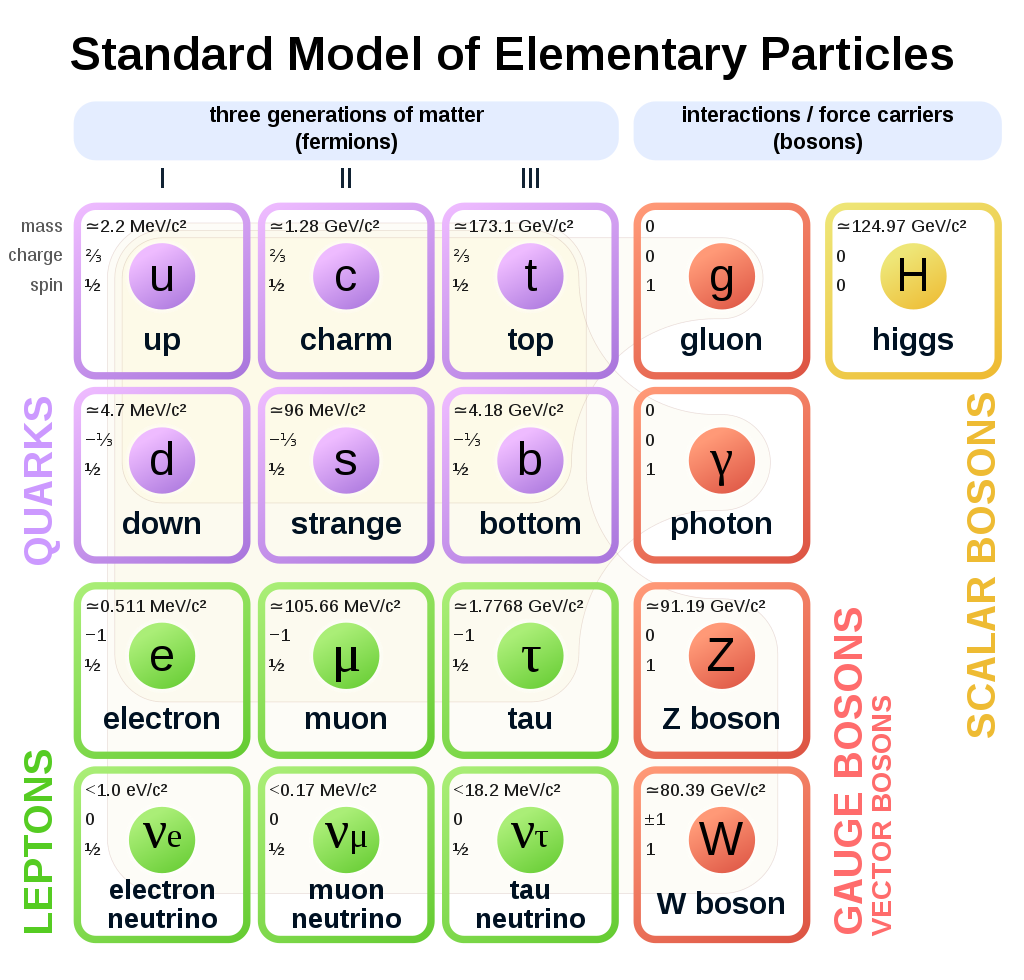
\includegraphics[width =0.6\textwidth, keepaspectratio]{SM}
\caption[Elementary particles of the Standard Model]{Elementary particles of the Standard Model. 
The colours help to identify the groups described in the text.}
\label{_SM}
\end{figure}

\subsection{Charged Lepton Flavour Violation}
Lepton Flavour conservation is accidental in the Standard Model and, until the observation of the neutrino oscillations  \cite{oscillations}, had been assumed valid. 
The discovery of neutrino oscillations showed that the eigenstates of the free particle and the weak  interaction are related through the non diagonal Pontecorvo-Maki-Nakagawa-Sakata matrix (PMNS).
At this point, the existence of  Lepton Flavor Violation was established and the rates could be obtained for this matrix.
The open question became if this violation is possible also in the charged lepton sector. 
In this framework, Charged Lepton Flavour Violation (CLFV) can be generated in specific processes, such as the $\mu\rightarrow e\gamma$ decay, or the neutrino-less coherent conversion $\mu^-N \rightarrow e^-N$, by loop diagrams involving neutrinos and the W boson (Fig. \ref{_feynman_SM}).
The estimates of the Branching Ratios of these processes are model dependent and well beyond the scope of this Thesis:  they can be found in the literature  \cite{signorelli}. \\
The interesting fact is that in many models CLFV-violating processes are suppressed by the sum of $(\Delta m_{ij}^2/M_W^2)^2$, where $\Delta m_{ij}^2$ is the mass-squared difference between neutrinos mass eigenstates. 
Since $\Delta m_{ij}$ is much smaller than $M_W$, the expected Branching Ratios are extremely low. 
For example, for the $\mu\rightarrow e\gamma$ decay, the prediction is $BR(\mu\rightarrow e\gamma)= 10^{-55}\div10^{-54}$ \cite {Petcov}. 
Physics processes with this probability are way below the sensitivity of the current or near-future experiments.
This means that any experimental evidence of CFLV would imply the existence of some missing piece in the extension of the lepton sector of the Standard Model.

\begin{figure}[h!]
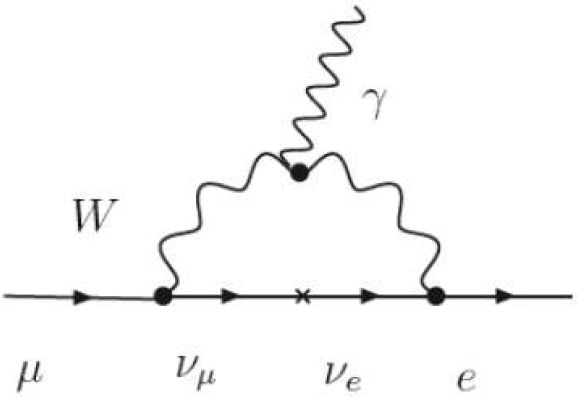
\includegraphics[scale=0.7]{feynman_mu-egamma}
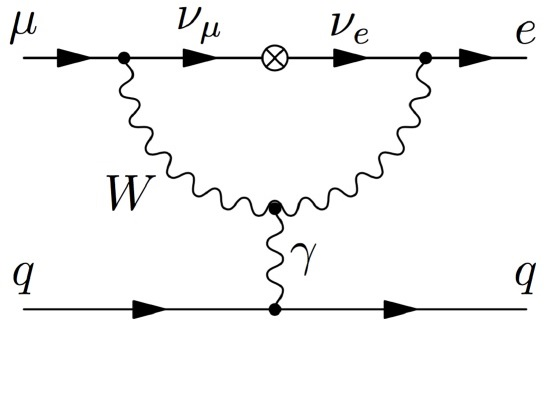
\includegraphics[scale=0.7]{feynman_mu2e}
\caption[Feynman: $\mu\rightarrow e\gamma$; $\mu^-N \rightarrow e^-N$]{Feynman diagrams contributing to the $\mu\rightarrow e\gamma$ decay (Left) 
and to the neutrino-less coherent conversion $\mu^-N \rightarrow e^-N$ (Right)
through neutrino oscillations.}
\label{_feynman_SM}
\end{figure}

\section{Beyond the Standard Model}
Although the Standard Model is a well-established and successful theory, there are still numerous open questions (dark matter, matter-antimatter asymmetry, the value of the Higgs mass and others) and many candidate extensions of the model have been proposed.
In our discussion we will briefly focus our attention on the super-simmetric CLFV.
Generally speaking, in SUSY models lepton and slepton (supersimmetric partners of the leptons) matrices are not aligned. 
In other terms, physical sleptons end up being mixtures of different flavours. 
In this context, CLFV arises from the interaction of Standard Model leptons and their SUSY partners (plus potential mixtures of other SUSY and Standard Model particles). 
In order to asses the rates for CLFV processes in SUSY models, it is necessary to know the masses of the particles appearing in the diagrams and the composition in flavour of the sleptons.
There are numerous flavour structures models: some are trivial (aligned leptons and sleptons mass matrices), while other are controlled by some flavour symmetry. 
The most known candidates for Grand Unified Theories (GUT) are based on SU(5) and SO(10) groups \cite{signorelli}.

\subsection{SUSY seesaw}
In this Section we will briefly describe the simplest mechanism that allows to include a neutrino mass term in the theory, following the example reported in \cite{Thomson}. 
In the Standard Model, this could be done by introducing a Dirac mass term:
$$\mathcal{L}_D=-\frac{1}{2}m_D(\overline{\nu}_L\nu_R+\overline{\nu}_R^c\nu_L^c) + h.c.$$
but this term would imply the existence of right-handed neutrinos (yet to be seen); also the fact that the mass has to be much smaller than for other fermions suggests that the solution should be searched for in an alternative way.
A different term that would satisfy the local gauge invariance is a Majorana mass term, formed by a $\nu_R$ and a $\bar{\nu_L}$, which trasforms as a singlet under the Standard Model gauge transformations:
$$\mathcal{L}_M=-\frac{1}{2} M(\overline{\nu}\vphantom{\nu}_R^c\nu_R+\overline{\nu}_R\nu_R^c)$$
Here the left-handed anti-neutrino appears as CP conjugate, which is $\nu_R^c$.
In this case, a coupling between particle and antiparticle is present, allowing $\nu$ to be its own antiparticle.\\
The general Lagrangian includes both Dirac and Majorana terms:
$$\mathcal{L}_{DM}= -\frac{1}{2}
\begin{pmatrix} 
\overline{\nu}_L & \overline{\nu}_R^c 
\end{pmatrix}
\begin{pmatrix} 
0 & m_D\\
m_D & M\\
\end{pmatrix}
\begin{pmatrix} 
\nu_L^c\\
\nu_R
\end{pmatrix} + h.c.$$
and, as always, the 'physical states' are the eigenstates of the mass matrix.\\
If the Majorana mass is taken to be much greater than the Dirac mass, the eigenvalues are:
$$
|m_\nu|\approx \frac{m_D^2}{M}\ ;\ m_N\approx M
$$
If the Majorana term exists, for each neutrino generation
this \textit{seesaw} mechanism would predict the existence of a very light particle (the one observed, $m_\nu\sim0.01$ eV) and a heavier counter-particle.
The eigenstates would be:
$$
\nu\approx (\nu_L+\nu_L^c)-\frac{m_D}{M}(\nu_R+\nu_R^c),\ \
N\approx (\nu_R+\nu_R^c)+\frac{m_D}{M}(\nu_L+\nu_L^c)
$$
leaving the light neutrinos couplings essentially the same as those of the Standard Model, while the heavy ones would be almost entirely right-handed and would not partecipate in weak charged or neutral currents.

\subsection{de Gouv\^{e}a}
A convenient general parameterization of SUSY models for CLFV-violating processes involving muons has been proposed by de Gouv\^{e}a \cite{deGouvea}:
\begin{align}
\mathcal{L}_{CLFV}=
\frac{m_\mu}{(\kappa+1)\Lambda^2}\overline{\mu}_R\sigma_{\mu\nu}e_LF^{\mu\nu}+
\frac{\kappa}{(\kappa+1)\Lambda^2}\overline{\mu}_L\gamma_\mu e_L (\overline{e}\gamma^\mu e)+h.c.
\label{eq_deGouvea}
\end{align}
In this expression, $m_\mu$ is the muon mass, $F^{\mu\nu}$ the photon field, $L$ and $R$ indicate the chirality of the fermion field.
On an intuitive level, the two terms correspond to 'dipole' and 'contact' 4-fermion interactions.
There are also two independent parameters,  $\Lambda$, the mass scale, and $\kappa$, which weights the two terms. 
Fig. \ref{_deGouvea} shows the relationship between the Branching Ratios of the processes $\mu\rightarrow e\gamma$, $\mu\rightarrow eee$ and $\mu N \rightarrow e N$ as a function of the parameter $\kappa$. 
%The parameter space for muon CLFV that has been excluded by previous experiments and the region that future experiments will be able to probe are also reported. 
%The upper limits expected at 90\% CL for the future experiments MEG upgrade, Mu3e, Mu2e and Mu2e at PIP II (Proton Improvement Plan-II) are also shown. 

\begin{figure}[h!]
\centering
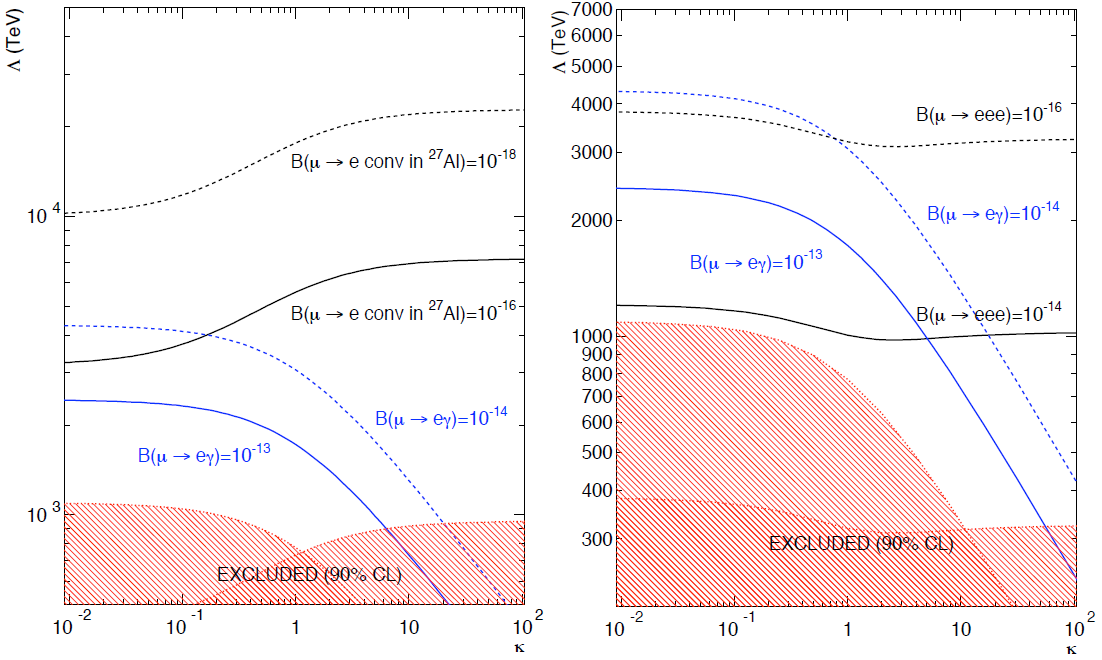
\includegraphics[width=0.9\textwidth]{deGouvea}
\caption[Limits on the BR]{Sensitivity of searches for $\mu\rightarrow e\gamma$, $\mu\rightarrow eee$ decays and $\mu N \rightarrow e N$ conversion in terms of the two parameters $\Lambda$ and $\kappa$. First parameter is the energy scale of the new interaction and the second one is the ratio between the four-fermion and loop interactions \cite{deGouvea}.}
\label{_deGouvea}
\end{figure}

\noindent A general conclusion on this (absolutely non exhaustive) introduction to SUSY could simply be that there are numerous fascinating models but, even within a specific model, there are no 'guaranteed' minimum rates to be expected. 
Due to the flexibility of these models, rates can be vanishing or exceed the current limits.
More experimental constraints are needed to reduce the plethora of available models.

\section{Phenomenology}
There are numerous physics processes which allow to pursue searches for Charged Lepton Flavour Violation:
\begin{itemize}
\item muon decays or conversions: 
$\mu\rightarrow e \gamma$, $\mu\rightarrow 3e$, $\mu^- N\rightarrow e^- N$, $\mu^- N\rightarrow e^+ N$; 
\item tau decays: $\tau\rightarrow \mu \gamma$, $\tau\rightarrow 3\mu$;
\item meson decays: $\pi^0\rightarrow \mu e$, $K_L^0\rightarrow\mu e$, $K_L^+\rightarrow \pi^+ \mu^+ e^-$;
\item Z decays like $Z^0\rightarrow\mu e$.
\end{itemize}
Physics processes involving muons have been thoroughly studied 
since low energy muon beams can be produced fairly easily 
at proton accelerator facilities and the final states can be precisely measured.\\
Before moving to the overview of the main experimental searches performed 
with muons, in the following we will provide a brief review 
of the relevant aspects of muon physics.

\subsection{The muon}
\label{muon}
The muon is a charged lepton discovered in 1937 by Anderson \cite{Anderson} 
and initially wrongly interpreted as the short-range strong force mediator predicted by Yukawa. 
After the study conducted by Conversi, Pancini and Piccioni \cite{ConvPancPicc}, 
the leptonic nature of the particle was established and the never-ending series of studies started 
with these two papers brought us to a deep knowledge of this particle. 
Today, the properties of the muon are well known and, in particular, the values for the mass and  mean lifetime are: 
$m_\mu = 105.6583745 \pm 0.0000024 $ MeV and $\tau =  2.1969811 \pm 0.0000022 \ \mu$s \cite{PDG}.
Muon decays almost exclusively as $\mu\rightarrow e\bar{\nu}_e\nu_{\mu}$ (table \ref{T_mu}) and the differential probability, in the reference frame of rest of the muon, is:

\begin{align}
\frac{d\Gamma(x,\vartheta)}{\mathrm dx \mathrm d\cos\vartheta}\approx \frac{G_F^2m_\mu^5}{192\pi^3}[(3-2x)\pm P\cos\vartheta(2x-1)]x^2
\label{eq_muon}
\end{align}
where $\frac{G_F^2m_\mu^5}{192\pi^3}=\frac{1}{\tau_\mu}$, $\vartheta$ is the direction of the electron momentum direction with respect to the muon spin, $x=2E/m_{\mu}$ is the reduced electron energy and $P$ is the polarization.\\
The spectrum in vacuum, known as Michel spectrum, is the same for both signs of the electrical charge and, aside for radiative corrections (due to the emission of an additional $\gamma$), has a kinematic endpoint at around half of the muon mass (Fig. \ref{_Michel}).\\

\begin{figure}[h!]
\centering
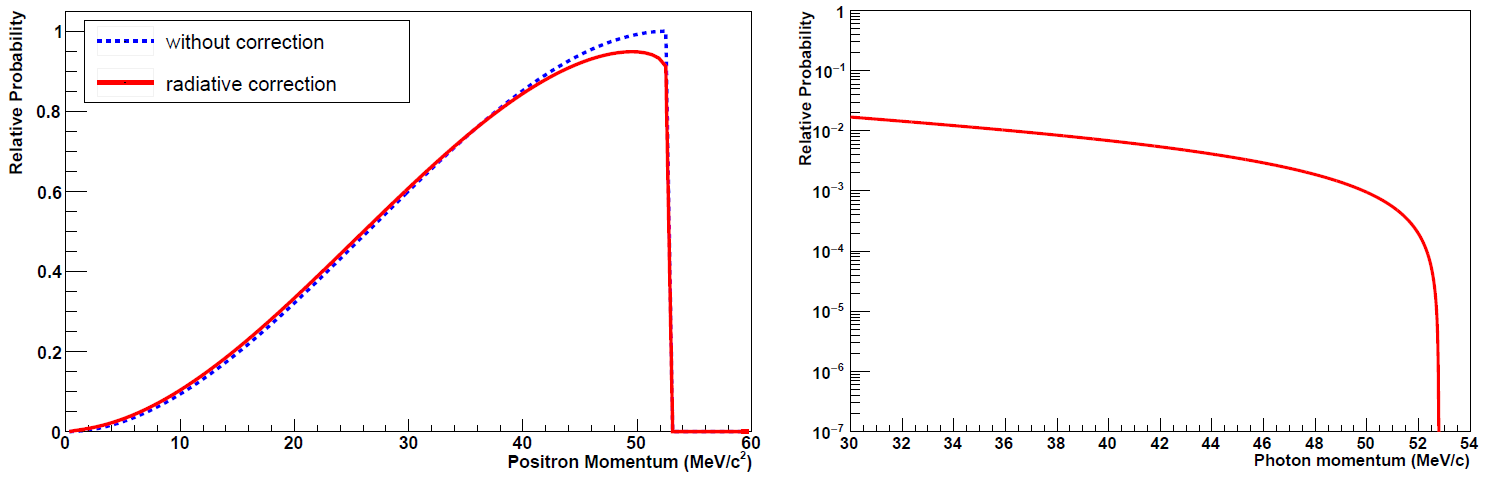
\includegraphics[scale=0.5]{Michel}
\caption[Michel spectrum]{Michel spectrum before and after the radiative corrections \cite{signorelli}. The plot on the right is a particular of the end point in log scale, this helps to understand how quickly the spectrum goes to zero.}
\label{_Michel}
\end{figure}

\begin{table}
\centering
\begin{tabular}{|c|c|c|}
\hline
Decay channel & BR & CL\\
\hline
\hline
$\mu^- \rightarrow e^-\overline{\nu}_e\nu_\mu$&$\sim100\%$&\\
$\mu^- \rightarrow e^-\overline{\nu}_e\nu_\mu e^-e^+$&
$(3.4\pm0.4)\times10^{-5}$&\\
\hline
$\mu^- \rightarrow e^-\nu_e\overline{\nu}_\mu$&$<1.2\%$&$90\%$\\
$\mu^+ \rightarrow e^+\gamma$&$<4.2\times10^{-13}$&$90\%$\\
$\mu^- \rightarrow e^-e^+e^-$&$<1.0\times10^{-12}$&$90\%$\\
$\mu^- \rightarrow e^-2\gamma$&$<7.2\times10^{-11}$&$90\%$\\
\hline
\end{tabular}
\caption[Muon decay channels]{Muon decay channels \cite{PDG}.}
\label{T_mu}
\end{table}

\subsubsection{Stopped muons}
\label{stopped_muon}
As we have just mentioned, 
the lifetime of a free moving muon is $\tau\approx 2.2\ \mu$s. 
When a $\mu^-$ is stopped in matter, 
it displaces an electron and sets in the lowest energy orbit at a radius that depends on the nucleus $Z$. 
Once the muon is in the orbit, it can either decay with probability $\Lambda_d$ 
or be captured by the nucleus with probability $\Lambda_c$. 
The lifetime of this system is then:
\begin{align}
\frac{1}{\tau}=\Lambda_d + \Lambda_c \label{eq_tau}
\end{align}
The capture probability increases rapidly: 
for example, for $Z\sim 11$ it is approximately equal to the decay probability $\approx 4.5 \times 10^5$ s$^{-1}$,
 while for higher $Z$ it scales as $Z^4$.
The consequence of the increased $\Lambda_c$ is that the effective lifetime is reduced 
as a function of the atomic number $Z$: 2 $\mu$s for carbon; 
880 ns for aluminum; 
330 ns for titanium; 
73 ns for gold.\\
On top of the lifetime variation, 
the presence of the nucleus opens a number of possible scenarios for interaction. 
We will discuss this point extensively later but for now it is sufficient to say 
that the interaction with the nucleus can also generate a long tail in the energy spectrum 
of the electron coming from the muon decay, up to $E_e\approx m_\mu -B -E_R$. In this equation $B$ is the binding energy of the muonic atom and $E_R$ is the recoil of the nucleus. 
These electrons are often referred to as Decay In Orbit (DIO) and their spectrum, 
which is obviously $Z$-dependent, is shown in Fig \ref{_DIO_pre}.\\

\begin{figure}[h!]
\centering
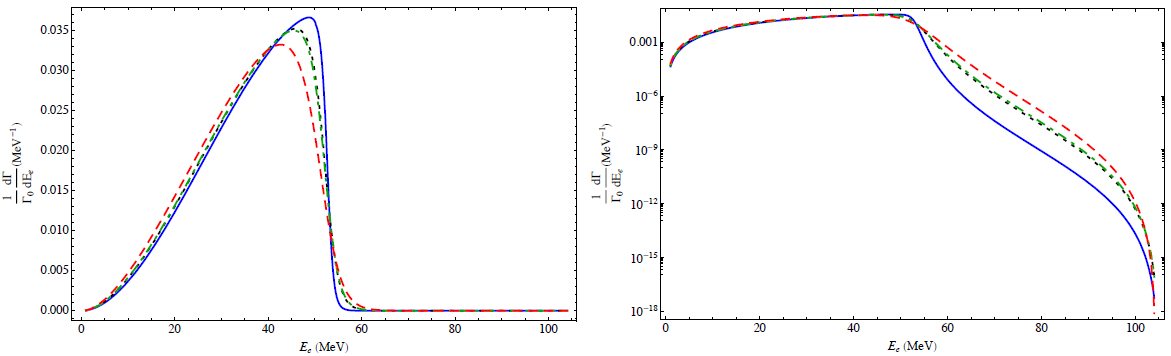
\includegraphics[scale=0.8]{DIO_materials}
\caption[Decay In Orbit spectra]{Electron spectrum in different materials, normalized to the free-muon decay rate \cite{signorelli}. The solid blue line is for carbon, the black dotted line for aluminum, the green dot-dashed line for silicon and the red dashed line for titanium.}
\label{_DIO_pre}
\end{figure}

\subsection{Motion of a charged particle in magnetic field}
\label{magnets}
The motion of a charged particle through a magnetic field is well known known phenomenon, 
rigorously explained in many textbooks. The basic principle is the Lorentz force:
$$\textbf{F}=q\textbf{v}\times\textbf{B}$$
A charge particle moving in a uniform solenoidal field describes the combination of free trajectory 
and a circular motion, namely a helix, with the property:
\begin{align}
|\textbf{B}|\rho = \frac{p_\perp}{|q|} 
\label{eq_brho}
\end{align}
This is the simplest situation but more complex magnetic fields can generate very interesting and useful motions; 
here we will discuss the use of a gradient to accelerate particles 
and the perpendicular drift of the particles in a curved magnetic field.\\
A magnetic field with a non null gradient varies in intensity as a function of the position. 
The force generated by the gradient is proportional to the magnetic momentum $\mu$ 
(the $E$ in the definition is the energy) of the particle and can be expressed as:
\begin{align}
\textbf{F} &= -\mu \nabla \textbf{B} \\
\mu &= \frac{c^2 p_\perp^2}{2EB}
\end{align}
This force does not change the particle energy but changes the direction of the momentum and, 
if the gradient is strong enough, it is possible to flip the direction of motion, 
effectively reflecting the particle with a \textit{magnetic mirror}. 
More complex gradients can be even used to trap a particle in a specific region 
or, conversely, to assure no particle stays in the same region for too long 
(for example to avoid the blinding of a detector).\\
The other interesting property is connected to the use of curved magnetic fields. 
In a curved solenoid it is possible to show that 
the particle orbit point drifts in the direction perpendicular to the bending plane. 
The drift is characterized by a drift velocity $v_D$ (eq. \ref{eq_vd}) 
and it is possible to evaluate the total drift $D$ (eq. \ref{eq_D}) 
as a function of the path along the curved solenoid $S$:
\begin{align}
v_D&=\frac{m\gamma c}{eBR}\left(v^2_\parallel+\frac{1}{2}v^2_\perp\right) \label{eq_vd}  \\
D&\propto pS\left(\frac{1}{\cos \vartheta}  + \cos \vartheta \right) \label{eq_D}
\end{align}
In the above equations, parallel and perpendicular refer to the magnetic field and R is the bending radius of the solenoid. 
On the other hand, $\vartheta$ is the pitch angle of the helix from the magnetic field axis 
and the sign of the drift depends on the sign of the charge: 
this characteristics can be used to separate particle of different charges using a curved solenoid.

\subsection{Single event sensitivity}
When searching for an extremely rare physics process, 
or trying to set an upper limit on its probability, 
is often useful to estimate the probability of spectating one event 
under the tested hypothesis 
(which depends on the process, the background in the window used for the measurement 
and the apparatus performance). 
Assuming a given probability for the process under study, 
this \textit{single event sensitivity} ($SES$) is connected to the total number of expected events as follows:
\begin{align*}
N_{events} = \frac{BR_{process}}{SES}
\end{align*}
The estimate of the $SES$ is all but trivial 
and what is often cited as \textit{sensitivity} is actually $2.3\times SES$. 
This value is the consequence of assuming a poissonian distribution 
for the number of events (the bayasian 90\% upper limit for a 0 extraction from a poisson distribution is 2.3).\\

\section{CLFV experimental searches with muons}
Searches for violations in the leptonic sector have been pursued for decades, 
beginning in 1947 \cite{ConvPancPicc} with the study of the decay of the neo-discovered muon \cite{Anderson}.
This Section will report a brief summary and description 
of the key searches for CLFV and table \ref{T_CLFV} shows the experimental limits 
(with relative process and some references). 
We will focus on the searches using leptons: 
this history is reported in  Fig. \ref{timeline_measures}. 
Even more specifically, our interest is focussed on the processes involving muons 
(Table \ref{T_CLFV_mu}): $\mu\rightarrow e\gamma$, $\mu N\rightarrow e N$, and $\mu\rightarrow 3e$.
Fig. \ref{_timeline_future} shows the time-line of the present and future dedicated experiments,
including MEG-II at the Paul Scherrer Institut (Switzerland), COMET at J-PARC (Japan),
and Mu2e at Fermilab (United States).

\begin{figure}[h!]
\centering
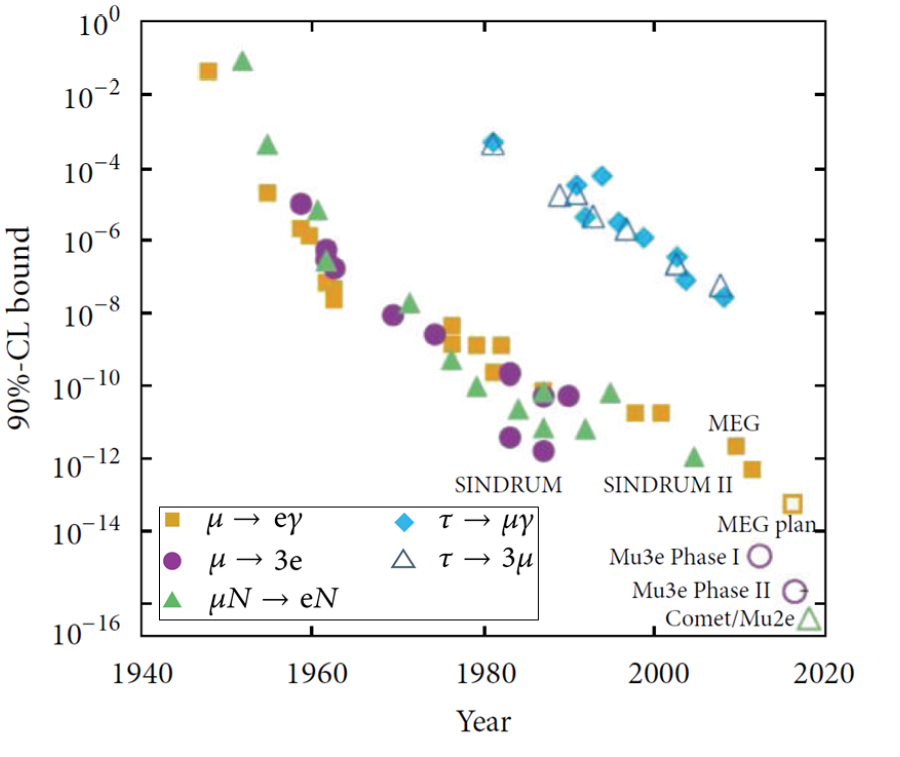
\includegraphics[scale=0.7]{timeline_measures}
\caption[History of CLFV searches]{Summary of the experimental searches for CLFV processes as a function of the years \cite{Chiappini}.}
\label{timeline_measures}
\end{figure}

\begin{figure}[h!]
\centering
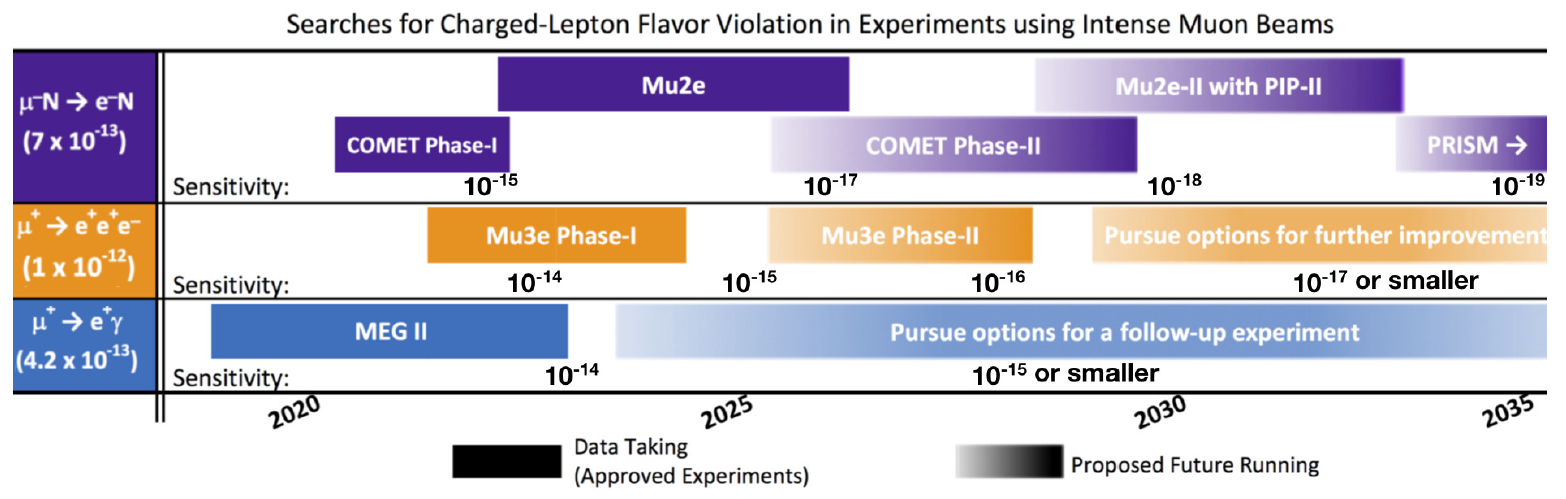
\includegraphics[scale=0.5]{timeline_future}
\caption[Experiments schedules]{Planned data taking schedules for current experiments and possible schedules for future proposed upgrades \cite{Baldini:2019}. The current best limits for each process are shown on the left, 
while expected future sensitivities are indicated by orders of magnitude along the bottom of each row.}
\label{_timeline_future}
\end{figure}

\begin{table}[!h]
\centering
\begin{tabular}{c|c|c}
\hline
Process & Upper limit & reference\\
\hline
\hline
$\mu^+\rightarrow e^+\gamma$ & $5.7\times 10^{-13}$ & \cite{MEG}\\
$\mu^+\rightarrow e^+e^+e^-$ & $1.0\times 10^{-12}$ & \cite{SINDRUM}\\
$\mu^-$Ti$\rightarrow e^-$Ti  & $1.7\times 10^{-12}$ & \cite{SINDRUM}\\
$\mu^-$Au$\rightarrow e^-$Au  & $7\times 10^{-13}$   & \cite{Bertl}\\
$\mu^+e^-\rightarrow \mu^-e^+$ & $8.3\times 10^{-11}$ & \cite{Willmann}\\
$\tau^\pm\rightarrow e^\pm\gamma$ & $3.3\times 10^{-8}$ & \cite{Aubert}\\
$\tau^\pm\rightarrow \mu^\pm\gamma$ & $4.4\times 10^{-8}$ & \cite{Aubert}\\
$\tau^-\rightarrow e^-e^-e^+$ & $2.7\times 10^{-8}$ & \cite{Hayasaka}\\
$\tau^-\rightarrow \mu^-\mu^-\mu^+$ & $2.1\times 10^{-8}$ & \cite{Hayasaka}\\
$\tau^-\rightarrow e^-\mu^-\mu^+$ & $2.7\times 10^{-8}$ & \cite{Hayasaka}\\
$\tau^-\rightarrow \mu-e^-e^+$ & $1.8\times 10^{-8}$ & \cite{Hayasaka}\\
$\tau^-\rightarrow e^+\mu^-\mu^-$ & $1.7\times 10^{-8}$ & \cite{Hayasaka}\\
$\tau^-\rightarrow \mu+e^-e^-$ & $1.5\times 10^{-8}$ & \cite{Hayasaka}\\
$\pi^0\rightarrow \mu e$ & $3.6\times 10^{-10}$ & \cite{Abouzaid}\\
$K^0_L\rightarrow \mu e$ & $4.7\times 10^{-12}$ & \cite{Ambrose}\\
$K^+\rightarrow \pi^+\mu^+e^-$ & $1.3\times 10^{-11}$ & \cite{Sher}\\
$K^0_L\rightarrow \pi^0\mu^+e^-$ & $4.4\times 10^{-10}$ & \cite{Abouzaid}\\
$Z^0\rightarrow \mu e$ & $7.5\times10^{-7}$& \cite{Aad}\\
$Z^0\rightarrow \tau e$ & $9.8\times10^{-6}$& \cite{Akers} \\
$Z^0\rightarrow \tau \mu$ & $1.2\times10^{-6}$& \cite{Akers}\\
\hline
\end{tabular}
\caption[Limits for CLFV processes]{Experimental upper limits for a variety of CLFV processes.}
\label{T_CLFV}
\end{table}

\begin{table}[!h]
\centering
\begin{tabular}{|c||c|c|c|}
\hline
& $\mu^+\rightarrow e^+\gamma$ & $\mu^+\rightarrow e^+e^-e^+$ & $\mu^- N \rightarrow e^- N$ \\
\hline \hline 
Background &
Accidental &
Radiative muon decay &
Decay in orbit \\
\hline
Beam &
Continuous &
Continuous &
Pulsed \\
\hline
Current limit &
\makecell{$4.2 \times 10^{-12}$ \\ MEG \cite{MEG}} &
\makecell{$1\times10^{-12}$ \\ SINDRUM \cite{SINDRUM}} & 
\makecell{$7\times10^{-13}$ \\ SINDRUM II \cite{SINDRUMII}} \\
\hline
Planned experiment &
\makecell{MEG II \\ PSI \cite{MEG_upgrade}\cite{MEG_II}\cite{Papa}}&
\makecell{Mu3e \\ PSI \cite{Mu3e:2014}\cite{Mu3e:2016}\cite{Papa}} &
\makecell{Mu2e \\ FNAL \cite{mu2e_proposal} \cite{MTDR}\\ COMET \\ JPARC\cite{COMET_2009}\cite{COMET_2012}\cite{COMET_2012_2}\cite{COMET_I}} \\
\hline
Planned sensitivity &
$\sim 6\times 10^{-16}$&
$\sim 10^{-16}$&
$\sim$ few $\times 10^{-17}$ \\
\hline
\end{tabular}
\caption[CLFV searches with muons]{Overview of muon CLFV experiments}
\label{T_CLFV_mu}
\end{table}

\noindent Due to obvious space limitations, it is not possible
to dedicate a section to each important experiment related to this very prolific field of study. 
In this spirit, we will nominate and give references to some of the experiments that played a central role. \\
Crystalbox \cite{Crystalbox:1984} \cite{Crystalbox:1988} was arguably the first 'modern' $\mu\rightarrow e\gamma$ experiment. With its successor MEGA \cite{MEGA:1999} \cite{MEGA:2002} was an important step in the study of the $\mu^+\rightarrow e^+\gamma$ channel. SINDRUM \cite{SINDRUM} and SINDRUM II \cite{SINDRUMII}, 
both performed at the Paul Scherrer Institute, set the current wrold-best limits r
espectively on the $\mu \rightarrow 3 e$ and $\mu^-\rightarrow e^- N$. 
We will only describe the apparatus for SINDRUM II, in one of the following Sections, 
because it set the limit on the process $\mu N \rightarrow e N$ object of Mu2e search.\\
The overview of the experimental scenario as of today will be given by physical process.

\begin{comment}
\begin{itemize}
\item Crystalbox \cite{Crystalbox:1984} \cite{Crystalbox:1988} was arguably the first 'modern' $\mu\rightarrow e\gamma$ experiment. It used a pulsed 800 MeV proton beam, the electron was tracked while the photon was detected with a Na(Ti) calorimeter: $\sim400$ Na(Ti) crystals surrounding a cylindrical drift chamber and plastic scintillation counters with no magnetic field. The upper limit achieved was $\Gamma(\mu^+\rightarrow e^+\gamma)/\Gamma(\mu^+\rightarrow e^+ \nu \overline{\nu})<4.9\times 10^{-11}$.
\item MEGA \cite{MEGA:1999} \cite{MEGA:2002}, like the previous experiment, was performed at Los Alamos. The cylindrical structure was kept and the apparatus was formed by an inner chamber, surrounding the stopping target, and seven smaller cylindrical chambers surrounding it (sometimes indicated as \textit{Snow White} ad \textit{Seven Dwarves} \cite{bob_cflv}). The limit set by this experiment was $1.2\times10^{-11}$ and the relatively poor improvement from its predecessor was mainly related to the reduced duty factor due to the pile-up.
\item SINDRUM \cite{SINDRUM} and SINDRUM II \cite{SINDRUMII} at were performed at the Paul Scherrer Institute. We will only describe the apparatus for SINDRUM II, in a following section, because it set the limit on the process Mu2e is going to test.
\item TRIUMF
\end{itemize}
\end{comment}

\subsection{Search for the $\mu^+ \rightarrow e^+ \gamma$ decay}
The most convenient experimental technique to search for the $\mu^+ \rightarrow e^+ \gamma$ decay
is to have the $\mu^+$ decay at rest. In this case, the signal  
signature is a back-to-back positron and photon pair, with $E_e=E_\gamma\approx 52.8$ MeV. 
There are two most significant sources of background: 
the prompt background due to the \textit{radiative muon decay} 
($\mu^+\rightarrow e^+ \nu_e \overline{\nu}_\mu\gamma$) 
and the accidental coincidence of $\mu^+\rightarrow e^+ \nu_e \overline{\nu}_\mu$ 
with a random $\gamma$ generated by annihilation or bremsstrahlung.
The accidental background is dominant and proportional to the instantaneous muon rate. 
Since the experimental sensitivity is proportional to the total number of stopped muons, 
a continuous beam is preferred.
The current best limit  BR$(\mu^+\rightarrow e^+\gamma)<4.2\times10^{-13}$ 
was set by the MEG experiment at the Paul Scherrer Institut\cite{MEG}.

\subsubsection{The MEG experiment at Paul Scherrer Institut}
The MEG experiment \cite{MEG} has been designed around two concepts: 
exploiting a liquid xenon detector (LXe) for positron and photon tracking and an anti-bottle magnetic field. 
Muons are stopped in a polyethylene target in the center of the magnet. Positron momentum is measured by a combination of drift chambers (DCH) and plastic scintillator timing counters (TC). 
On the other hand, the photon energy and direction are measured in a volume of liquid xenon with more than 800 photo-multipliers tubes.\\
The measured quantities are the electron and photon energies ($E_e$ and $E_\gamma$) and the relative positions (angles $\vartheta_{e\gamma}$, $\varphi_{e\gamma}$ and time $t_{e\gamma}$). 
The resolutions are dictated by the need of effectively separate the background, like the radiative muon decays. 
The requirements translate into an energy resolution of $\lessapprox 1\%$ for both particles.\\
If MEG had adopted a uniform magnetic field, positrons emitted at low pitch angle would end up passing many times through the tracker and would blind it. In MEG the magnetic field decreases symmetrically from the center towards the periphery to push the particles away from the center. The exact shape of the field has been chosen to have a track radius proportional to the \textit{absolute} momentum instead of the transverse. 
This allows to discard low energy positrons by simply placing the detector at sufficient distance from the magnet axis. 
This feature is a specific of the MEG magnetic system and justifies its name as ``COnstant Bending RAdius'' (COBRA) magnets.\\
The DCH spectrometer is made of 16 trapezoidal drift chambers, arranged radially and filled with He-C$_2$H$_6$. The radial coordinate is evaluated using the timing registered by the DCH and the TC while the $z$ position is determined by measuring the induced charged on the zig-zag shaped pads on the side of the drift chambers. The momentum resolution for the positron is $\approx330$ keV.\\
The choice of using a liquid xenon scintillating detector for the photon reconstruction was driven by the need to minimize
the amount of passive material in the detector\footnote{A detector comprised by crystals is bound to have passive material at the surface of each crystal.} and have an excellent time resolution. 
This choice provides a higher light yield than, for example, a NaI crystal and a much shorter decay time: 
the timing resolution on the measurement photon interaction time is below 100 ps.\\
MEG collected $7.5\times10^{14}$ stopped muons in the years 2008-2013 
and, as already mentioned, 
set the currently world-best a limit of BR$(\mu^+\rightarrow e^+\gamma)<4.2\times10^{-13}$ at 90\% CL \cite{MEG}.

\begin{figure}[h!]
\centering
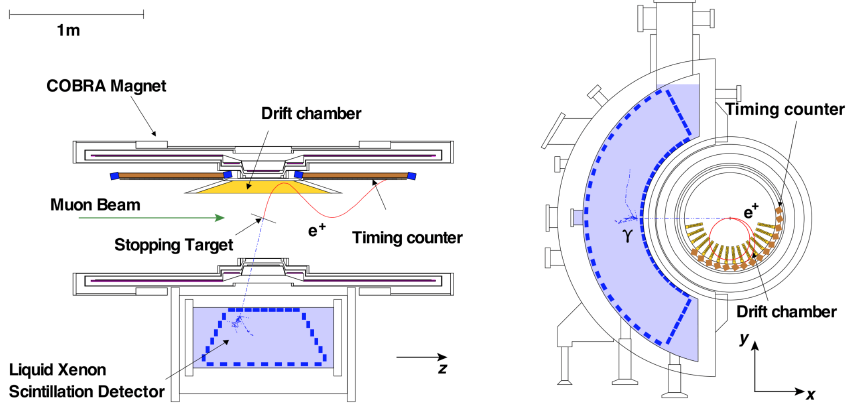
\includegraphics[scale=1]{MEG}
\caption[MEG experiment]{Pictorial view of the MEG experiment \cite{Chiappini}\cite{MEG}.}
\label{_MEG}
\end{figure}

\subsubsection{The upgraded MEG II experiment} 

\noindent
The upgraded MEG II experiment was proposed to reduce the contamination due to the accidental background 
that could not be further reduced in MEG \cite{MEG_upgrade} \cite{MEG_II}.
In the following, we have reported the list of the most significant upgrades of the infrastructure and experiment:

\begin{itemize}
\item Increase the muon flux to $7\times10^7\ \mu^+/$s;
\item Install a thinner but more inclined stopping target to reduce the multiple scattering and bremsstrahlung 
while keeping the same stopping power ($205 \rightarrow 140\ \mu$m);
\item Replace the drift chamber with a new cylindrical drift chamber (CDCH) designed  
to have higher granularity and transparency and made of 9 layers of drift cells to improve positron track reconstruction; 
\item Replace the plastic scintillator timing counters (TC) with a more segmented system (pixellated-TC);
\item Change the type (partially) and distribution of the photo-sensors to improve reconstruction;
\item Introduce a Radiative Decay Counter: a target of plastic scintillator and LYSO calorimeter positioned transversely to detect positron from RMD emitted at low angle.
\end{itemize}
The goal of the MEG II apparatus is to further reduce the limit on the Branching Ratio to the level of BR$(\mu^+\rightarrow e^+\gamma)<5\times10^{-14}$ in three years of data taking. 
The engineering runs for MEG II detectors commissioning are currently ongoing.

\begin{figure}[h!]
\centering
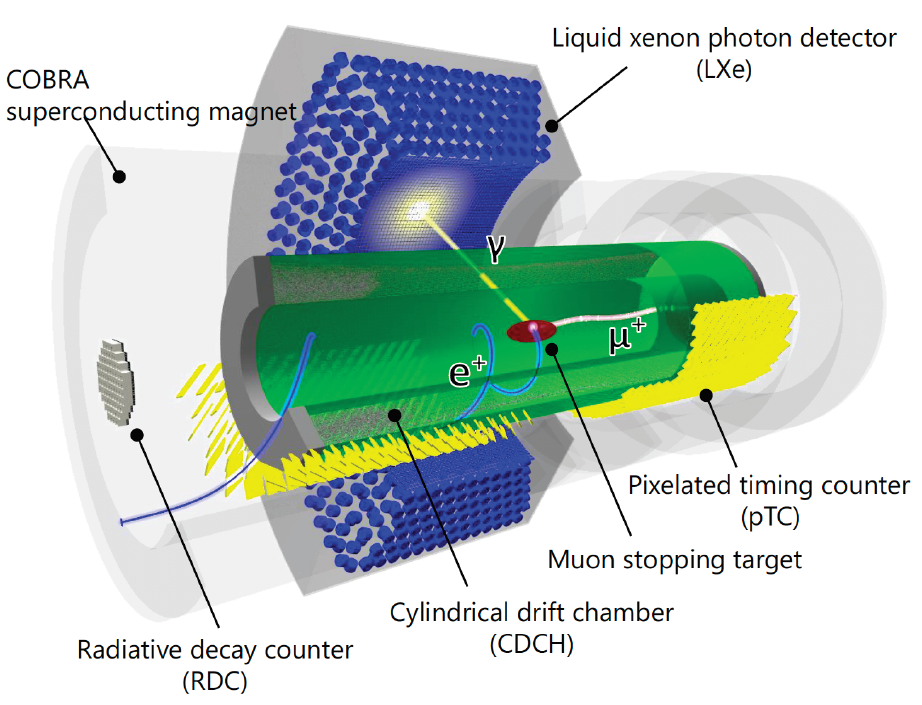
\includegraphics[scale=0.8]{MEG_II}
\caption[MEG II experiment]{Pictorial view of the MEG II experiment \cite{MEG_II}.}
\label{_MEG_II}
\end{figure}

\subsection{Search for the $\mu^+ \rightarrow e^+ e^+e^-$ decay}
The signature of the $\mu^+$ decay at rest is two positrons and one electron in a time coincidence, 
with total energy equal to the muon mass and null vector sum of the particle momenta.
Since this is a three-body decay and particles may have a momentum in a range between
few MeV and half the muon mass, a thin and low-mass tracker with an excellent resolution is necessary.
It is also important to estimate the probability of having the three particles with momenta above the detector threshold.
A prompt source of background for this search is due to the allowed 
$\mu^+\rightarrow e^+e^-e^+\overline{\nu}_{\mu}\nu_e$ (radiative decay with internal conversion) 
which has a BR$\approx 3.4\times 10^{-5}$ 
and becomes indistinguishable from the signal when the neutrinos have very low energy. \\
The other most significant background is due to the coincidence of one Michel decay 
with a $e^+e^-$ pair (1-MD) or two Michel decays with a single $e^-$ (2-MD). 
In this case, the $e^+e^-$ pair can be produced by Bhabha scattering or photon conversion, 
while the $e^+$ can be produced by Compton scattering or mis-reconstructed $e^+$ and $e^+e^-$ (with the $e^-$ not reconstructed). Clearly, this source of background depends on the muon rate and can be suppressed 
with precise vertex reconstruction, timing and track reconstruction.
As for $\mu^+ \rightarrow e^+ \gamma$, the use of a continuous beam is favorable.\\
Currently the world-best limit on this decay is BR$(\mu^+ \rightarrow e^+ e^+e^-)<10^{-12}$ 
and was set by the experiment SINDRUM in 1988 \cite{SINDRUM}.\\
To be competitive with the $\mu^+\rightarrow e^+\gamma$ search, 
an improvement of $10^4$ is needed: 
if the running time is $\mathcal{O}($years$)\sim 3\times 10^7$ s, 
then a beam with the intensity of $10^9\ \mu^+/$s is necessary.

\subsubsection{The Mu3e experiment at Paul Scherrer Institut}
The goal of the Mu3e experiment is to achieve a single-event-sensitivity of  the order of $10^{-16}$
on the $\mu^+ \rightarrow e^+ e^+e^-$ decay \cite{Mu3e:2016}.  
This experiment will use the same muon beam as MEG II and will stop muons on a thin hollow double-come Mylar target. 
The detector will be a 2 m cylinder placed inside a 1.5 T magnetic field and segmented in 5 sections (Fig. \ref{_Mu3e}). 
The central station will consist of two double layers of pixel detectors and a scintillating fiber tracker. 
The other four stations will be made of two layers of pixel sensors and a hodoscope of scintillator. 
A pictorial view of the Mu3e apparatus is reported in Fig. \ref{_Mu3e_3D}.\\
Since the Mu3e search relies heavily on accurate track reconstruction, 
multiple Coulomb scattering is a limiting factor and the technical choices adopted for the detector design
have been taken to minimize this effect. 
The tracker consists of High Voltage Monolithic Active Pixel (HV-MAPS) 
and the design is such as to exploit the (partial) canceling of the multiple scattering in half of turn. 
The estimated time and vertex resolutions are $\sigma_t\approx 100$ ps  and $\sigma_{xy}\approx 200\ \mu$m; 
the momentum resolution is $100\div400$ keV for $10\div53$ MeV/c particles \cite{signorelli}.\\
The experiment is projected in three phases  \cite{signorelli}, shown in Fig. \ref{_Mu3e}:
\begin{itemize}
\item Phase Ia: beam with an intensity of $\mathcal{O}(10^7)\ \mu^+/$s and only the tracker installed;
\item Phase Ib: beam with an intensity of $\mathcal{O}(10^8)\ \mu^+/$s (max at present for PSI) 
with the addition of the scintillating fibers and two of the additional tracking stations;
\item Phase II: beam with an intensity at $\mathcal{O}(10^9)\ \mu^+/$s (new beam-line needed) 
with the addition of the other two stations to reach the single-event-sensitivity of $10^{-16}$.
\end{itemize}

\begin{figure}[h!]
\centering
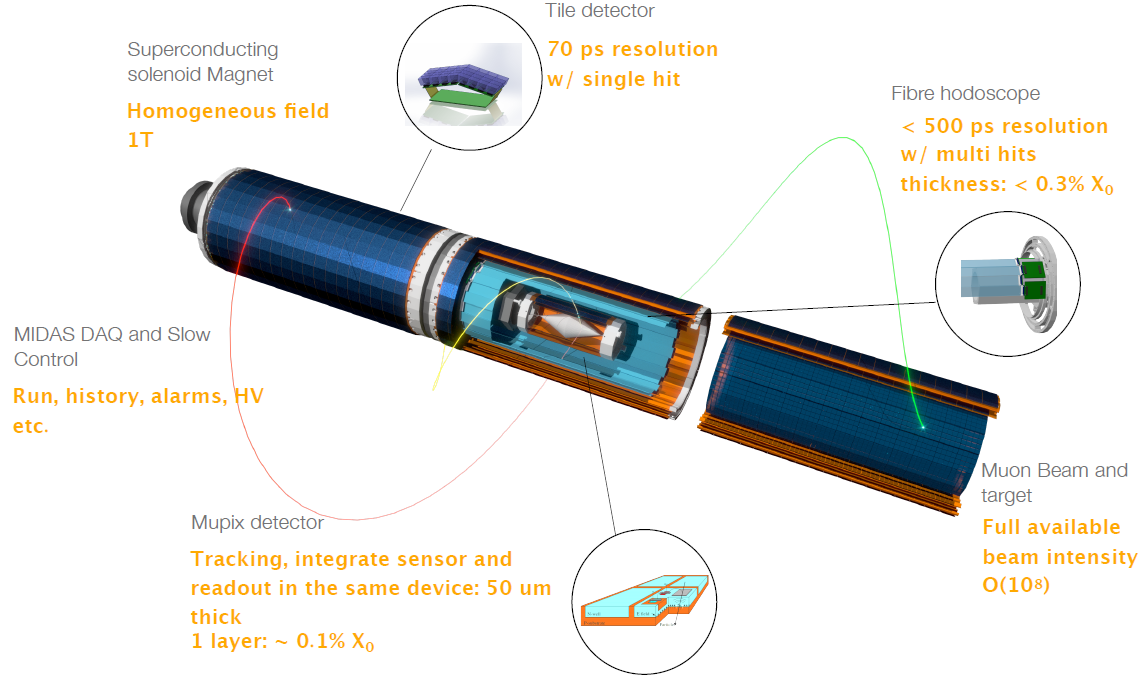
\includegraphics[scale=0.6]{Mu3e_3D}
\caption[Mu3e experiment]{Pictorial view of the Mu3e apparatus \cite{Papa}.}
\label{_Mu3e_3D}
\end{figure}

\begin{figure}[h!]
\centering
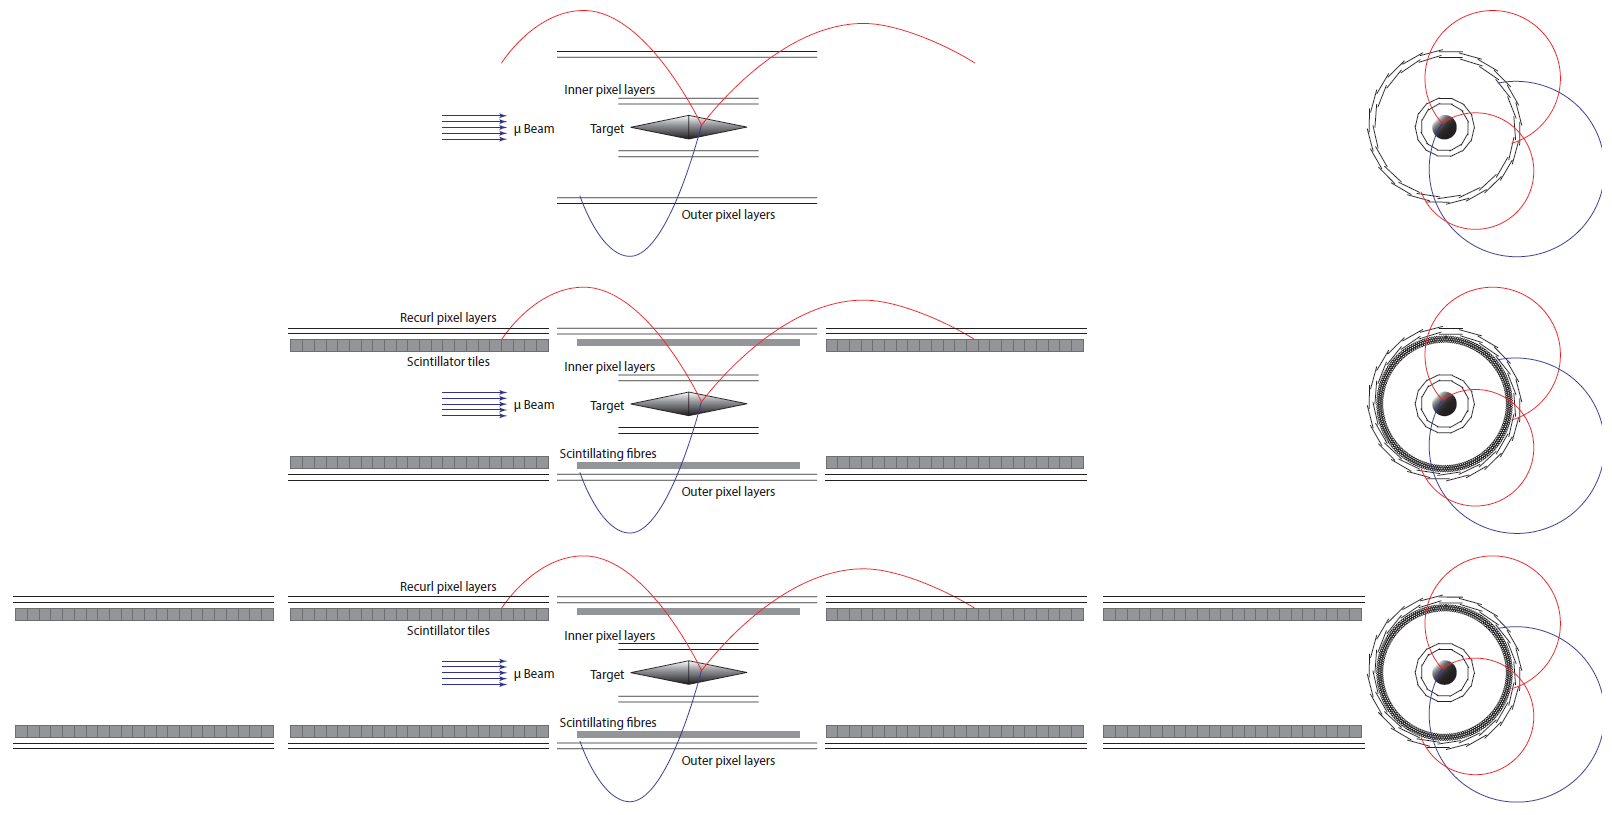
\includegraphics[scale=0.5]{Mu3e}
\caption[Mu3e experiment phases]{A sketch view of the Mu3e apparatus \cite{Mu3e:2013} and the various phases.}
\label{_Mu3e}
\end{figure}



\subsection{Search for the muon-to-electron conversion ($\mu^-N \rightarrow e^-N$)}
\label{muNeN}
In the neutrino-less coherent conversion, all the muon energy goes to the electron since the amount of energy
transferred to the nucleus recoil is almost negligible. The signal signature is thus a monochromatic 105 MeV electron.
The main advantage of the conversion search with respect to the $\mu\rightarrow e\gamma$ search is the
larger momentum and better separation of the electron signal from the background.
In a ``doughnut-shaped'' experiment, the level of background due to low momentum particles
can thus be reduced to a manageable level.

\noindent
In order to cancel the uncertainty due to the overlap of the nucleus and the muon wave functions, 
the quantity to be measured is: 
$$R_{\mu e} = \frac{\Gamma(\mu\rightarrow e)}{\Gamma(\textrm{muon capture})}$$
Since no coincidence is required, the experiment relies heavily on the electron reconstruction. 
The primary sources of background are:
\begin{itemize}
\item Electrons produced by the muon decay in orbit (DIO), which have a long tail that can contaminate the signal region;
\item High energy photons produced by radiative captures of pions (RPC) and muons (RMC) that can convert asymmetrically
and generate electrons in the signal energy range;
\item Cosmic rays that can generate or be misidentified as electrons in the signal energy range.
\end{itemize}
A more detailed description of the backgrounds will be provided in the next Chapter 
but a brief overview on how it is possible to deal with them is useful also for this Section: 
DIO, discussed in \ref{muon}, is an intrinsic background 
but the probability is below $10^{-16}$ within the last MeV 
and can be kept under control with the momentum resolution; 
RPC can be reduced using a pulsed beam and having a delayed time window gate; 
CR can be reduced by adopting a veto system around the detector.\\
The present world best limit  $R_{\mu e}<7\times10^{-13}$ 
was set by the SINDRUM II experiment at PSI \cite{SINDRUMII}.
Two experiments are currently under development to pursue this research: 
Mu2e \cite{MTDR} at Fermilab and COMET \cite{COMET_I} at J-PARC. 
The two experiments exploit similar principles and have similar architectures.
They are composed of three sections: production; $\pi$-decay/$\mu$-transport; stopping target. 
Pions are produced in bunches of $\mathcal{O}(100$ ns$)$ every $1\div 2\ \mu$s to reduce the background. 
The curved transport solenoid suppresses the prompt background by a factor of $10^{10}$,
removes neutral particles and applyies a selection in momentum. 
To avoid spurious pions production, the fraction of protons that hit the production target outside the selected window, so called \textit{extinction} factor, needs to be kept below $10^{-10}$. 
Both experiments will use, at least for the first part of
data-taking, an aluminum stopping target where $\tau_{\mu^-}\approx 864$ ns, governed by eq \ref{eq_tau} 
as reported in Section \ref{stopped_muon}. \\
A characteristic of these experiment is that the apparatus lend itself to the additional search of the process $\mu^- N \rightarrow e^+ N$ which would violate also the leptonic number.

\subsubsection{The SINDRUM II experiment at Paul Scherrer Institut}
For completeness, we report a brief description of the SINDRUM II experiment \cite{SINDRUMII}. 
PSI provided a 1 MW 590 MeV proton beam that was extracted from the ring cyclotron 
and directed onto a 40 mm carbon production target. 
The $\pi$E5 beam line transported secondary particles ($\pi$, $\mu$, $e$) 
emitted in the backward direction to the SINDRUM II spectrometer, shown in Fig. \ref{_SINDRUM_II}.
The overall structure of the experiment was cylindrical and the gold target (B), 
which had a radius of 20 mm, was positioned in the middle of the detector.
The wall of the vacuum chamber inside the tracking region (C) consisted 
of two concentric carbon fiber tubes separated by honeycomb 
and covered with aluminum foil. 
Two drift chambers (F and G) were used to measure the helical trajectories: 
in both chambers the ionization electrons drifted radially towards the amplification regions 
situated in the external region of the detectors. 
The main tracking detector used CO$_2$-isobutane (70/30) as a drift gas while the second one He-isobutane (85/15).
Two plastic scintillator hodoscopes of 3 mm thickness (D) and a 3 cm thick plexiglass \v{C}erenkov hodoscope (E) 
provided triggering and for timing information. 
The apparatus also contained two end-cap hodoscopes, situated at both ends of the tracking region. 
These detectors were used for triggering and to help resolve ambiguities in the event reconstruction. 
The number of muons stopped was monitored observing the characteristic muonic gold X-rays passing through the superconducting coil of the spectrometer. A Ge(Li) detector was used for this purpose.\\
SINDRUM II set the upper on the $\mu-e$ conversion at $7\times10^{-13}$ \cite{SINDRUMII}.\\
\textbf{RIVEDI}

\begin{figure}[h!]
\centering
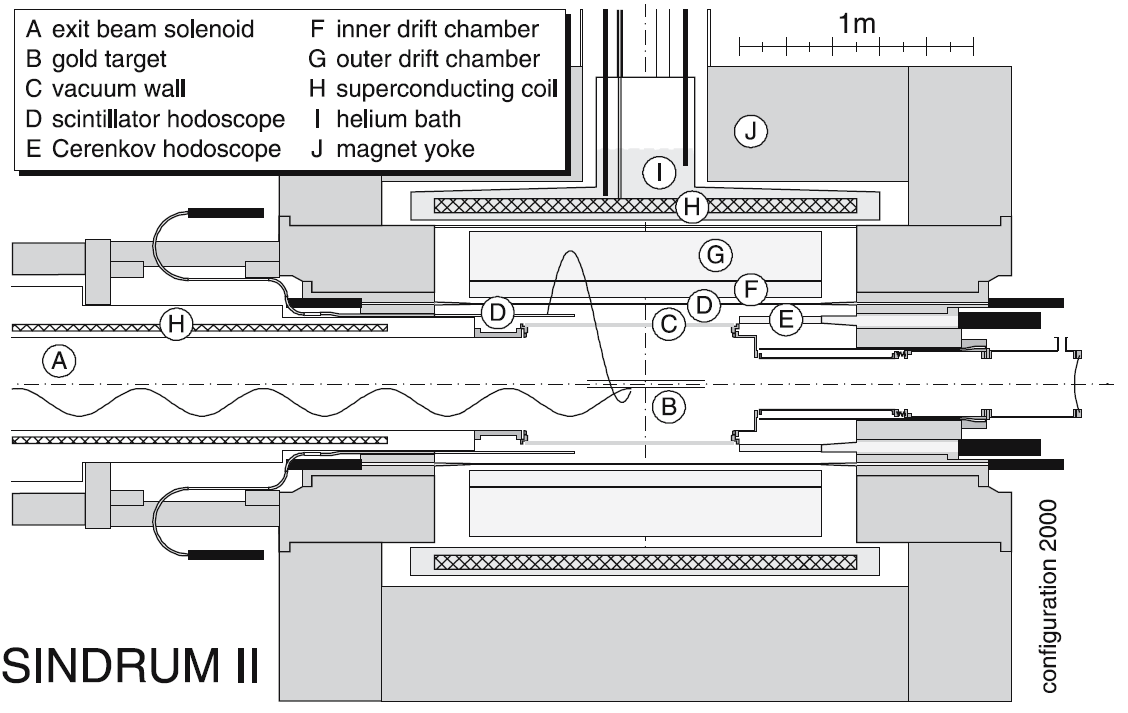
\includegraphics[scale=0.6]{SINDRUM_II}
\caption[SINDRUM II]{Pictorial view of the SINDRUM II experiment with the various section labeled as in the description \cite{SINDRUMII}.}
\label{_SINDRUM_II}
\end{figure}


\subsubsection{The Mu2e experiment at Fermilab}
Although Mu2e will be described extensively in the next Chapter, for comparison with COMET and DeeMee,
the key aspects of the experiment are also reported here.\\
Mu2e will use an 8 GeV, 25 kW pulsed proton beam, with 100 ns wide bunches separated by 1.7 $\mu$s.  
Fig. \ref{_MuonBeamline} shows a pictorial view of the experimental setup 
where the three sections of the experiment, respectively named
Production Solenoid, Transport Solenoid and Detector Solenoid, are visibile.  
The layout of the magnetic field around the production target is graded and allows to channel the produced particles in the section dedicated to the transport. 
In this second section, the gradient pushes the particles towards the stopping target, the S shape reduces the background 
due to neutral particles and performs a selection on the charge sign using eq. \ref{eq_D} and collimators: (almost) only negative muons of less than 100 MeV/c reach the stopping target. Downstream of the aluminum target the straw tube tracker and the crystal electromagnetic calorimeter are located. Both these detectors adopted a hollow-cylinder geometry: 
the tracker is made of crossed straw tubes grouped in 20 stations 
while the calorimeter is composed of two identical disks comprised by CsI crystals and read by SiPMs.
The expected Mu2e sensitivity with three years of data taking is $R_{\mu e}<3\times10^{-17}$ \cite{MTDR}.



\begin{figure}[h!]
\centering
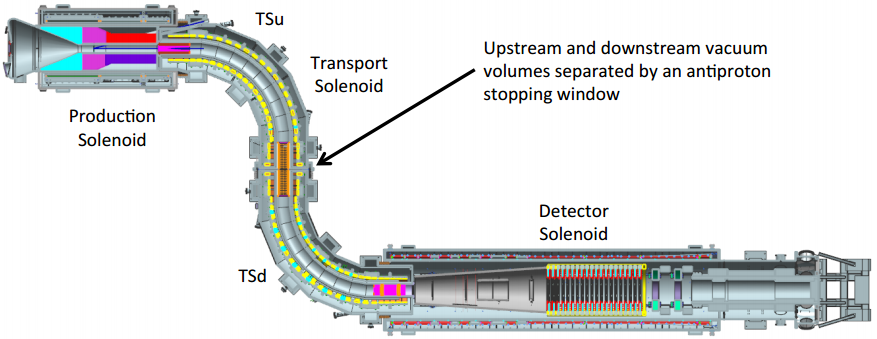
\includegraphics[scale=0.8]{MuonBeamline}
\caption[Mu2e experiment]{Pictorial view of the muon beam-line of the Mu2e experiment \cite{MTDR}.}
\label{_MuonBeamline}
\end{figure}

\noindent
Mu2e is being built by an international Collaboration which includes also the Italian Institute of Nuclear Physics,
responsible for the construction of the electromagnetic calorimeter.
The Mu2e Collaboration is also performing preliminary studies for the upgraded Mu2e II
\cite{Mu2e_II:2018}. 
The proton beam intensity will be increased by the PIP-II upgrade \cite{PIP_II:2018} 
that will increase the rate of stopped muons on target from $10^{10}\ \mu^-/$s (Mu2e) 
to $10^{11}\ \mu^-/$s. New detector technologies are under study for the upgraded Mu2e II.
The simulation shows that Mu2e II
sensitivity with three years of data taking will be $R_{\mu e} < \times10^{-18}$.

 


\subsubsection{The COMET experiment at J-PARC}
The COherent Muon-to-Electron Transition (COMET) experiment is being built at the Japanese Proton Accelerator Research Center (J-PARC) \cite{COMET_I}. 
Some of the key features are similar to Mu2e, 
like the beam used (a 8 GeV, 56 kW pulsed proton beam with a separation of $1.17\ \mu$s between the bunches). 
The two main differences between COMET and Mu2e are clear from the pictorial view reported in Fig. \ref{_COMET}:
\begin{itemize}
\item The presence of a C-shaped (not S-shaped) transport solenoid will allow a tighter muon momentum selection, 
traded with a reduced beam intensity $\sim 70\%$
\item An extra curved solenoid after the stopping target will remove most of the non interesting electrons 
before reaching the tracker.
\end{itemize}
COMET will be developed in two stages: Phase-I and Phase-II (Fig. \ref{_COMET}).
\paragraph{COMET Phase-I}
This first step will be useful to understand the experimental techniques and to study the backgrounds while setting an intermediate measurement at $R_{\mu e}\approx7\times10^{-15}$. 
The proton power will be limited to 3.2 kW and one simple 90$^\circ$ bend will be used. 
The major challenge is the short distance between the various elements and a cylindrical drift chamber will be used to track the electrons. For triggering and timing purposes, scintillating hodoscopes will surround the tracker. 
The TDR for COMET Phase I is \cite{COMET_I}.
\paragraph{COMET Phase-II}
The increased particle rate will be dealt with the introduction of a straw tube tracker 
and a crystal electromagnetic calorimeter exploiting LYSO crystals. 
The whole magnetic system will be expanded and refined.\\ \\
The driving forces behind the two-step approach are the uncertainties in the understanding of the physics processes. 
To begin with, the backward production by 8 GeV proton is poorly known, 
despite the results form the HARP experiment \cite{HARP}.
Then it must be underlined that the data on muon nuclear capture in aluminum are still quite scarce, 
although a joint effort of the Mu2e and the COMET collaborations led to the development of the AlCap experiment at PSI \cite{Edmonds:2015}\cite{AlCap:2015}\cite{AlCap:2018}. 
The goal of the AlCap collaboration has been to measure the rate and spectra of the particles ejected by muon capture in Aluminum to improve the physics models employed in the Monte Carlo simulations.

\begin{figure}[h!]
\centering
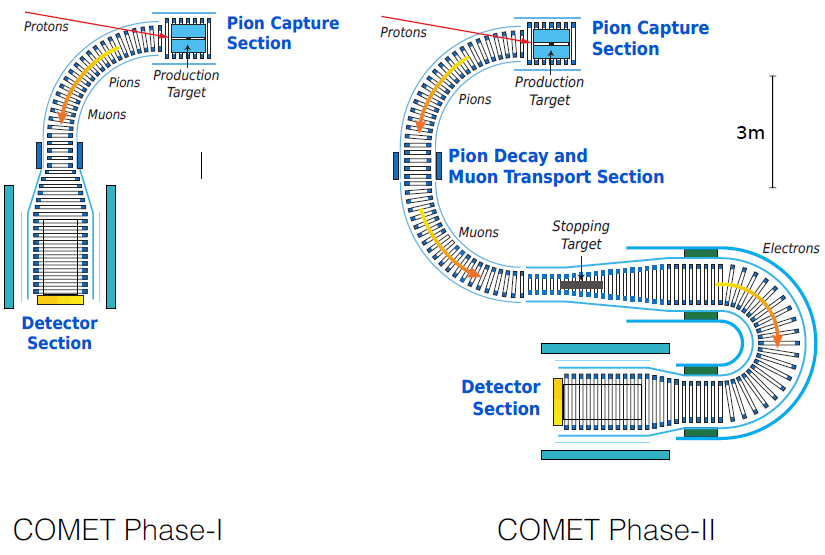
\includegraphics[scale=0.8]{COMET}
\caption[COMET experiment]{Pictorial view of the COMET apparatus \cite{COMET_I}.}
\label{_COMET}
\end{figure}

\subsubsection{The DeeMe Experiment at J-PARC}
The Direct emission of electron from Muon to electron conversion (DeeMe) \cite{DeeMe} experiment at J-PARC 
will use a simpler setup to search the muon-to-electron conversion. 
The experiment will be based on the new beam-line H-line, under development at the Muon Science Establishment, 
which will deliver 3 GeV protons (a pair of bunches, separated by 600 ns, at 25 Hz) on the production target. 
Some ($\mathcal{O}(10^{10})\ \mu/$s) muons will be stopped in the target itself and will allow 
to search for $\mu\rightarrow e$ using only one target. 
The experiment will use a high momentum beam line (H Line) 
which is currently under construction.\\
The signal will be reconstructed using multi-wire proportional chambers and a spectrometer. 
Low momentum background particles will be removed with a dipole in the transport system. 
The goal of the experiment is a single-event-sensitivty of $10^{-13}$ using a graphite target,
 and then of  $10^{-14}\div10^{-15}$ (depending on the running time) using a target of silicon carbide (SiC) 
 which has a higher capture rate. 
A pictorial view of the overall apparatus and time-structure of the events 
are shown in Fig. \ref{_DeeMe}.

\begin{figure}[h!]
\centering
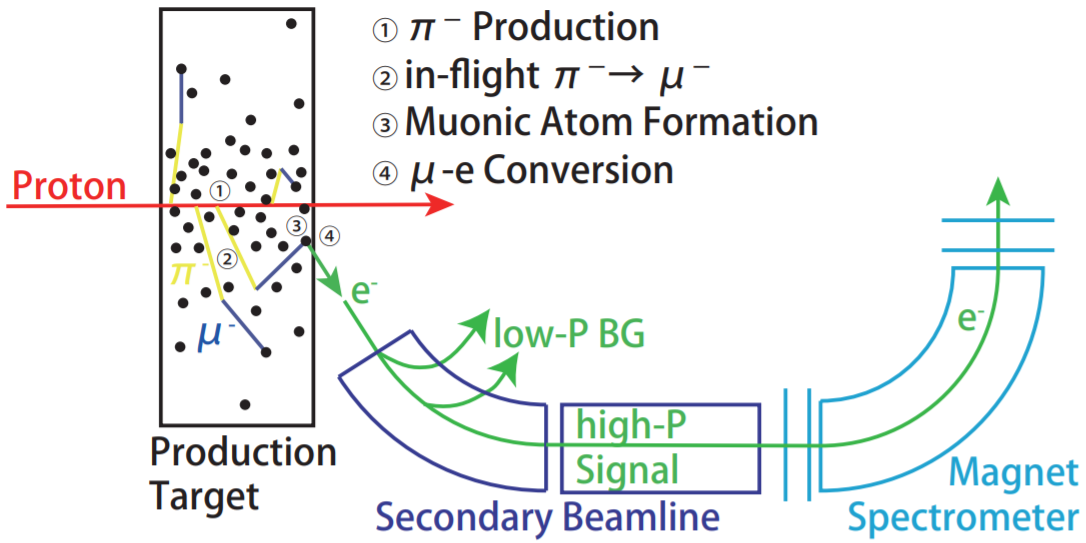
\includegraphics[scale=0.4]{DeeMe}
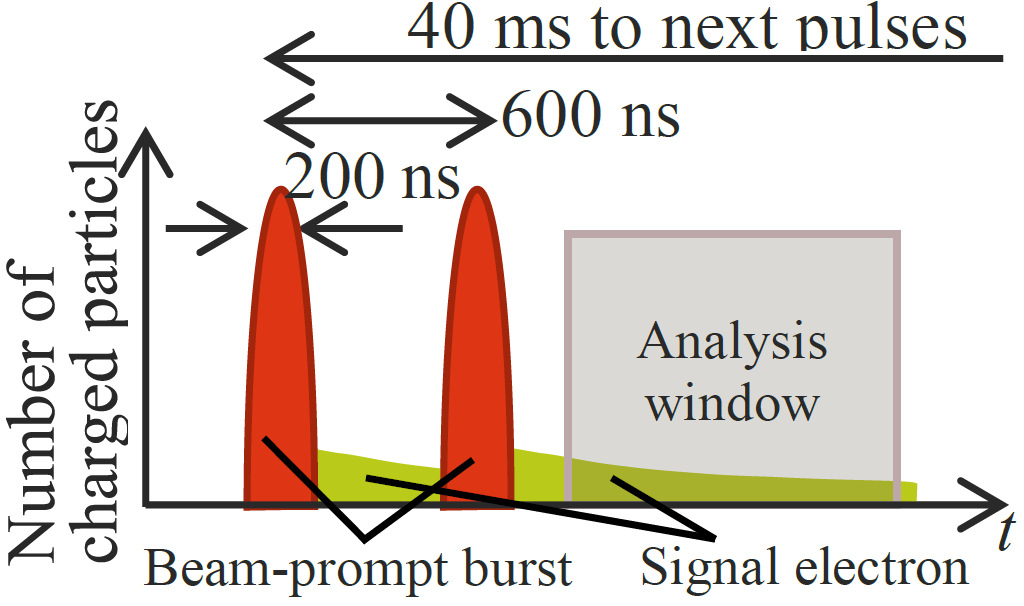
\includegraphics[scale=0.4]{DeeMe_event}
\caption[DeeMe experiment]{Pictorial view of the DeeMe apparatus and timing \cite{DeeMe}. }
\label{_DeeMe}
\end{figure}

%---------------------------
\chapter{The Mu2e experiment}
{\itshape 
Mu2e will search for the neutrino-less coherent conversion of a negative muon into an electron
in the field of an aluminum nucleus. The experiment will measure the ratio between the conversion 
and the nuclear muon capture rates:
\begin{center}
$R_{\mu e} = \frac{\mu^- + N(Z, A) \rightarrow e^- + N(Z, A)}
{\mu^- + N(Z,A) \rightarrow \nu_{\mu} + N(Z-1, A)}$
\end{center}
\noindent
The goal is to improve the current limit, set by the SINDRUM-II experiment \cite{SINDRUMII}, by four orders of magnitude and reach a SES (single-event-sensitivity) of $3\times 10^{-17}$ on the conversion rate, a 90\% CL of $8\times 10^{-17}$ and a $5\sigma$ discovery reach at $2\times 10^{-16}$.\\
Mu2e is currently under construction at the Fermilab Muon Campus by an international collaboration that includes the Italian National Institute of Nuclear Physics.
Data taking is planned to begin in 2023 and last for about three years. 
This Chapter provides a brief overview of the employed experimental techniques and infrastructures. Fundamental bibliography for this chapter was: \cite{signorelli} \cite{bob_cflv} \cite{bob_mu2e} \cite{Manolis}}

check where to put \cite{Measday:2001}

%\noindent
%(Spostare la Figura 2.1: An overview of the apparatus was already shown in fig. \ref{_mu2e_apparatus_pre} and in fig. %\ref{_MuonBeamline} shows a preview of the magnetic system that will be described shortly. })


%\begin{figure}[h!]
%\centering
%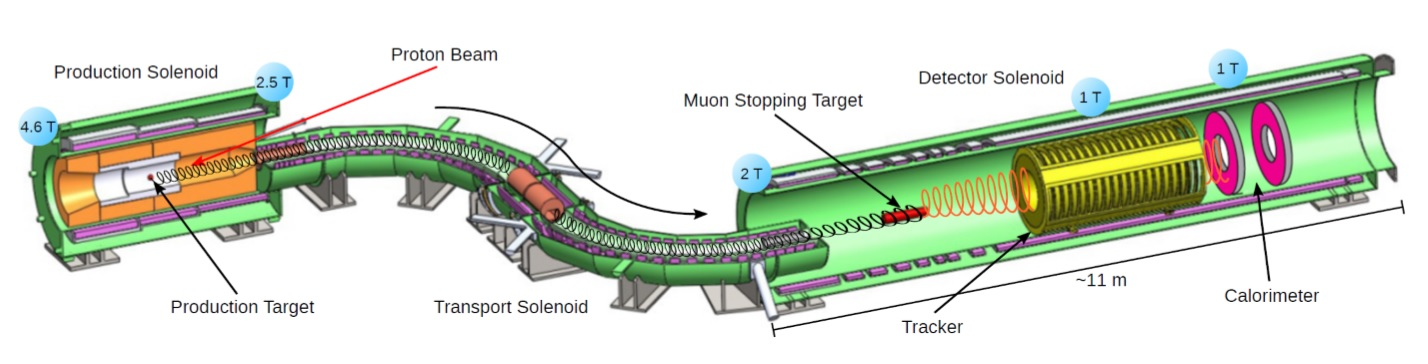
\includegraphics[scale=0.6]{mu2e_apparatus}
%\caption{Spostare: mu2e apparatus}
%\label{_mu2e_apparatus_pre}
%\end{figure}

\section{Signal and backgrounds}

The experimental signature of the $\mu N \rightarrow eN$ process is one mono-energetic  \textit{conversion electron} (\textit{CE}), with energy close to the muon rest energy, that recoils off the nucleus in a two-body interaction.
The energy of the electron is $E_{CE} = m_\mu -B(Z) -E_R(A) \approx 104.97$ MeV, where  $B(Z)\approx\frac{Z^2\alpha^2m_\mu}{2}$ is the muonic binding energy  and $E_R\approx\frac{m_\mu^2}{2m_N}$ is the recoil energy of the nucleus.
Although very few background processes in Mu2e can generate an electron of this energy, the single event sensitivity the experiment wants to achieve requires that these processes are understood in great detail. 
This is a challenging task and the Mu2e Collaboration is dedicating a great effort to the development of the simulation of the experimental apparatus and to the study of the sensitivity. 
Fig. \ref{_signal_bg} shows the reconstructed momentum spectrum of selected tracks from muon decay-in-orbit (DIO) and other backgrounds reconstructed with the full Mu2e simulation. 
The expected signal from conversion electrons assuming $R_{\mu e} = 2 \times 10^{-16}$ is overlaid. 

\begin{figure}[h!]
\centering
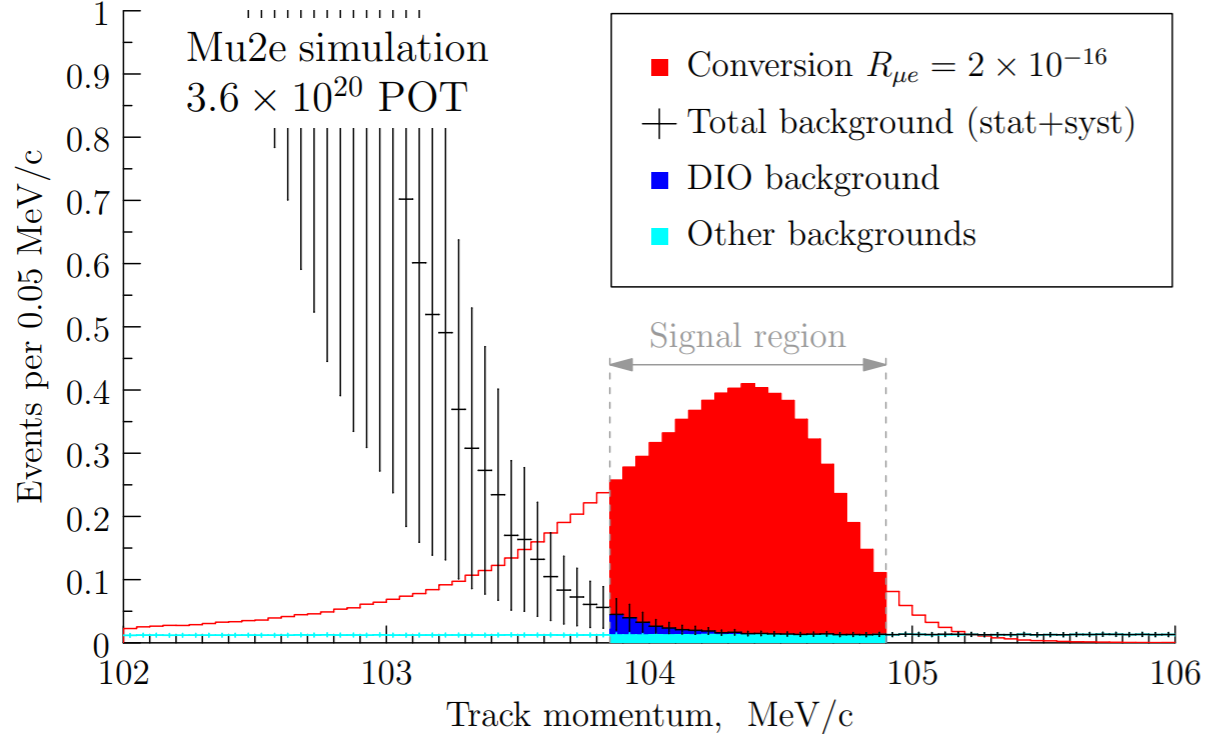
\includegraphics[scale=0.6]{signal_bg}
\caption[Mu2e simulated signal]{Simulated momentum spectrum for muon decay-in-orbit (DIO) events and conversion electron (CE) events estimated assuming $R_{\mu e} = 2 \times 10 ^{-16}$. 
The distributions are normalized to the total number of muons expected for $3.6 \times 10^{20}$ protons on target. 
The signal window is limited to the range $103.9 < p < 104.9$ MeV/c \cite{Manolis} \cite{CD3}.}
\label{_signal_bg}
\end{figure}

\noindent Conceptually, the main background sources can be grouped in three categories: 

\begin{itemize}
\item Cosmic rays: cosmic muons traversing the detector region can decay into electrons, be misidentified as electrons, or generate electrons in the interaction with the stopping target, that can be misidentified for signal conversion electrons; 
\item Intrinsic backgrounds: this source of background is generated by the same muons used to perform the conversion signal search and the measurement of $R_{\mu e}$. 
It consequently scales with the stopped muon flux and the number of protons on target. 
The largest contribution is due to the decay in orbit (DIO) of muons captured by the Aluminum nuclei. 
The need to minimize this background source has played a primary role in determining the resolution that the Mu2e detector system requires.
\item Beam-related backgrounds: these sources of background are associated to the generation and transport of the muon beam. 
The main contribution is due to radiative pion captures (RPC) and it is the primary reason for using a pulsed proton beam with a timing structure specifically optimized  for Mu2e. 
\end{itemize}
In the following we will provide a more detailed description of the background sources mentioned above.
Table \ref{T_backgrounds} reports the summary of the expected number of events for each source as reported in \cite{CD3} corresponding to $3.6 \times 10^{20}$ ``live-time'' protons on target; along with the current preliminary results obtained in the effort of updating the sensitivity estimate. 
Under the \textit{other} category are the small contributions like the decay in flight of both muons and pions ($<0.003$ and $\sim 0.001$ background events) as well as muonic radiative capture and electrons from the beam.

\begin{comment}
\begin{figure}[h!]
\centering
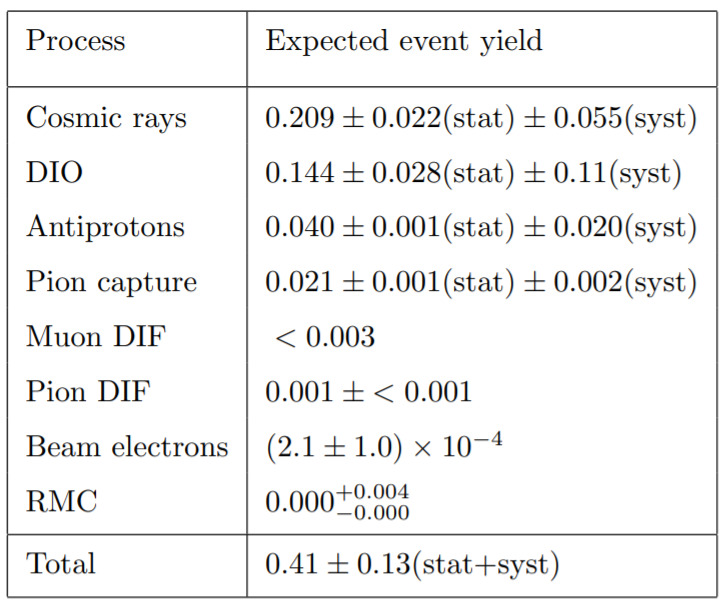
\includegraphics[scale=0.7]{CD3_backgrounds}
\caption[Mu2e background]{CD3 backgrounds}
\end{figure}
\end{comment}

\begin{table}
\centering
\begin{tabular}{|c|c|c|}
\hline
Process & Yield (CD3) & Yield (preliminary)\\
\hline
\hline
CR	&	$0.209(22)_{stat}(55)_{syst}$ & $0.18\pm0.05$ \cite{CRV_now}\\
\hline
DIO	&	$0.144(28)_{stat}(110)_{syst}$ & \\
\hline
$\overline{p}$	&	$0.040(1)_{stat}(20)_{syst}$ &$0.04 \div 0.4$ \cite{Giovanni:2020}\\
\hline
RPC	&	$0.021(1)_{stat}(2)_{syst}$	& 0.025 \cite{RPC_now} \\
\hline
\textit{other}	& $< 0.004$ &\\
\hline
\hline
Total &	$0.41(13)_{stat+syst}$ &\\
\hline
\end{tabular}
\caption[Mu2e background]{Blessed estimates in CD3 \cite{CD3} of the backgrounds for the Mu2e experiment.
The chosen momentum window for the signal search is $[103.85, 104.90]$ MeV$/c$ and the beam extinction is assumed $10^{-10}$. 
The corresponding sensitivity is $SES=(3.01 \pm 0.03(stat) \pm 0.41(syst)) \times 10^{-17}$. 
The update of the sensitivity is an ongoing effort and the new estimate is expected this year.}
\label{T_backgrounds}
\end{table}

\subsection{Cosmic rays (CR)}
The background generated by cosmic rays is a problem encountered in many experiments.
The simulation shows that this is the main source of background in Mu2e (Table \ref{T_backgrounds})
and this is due to two contributions:

\begin{itemize}
\item Cosmic muons can interact with the detectors material and be erroneously reconstructed as electrons, or they can simply decay into electrons as they pass through the volume in which the detectors are located. 
This source of background can be reduced to a negligible level by properly exploiting the combined tracker and calorimeter data.
\item A cosmic muon could knock out of the stopping target an electron with energy close to conversion electron energy ($E_{CE}$). 
That electron would be completely indistinguishable from a conversion electron. 
Similarly, an electron could also be knocked out from some material located upstream of the stopping target and be captured by the magnetic field. 
This source of background could reach the level of one event in the signal region per day.
For this reason the Mu2e Collaboration has decided to develop and build the Cosmic Ray Veto system.
\end{itemize}
The determination of the yield of this background source is an ongoing effort but the current preliminary estimate is $0.18\pm0.05(stat)$ \cite{CRV_now}.

\subsection{Muon decay in orbit (DIO)}
There is a significant difference between the electron energy spectrum of a free-muon decay and a decay in orbit, and this difference is the source of the muon decay in orbit (DIO) background.
In the hypothesis of negligible neutrino masses, the Michel spectrum has an end point at $E_{max}=\frac{m_\mu^2+m_e^2}{2m_e^2}\approx52.8$ MeV, which is way below the energy of 105 MeV expected for a conversion electron.
On the other hand, for a bound muon decay, the electron can exchange a photon with the nucleus and this effect modifies the electron energy spectrum. 
Sergent's rule provides the spectrum behaviour near the end point that is of the order of $(E_{CE}-E_{DIO})^5$, while Czarnecki and others have calculated the spectrum including radiative corrections \cite{Czarnecki} \cite{Czarnecki2015}.
The resulting spectrum is shown in fig. \ref{_DIO}.
A quick analysis of the right-hand side of the spectrum provides a back-of-the-envelope estimate of the necessary resolution: a measurement at $\mathcal{O}(10^{-17})$ would require at least $10^{17}$ muons. 
The Czarnecki spectrum shows we could expect $\sim1$ event within 1 MeV from the conversion electron energy. 
As a rough estimate, the momentum resolution must therefore be $\approx1$ MeV$/c$. 
The detailed Mu2e simulation yields $<180$ keV$/c$, which in the following is assumed as requirement.\\

\begin{figure}[h!]
\centering
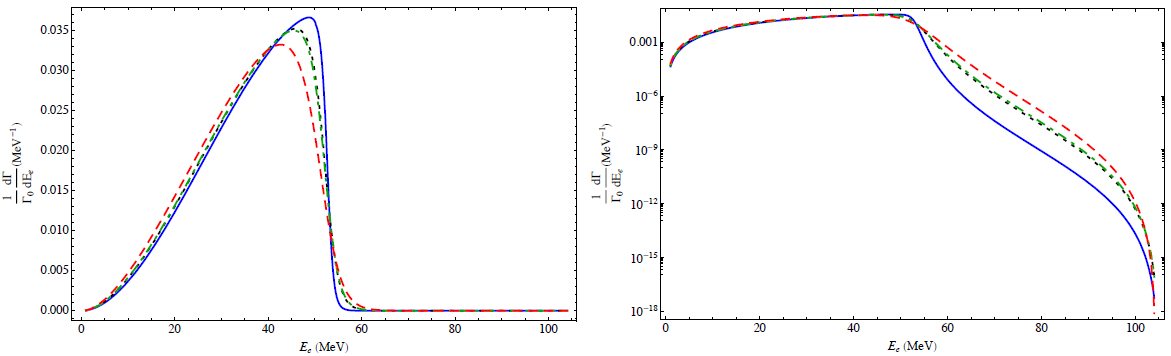
\includegraphics[scale=0.8]{DIO_materials}
\caption[Decay In Orbit spectra]{Electron spectrum as determined from different materials
and normalized to the free-muon decay rate \cite{signorelli}. 
The solid blue line is for carbon, the black dotted line for aluminum, 
the green dot-dashed line for silicon and the red dashed line for titanium.}
\label{_DIO}
\end{figure}

\subsection{Radiative Pion Capture (RPC)}
One of the main beam-related sources of background is due to the process
$\pi^- N \rightarrow \gamma N^\prime$ where $N^\prime$ is an excited nuclear state. 
Since the photon spectrum peaks around 110-120 MeV, this process can generate
a background if there is an asymmetric photon conversion that produces
an electron with the energy in the range of the conversion electron energy. 
This conversion can happen both \textit{internally} ($\pi^- N \rightarrow e^+e^- N^\prime$) or \textit{externally}
in the material of the stopping target.
By numerical coincidence, the internal and external conversion probabilities for the Mu2e target and geometry are approximately equal. 
At the same time, the number of $e^-$ generated by external conversion is larger than the number of $e^+$, 
since Compton scattering can knock out only $e^-$.\\
The existence of the RPC background is the main reason for the timing structure of the Mu2e \textit{event} (Fig. \ref{_mu2e_event}). 
In Mu2e 'jargon' an \textit{event}  is the time period between two consecutive proton pulses on the production target. 
Although there are  uncertainties on the timing of the proton beam, 
the duration of an event is approximately $1.7\ \mu$s. 
After the proton pulse, some time is required to collect and propagate pions and muons generated in the collision 
and the timing of the data acquisition gate is chosen to maximize the signal to background ratio.
The RPC background is minimized by delaying the active window
with respect to the pion arrival time. 
The Mu2e simulation shows that the number of pions can be suppressed 
by a factor $\mathcal{O}(10^{11})$ 
if the measurement period begins at about 700 ns from the proton pulse.
This estimate derives from a combination of the beamline transit time 
and pion lifetime.
In practice, Mu2e will wait for the number of pions contaminating the beam 
to have been sufficiently reduced to reach a manageable level of background.
The Data acquisition gate is approximately 200 ns wider than the actual Selection window
to increase the amount of available data to study the backgrounds.
This technique is effective as long as the ratio between out-of-time protons 
(i.e. protons outside the pulse) and in-time protons (i.e. protons inside the pulse)
is kept below $10^{-10}$. 
An \textit{extinction} system and monitor are thus necessary to keep this effect
under control.
The current estimate of the overall yield for radiative pion captures is under study 
and a preliminary result is $\approx 0.025$ \cite{RPC_now}.

\subsection{Antiprotons}
\label{sec:antiprotons}
The background due to  antiprotons is quite complex. 
These particles are generated in the production target and are collected, like muons and pions, toward the stopping target. 
Antiprotons have lower momentum than most particles collected by the muon beam-line and most of them stop and annihilate in the stopping target, thus generating $\pi^0$. 
Pions are a source of photons which can convert asymmetrically in an energetic electron.
The non-trivial component to account for rise when accounting for antiprotons interacting in the muon beamline and the various possible outcomes.\\
There are a number of elements introduced in the muon beam-line to reduce the yield of stopped $\overline{p}$ in the stopping target but, in order to not reduce the muon yield, these elements cannot be too aggressive. 
On top of that, the production mechanisms of $\overline{p}$ in $pp$ collision is still poorly known, particularly in the backward direction and multiple models are being compared.
A lot of effort is undergoing to improve the level of  understanding of this contribution and the models behind the simulations. 
The current estimate is $0.04 \div 0.4$ \cite{Giovanni:2020} but it is limited by the understanding of some specific processes simulation model in Geant4 which are under study.

\begin{figure}[!htb]
\centering
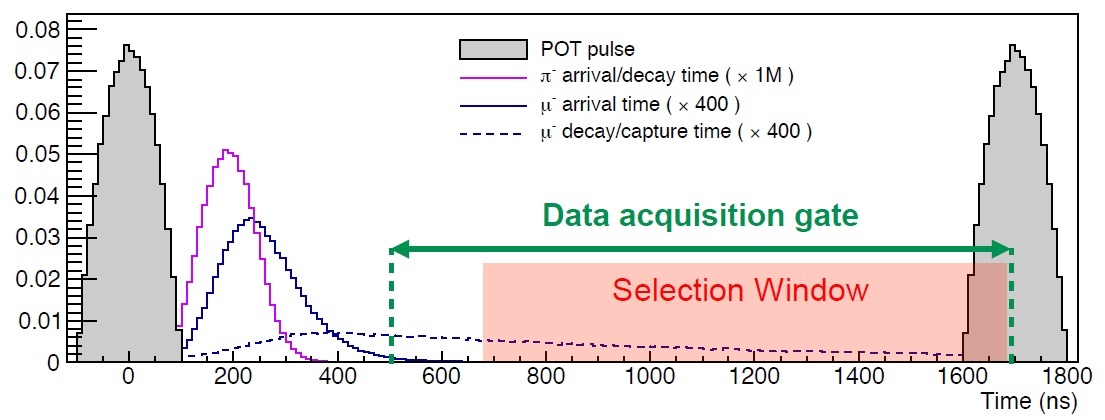
\includegraphics[scale=0.7]{mu2e_event}
\caption[Mu2e event timing]{The Mu2e beam timing \cite{bob_mu2e}: the proton pulse arrives every 1.7 $\mu$s (shaded); 
$\pi$ and $\mu$ arrival time at the detector solenoid (purple and blue);
$\mu$ decay and capture time (dashed).
The Selection window ([700,1700] ns) is the period of time for which Mu2e will analyze data but the data acquisition gate will be roughly 200 ns larger.}
\label{_mu2e_event}
\end{figure}

\subsection{Protons}
\label{backgrounds}
Although protons generated in the stopping target constitute a negligible source of background for the conversion electron search, they represent one of the main causes of occupancy in the tracker. About $61\%$ of stopped muons undergo \textit{nuclear capture} though the process $\mu^-(Z,A)\rightarrow \nu_\mu X$. 
Understanding $X$ is beyond the scope of this Thesis and is still the subject of intense studies within the Mu2e Collaboration, but we know it is a final state consisting of the residuals of the nucleus and a number of possible ejected particles. 
Among the various possibilities, ejected protons and deuterons are extremely important since they are highly ionizing and can compromise detectors performance. 
The characterization of the spectra of these particles will be discussed in Chapter 4, when will be discussed how their reconstruction can be a useful tool as a monitoring system of the experiment.


\section{The accelerator complex}
\label{sec:beam}
The Fermilab accelerator complex is the infrastructure which provides 
the proton beam with kinetic energy of 8 GeV necessary to generate 
the high intensity muon beam employed by the Mu2e experiment.
The accelerator complex 
(Fig. \ref{_ProtonBeamlineArial} and \ref{_ProtonBeamlineArial_sketch})
is schematically composed of the following stages:
\begin{itemize}
\item A Cockcroft-Walton generator turns hydrogen gas
into H$^-$ ions owing it into a container lined with molybdenum electrodes. 
A magnetron then generates a plasma to form H$^-$ ions close to the metal surface. 
The electrostatic field generated by the Cockcroft-Walton accelerates the ions out of the container;
\item A Linac accelerates the H$^-$ ion beam up to the energy of approximately 400 MeV. 
Then the H$^-$  ion beam goes through a carbon foil, 
where electrons are lost, and produces a proton beam;
\item The Booster Ring accelerates the proton beam to the kinetic energy of approximately 8 GeV;
\item The Recycler Ring re-bunches the protons. 
The resulting beam, with reformatted bunches of $4\times10^{12}$ protons 
and kinetic energy of 8 GeV,
is synchronously transferred to the Delivery Ring;
\item Through resonant extraction from the Delivery Ring proton micro-bunches
with $3.9\times10^7$ particles are injected into the Mu2e beam-line every $1.7 \mu$s. 
This  micro-bunch structure determines the Mu2e beam timing shown in Fig.  \ref{_mu2e_event}. 
\end{itemize}

\begin{figure}[h!]
\centering
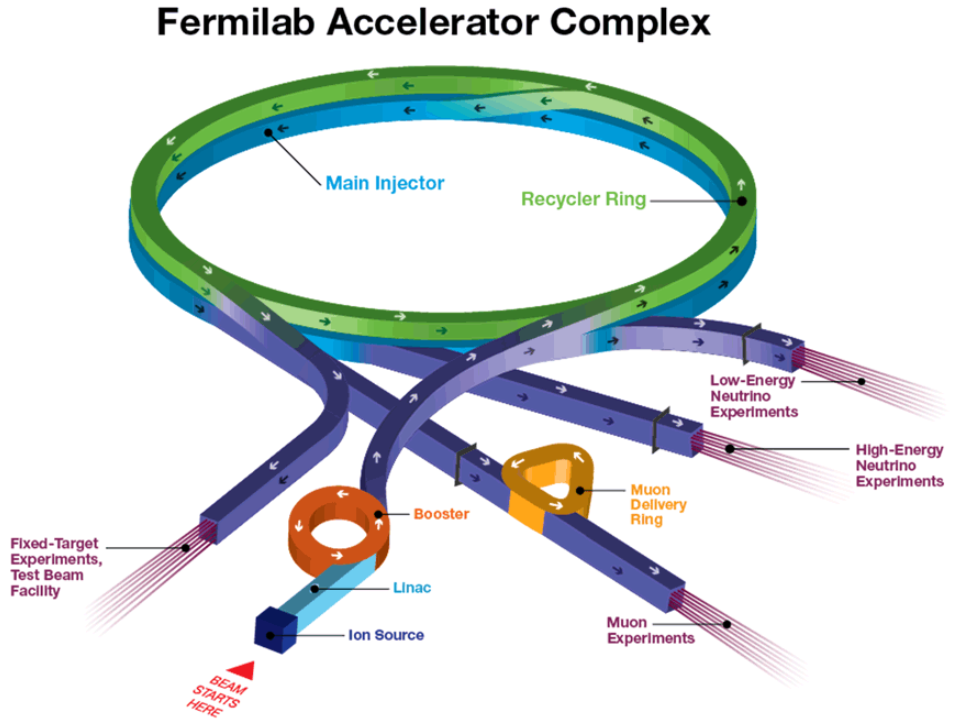
\includegraphics[scale=0.5]{ProtonBeamlineArial_3D}
\caption[Fermilab accelerator complex]{Pictorial view of the Fermilab accelerator complex that provides the proton beam to the Mu2e experiment \cite{FNAL}. 
Protons are transported from the Booster to the Recycler Ring where they circulate while being re-bunched. 
The reformatted bunches are transported to the Delivery Ring where they are slow-extracted to the Mu2e detector through a new external beam-line.}
\label{_ProtonBeamlineArial}
\end{figure}

\begin{figure}[h!]
\centering
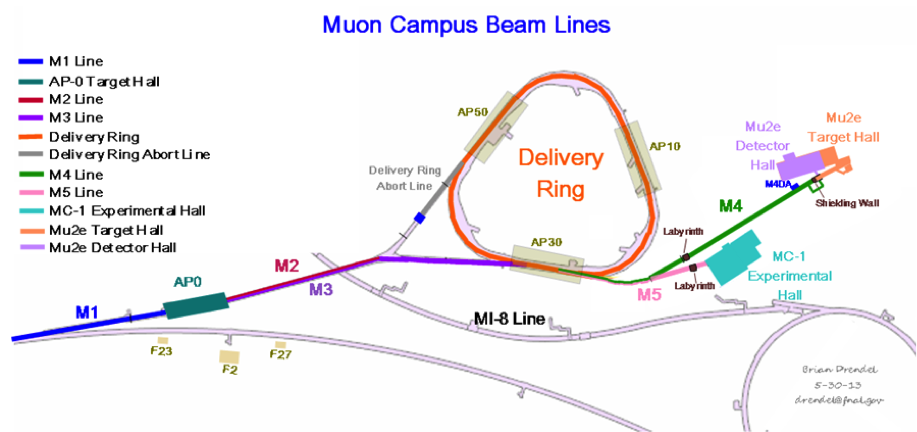
\includegraphics[scale=0.7]{ProtonBeamlineArial_sketch}
\caption[Mu2e delivery system]{A schematic more specific of the Mu2e facility and accelerator complex \cite{MTDR}. 
The beam-lines are described in \cite{MTDR}.}
\label{_ProtonBeamlineArial_sketch}
\end{figure}

\begin{figure}[h!]
\centering
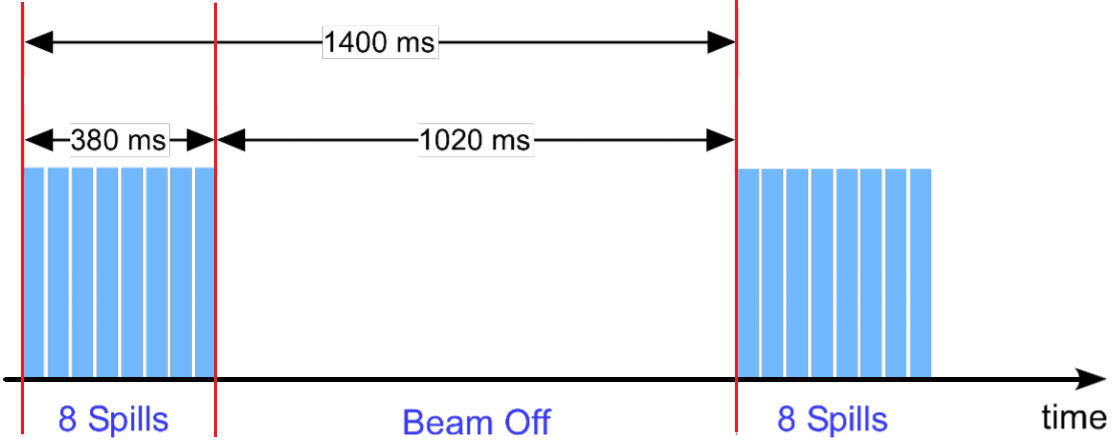
\includegraphics[scale=0.6]{beam_time_structure_2}
\caption[Mu2e proton beam time structure]{Time structure of the proton beam produced by the Delivery system \cite{BeamStruct}. 
Supercycles are split between the Mu2e and NO$\nu$A experiments. 
The ON period for Mu2e is approximately 380 ms and is divided in eight spills. 
The duration of a spill is 43.1 ms and each spill is composed of a train of micro-bunches 
separated by $1.7 \mu$s.}
\label{_beam_time_structure}
\end{figure}

\noindent
The resulting time structure of the train of proton pulses is shown in Fig. \ref{_beam_time_structure}.
The \textit{supercycle} takes 1.4 s and is divided in the ON-beam (379.8 ms) and OFF-beam (1020.2 ms) sections. 
Only the ON-beam section is delivered to Mu2e, the OFF-beam section is reserved for NO$\nu$A.
The ON-beam section is further subdivided in eight 43.1 ms trains of micro-bunches
named \textit{spills} and  separated by 5 ms gaps.\\
The micro-bunches are created by resonant extraction \cite{Extraction}: 
first the beam is pushed to an unstable motion to keep it not centered (achieved by changing the phase-space distribution of the beam through the usage of sextupoles); 
then the system illustrated in fig. \ref{_Extraction} separates a fraction of the bunch  
and sends it towards the Mu2e experiment. 
The fraction of the beam outside the stable orbit enters in the ElectroStatic-Septum and is kicked. 
To reach the necessary separation the procedure is done twice and quadrupole are inserted to keep the rest of the bunch from diverging.
The last element has two channels: one is field free and is used by the bunch while the other kicks the $\mu$-bunch outside the Delivery ring.

\begin{figure}[h!]
\centering
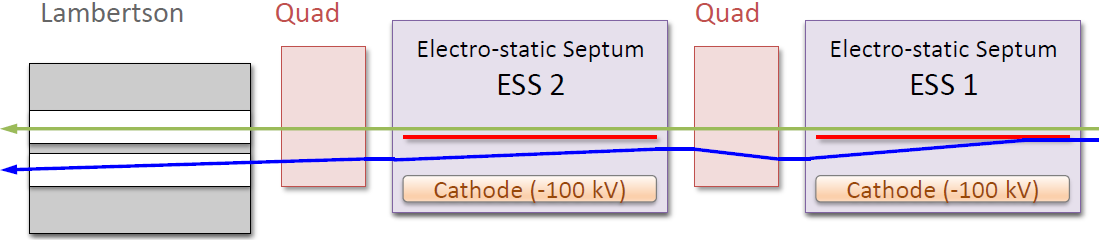
\includegraphics[scale=0.7]{Extraction}
\caption[Resonant extraction]{The extraction method, with the beam moving from right to left \cite{Extraction}. A foil plane (red line) in the septa allows to kick horizontally only the beam on one side. The two quadrupoles are used for horizontal and vertical focusing. The last magnet has a field free channel while the other kicks the beam outside the Delivery Ring.}
\label{_Extraction}
\end{figure}

\noindent 
One of the most important parameters that characterizes the proton beam quality is the 
\textit{extinction factor} that measures the fraction of protons on the
target between to consecutive beam pulses. The extinction factor should be 
as low as possible, since \textit{out of time} protons can generate the background due to Radiative Pion Captures. 
Mu2e has set the upper threshold on the extinction factor $10^{-10}$. 
This value will be achieved by employing a high frequency AC dipole and a complementary monitor system. The effect of the AC dipole is shown in fig. \ref{_AC_dipole} and \ref{_Extinction}.\\

\begin{figure}[h!]
\centering
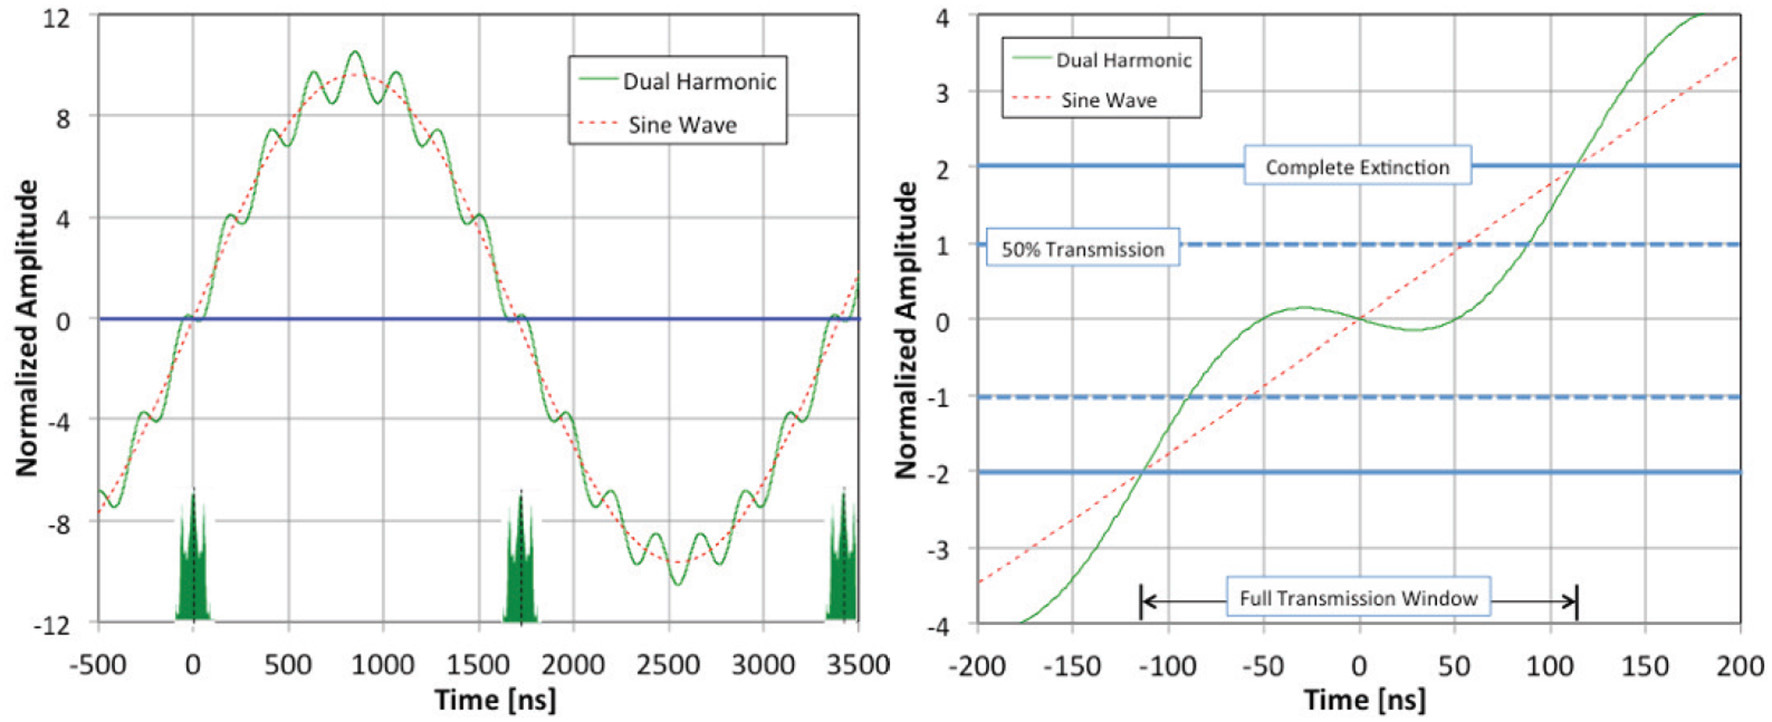
\includegraphics[scale=0.5]{AC_dipole}
\caption[AC dipole extinction]{The AC dipole system sweeps out-of-time beam into the collimators \cite{bob_mu2e}. 
The left-hand plot shows the normalized amplitude of the field and inset is also shown
the location in time and the expected shape of the proton pulses. 
The right-hand plot shows the normalized amplitude of the displacement: 
if the value is 1 the center of the beam is deflected to the edge of the collimators (50\% transmission); 
if the value is 2 the entire beam is deflected into the collimators.}
\label{_AC_dipole}
\end{figure}

\begin{figure}[h!]
\centering
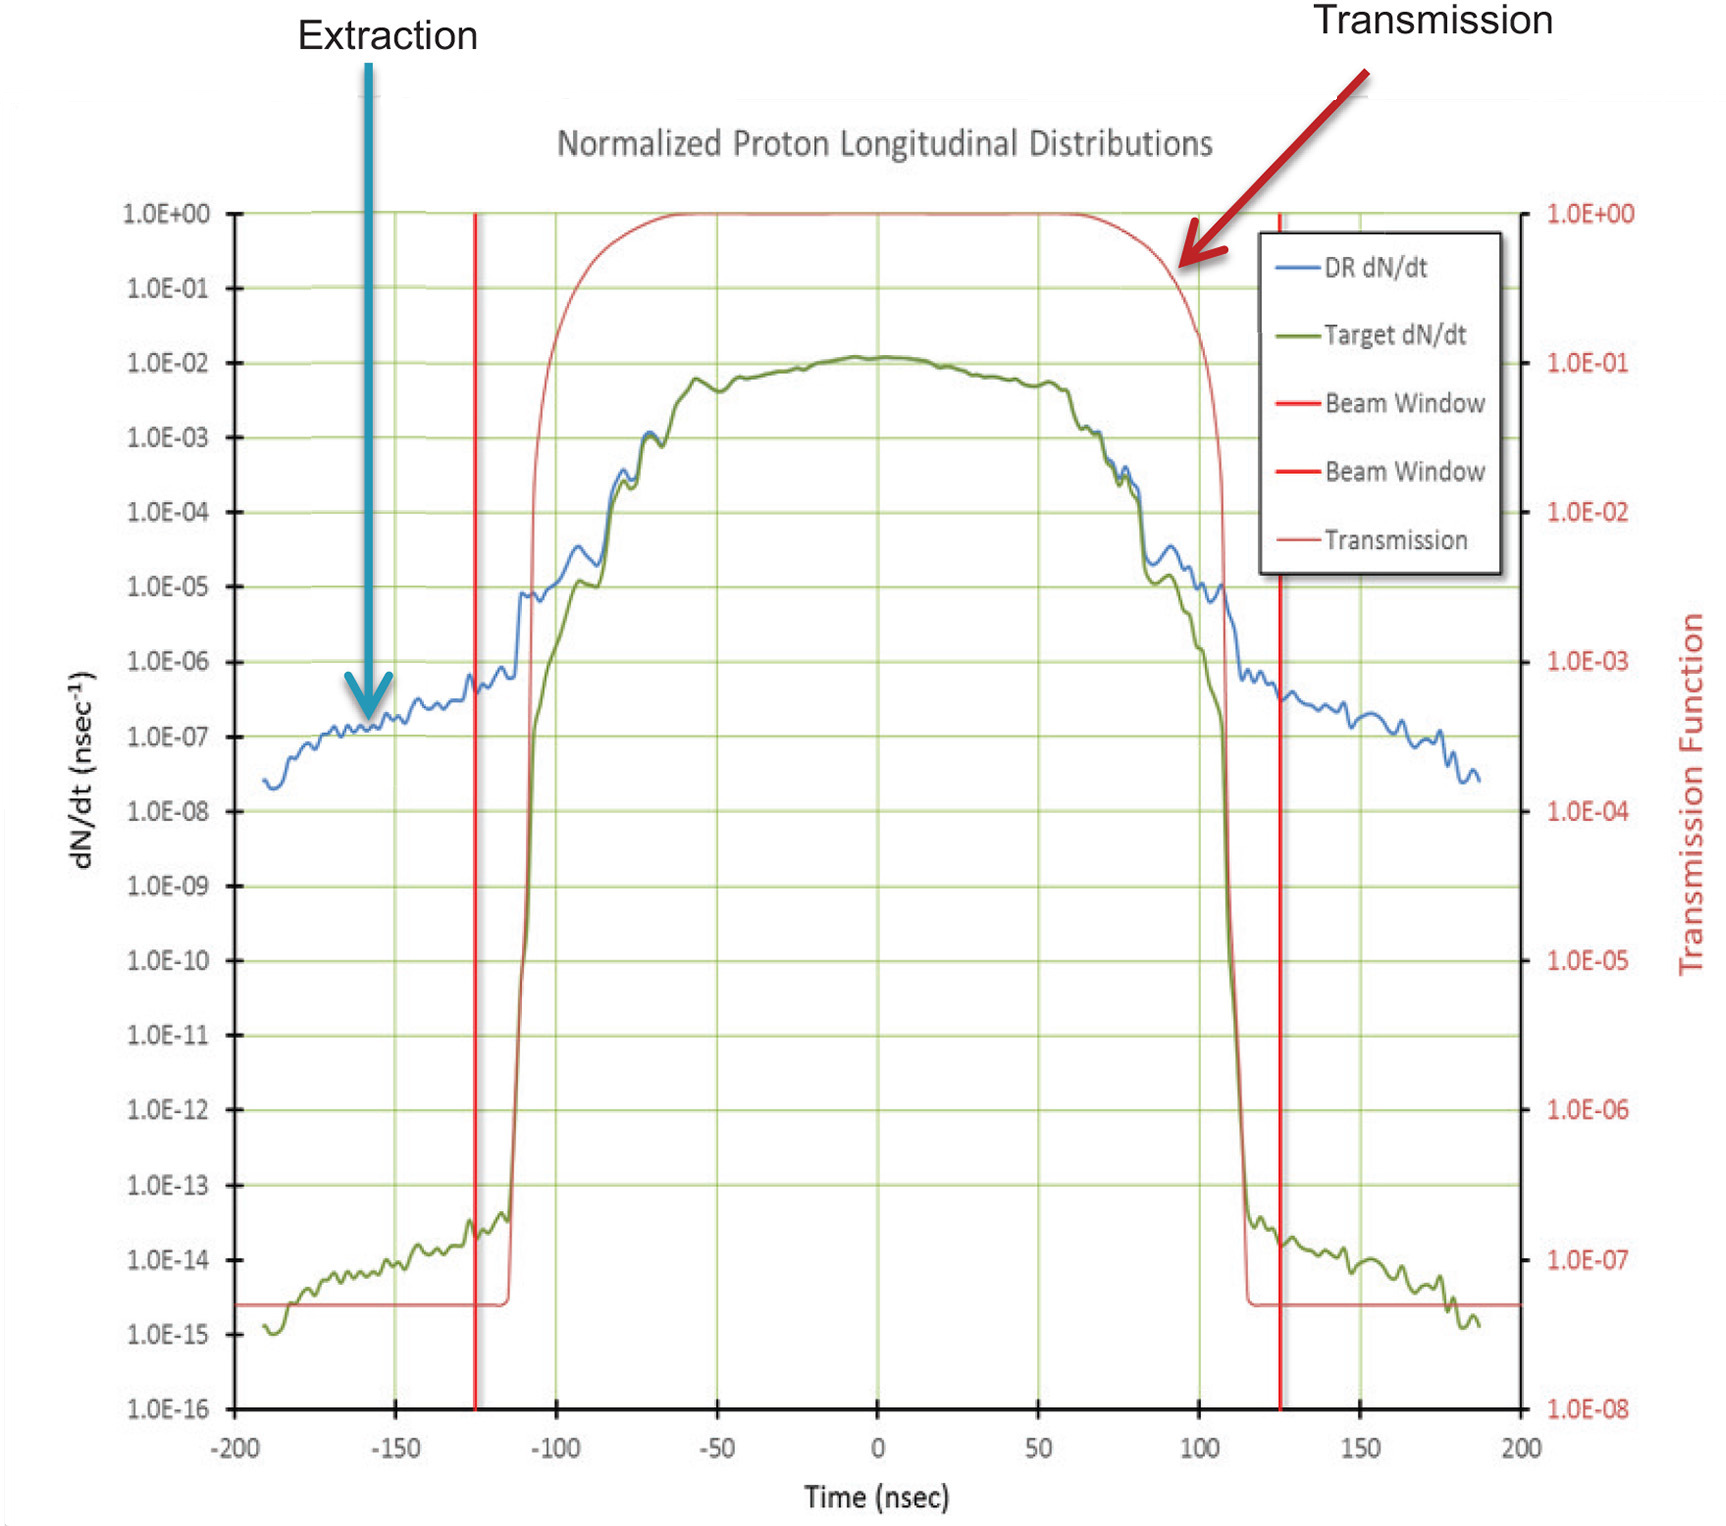
\includegraphics[scale=0.3]{Extinction}
\caption[AC dipole extinction performance]{Performance of the AC dipole system\cite{bob_mu2e}. The red line (scale at left) shows the transmission curve of the external dipole/collimator system (G4Beamline simulation \cite{G4beamline}). The green curve (scale at right) shows the beam extracted from the Delivery ring (ESME simulation \cite{ESME}). The blue curve shows the convolution of the two.}
\label{_Extinction}
\end{figure}

\subsection{Protons On Target}
The proton bunches will have an approximate transverse radius of about 1 mm, a duration of about 250 ns and an arrival time deviation of less than 10 ns.
The resonant extraction typically creates non-uniform pulses with a long tail of high intensity pulses. 
The Spill Duty Factor measures the relative spread of the pulse intensity distribution and has been used to set the requirement \cite{BeamRequirements}:
$$SDF=\left(1+\left(\frac{rms}{I}\right)^2\right)^{-1}$$
The value of {\em SDF} equal to 100\% (pulse intensity {\em rms} = 0) corresponds to a completely uniform spill. 
If the pulse intensity {\em rms} increases, {\em SDF} decreases and the spill becomes less uniform.
The spill quality requirement for Mu2e is to have {\em SDF} $\geqslant$  60\%.
The extraction is still under study but the fluctuations for the intensity are expected to be on a timescale of ms: 
this estimate is one of the driving forces behind the work described in this Thesis and will be discussed 
in Chapter 4 in more detail.\\
The Mu2e Collaboration has performed numerous simulations of the beam structure and, 
although still preliminary, the simulation described in \cite{SpillSim} will be employed in this Thesis. 
The distribution of the intensity of the bunches is shown in fig \ref{_POT_distribution} 
while the time dependence of the fraction of the pulse intensity during a spill is shown in fig. \ref{_POT_sim}. 
It is important to notice that the interesting structures in the time dependence 
visible in Fig. \ref{_POT_sim} are on the time scale of ms.
\label{_Fluctuations}

\begin{figure}[h!]
\centering
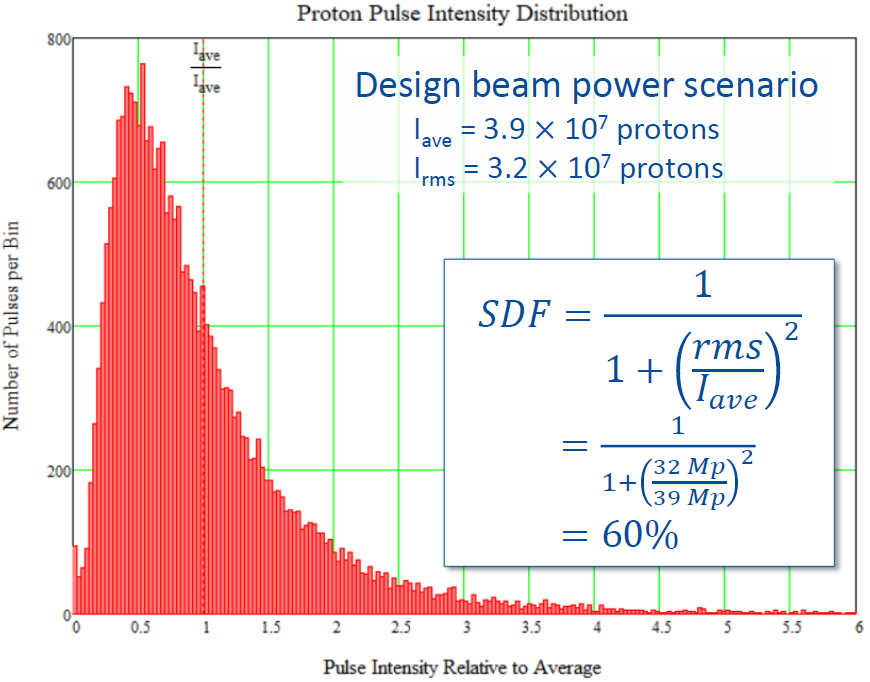
\includegraphics[scale=0.7]{POT_distribution}
\caption[Proton pulse intensity]{Simulated proton pulse intensity distribution \cite{SpillSim}: 
number of pulses on the vertical axes and relative intensity of a micro-bunch on the horizontal. 
This distribution is updated every time a section of the accelerating and delivery system is tested.}
\label{_POT_distribution}
\end{figure}

\begin{figure}[h!]
\centering
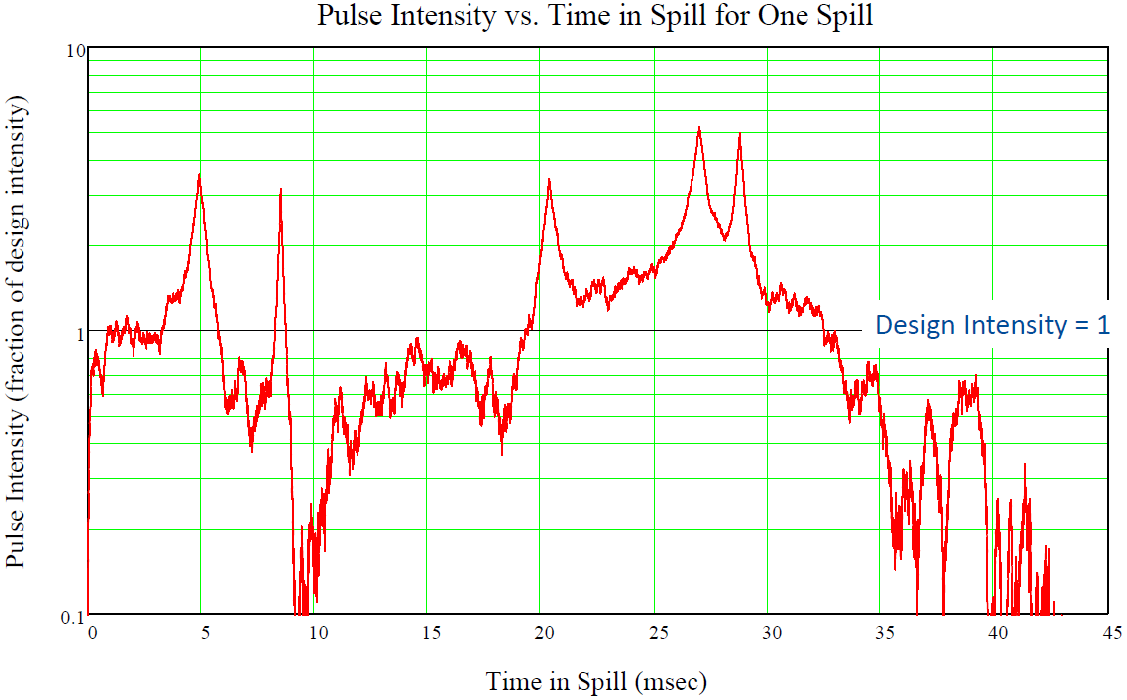
\includegraphics[scale=0.6]{POT_sim}
\caption[Proton pulse intensity fluctuations]{Simulation of the pulse intensity computed as a fraction  
of the design intensity and 
as function of time in a spill for one spill \cite{SpillSim}.}
\label{_POT_sim}
\end{figure}

\section{The Mu2e magnetic system}
The basic principle of the Mu2e experiment is to use a sophisticated magnetic system (Fig. \ref{_mu2e_apparatus_pre}) 
to form the high-intensity muon beam by collecting and filtering the particles emerging from the stopping target. 
The magnetic system is probably the most innovative, challenging and essential part of the entire experiment. 

\begin{figure}[h!]
\centering
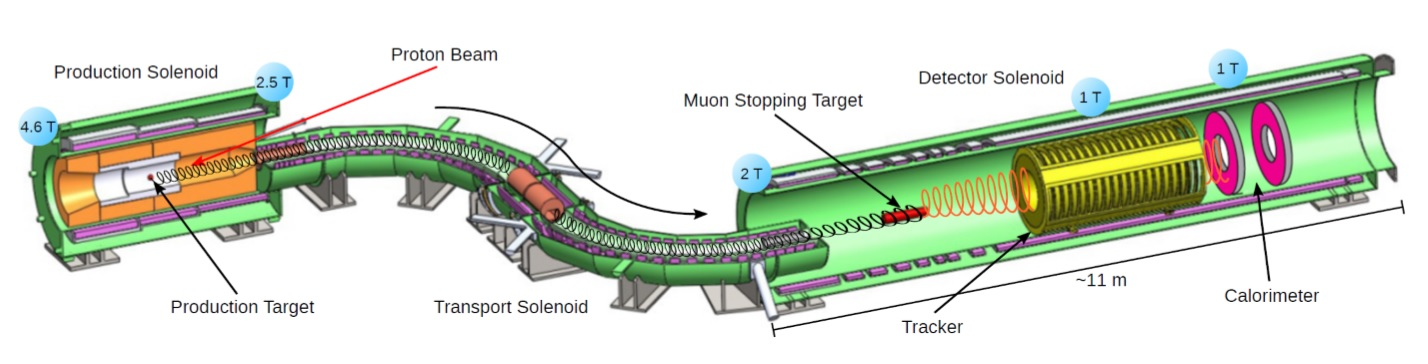
\includegraphics[scale=0.6]{mu2e_apparatus}\\
\caption[Mu2e apparatus]{Pictorial view of the Mu2e magnetic and detector systems \cite{Giovannella}.}
\label{_mu2e_apparatus_pre}
\end{figure}


\subsection{The Production Solenoid (PS)}
The Production Solenoid (Fig. \ref{_PS}) is the first part of the \textit{muon beam-line} (Fig. \ref{_MuonBeamline}) \cite{PS}. 
The production target is located in a graded magnetic field ($2.5 - 4.6$ T) that collects secondary particles produced when the proton microbunch strikes. The shape and position of both the target and the magnetic field have been optimized to maximize the production and collection of the desired particles: backwards pions and muons. 
The reason for using backwards produced particles is to avoid the overwhelming flux of particles 
(neutrons, photons, electrons and positrons from photon conversions) 
produced in the forward direction and the leftover incoming protons.\\
The 8 GeV pulsed proton beam enters from the low-field side and the magnetic field collects backward-produced pions towards the Transport Solenoid. 
Also a fraction of pions produced in the forward direction can be reflected by the gradient and  increase the pion yield. 
This is possible by exploiting the property of graded magnetic field often called \textit{magnetic mirror} 
and discussed previously in Sect. \ref{magnets}.

\begin{figure}[h!]
\centering
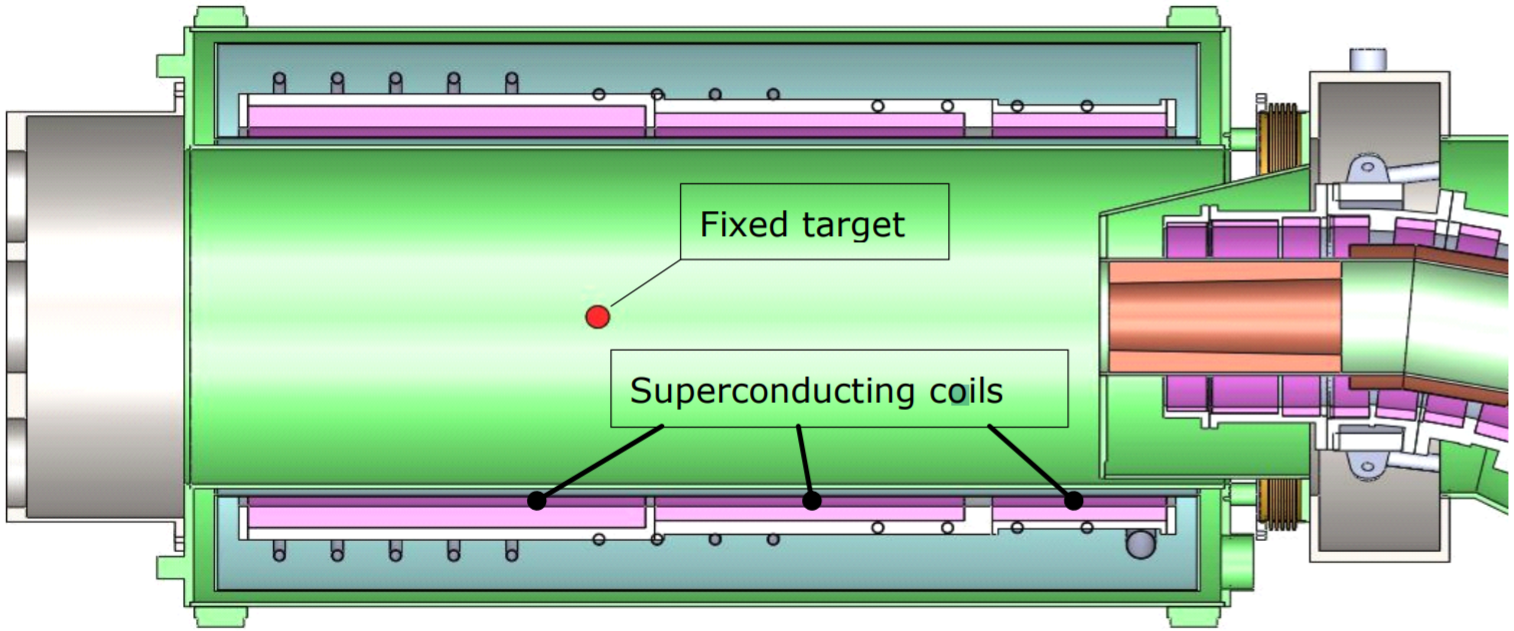
\includegraphics[scale=0.4]{PS}
\caption[Production Solenoid]{A section view of the Production Solenoid \cite{PS}. 
The incoming proton beam hits the target from the right, 
the next section of the beam-line (Transport Solenoid) is also on the right and the graded field collects particles towards it.}
\label{_PS}
\end{figure}

\paragraph{Production target}
The development of the production target has required a long optimization work and Fig.  \ref{_production_target_history} shows  the evolution of the design.
The solution chosen for the construction (last on the right in Fig.  \ref{_production_target_history}) is called Hayman-2 and is shown in Fig. \ref{_Hayman2}.
A high-Z material (tungsten) has been chosen to maximize pion production. 
The target has a cylindrical shape and is suspended in the central region of the production solenoid.
The right side of Fig. \ref{_Hayman2} shows the support structure.\\
To prevent material oxidation and increase the target lifetime, the device is operated in vacuum. 
The problem is that the target has to be suspended in vacuum and thus radiatively cooled.
The temperature is important for both the mechanical stress and the oxidation of the tungsten (which depends on the temperature and on the concentration of CO$_2$ and H$_2$O).
The solution to the first problem has been introducing a segmentation of the structure to reduce the thermal stress. 
Once the value of the vacuum has been set, the only way to further reduce the amount of oxidation is to reduce the temperature. 
The target shape has been optimized to maximize the emissivity while keeping the $\pi$/$\mu$ production as large as possible: this has been achieved by employing fins connected to each segment of the target (Fig. \ref{_Hayman2}).

\begin{figure}[h!]
\centering
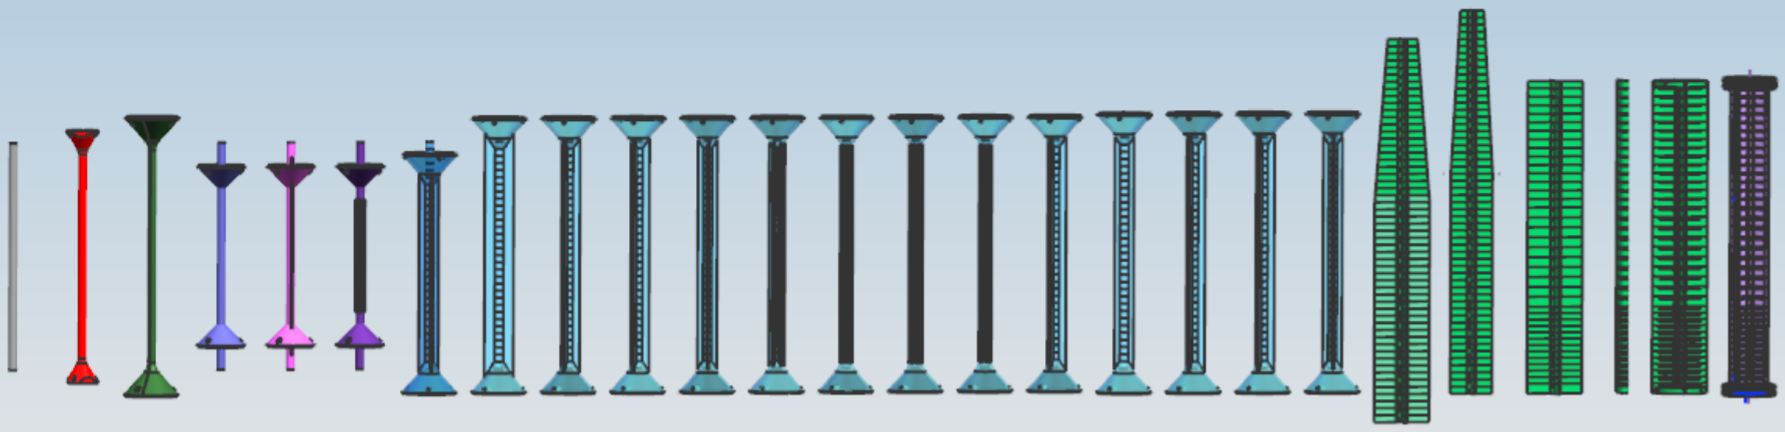
\includegraphics[scale=0.5]{production_target_history}
\caption[Production target history]{Evolution of the production target designs \cite{Pushka_Hayman2}. 
The most recent version, on the right, is called Hayman-2 and is shown in more detail in Fig. \ref{_Hayman2}.}
\label{_production_target_history}
\end{figure}

\begin{figure}[h!]
\centering
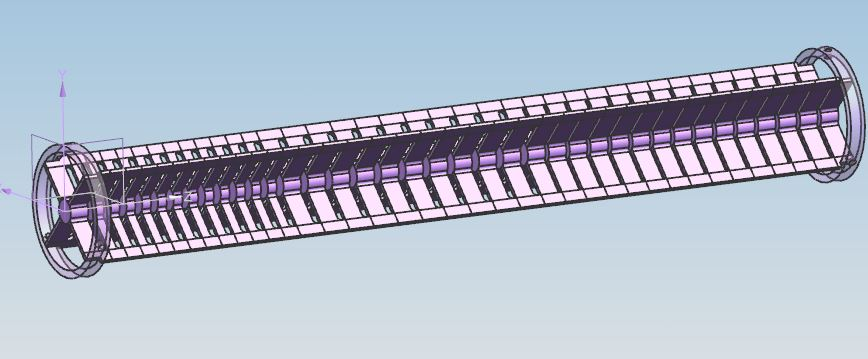
\includegraphics[scale=0.45]{Hayman2}\hfill
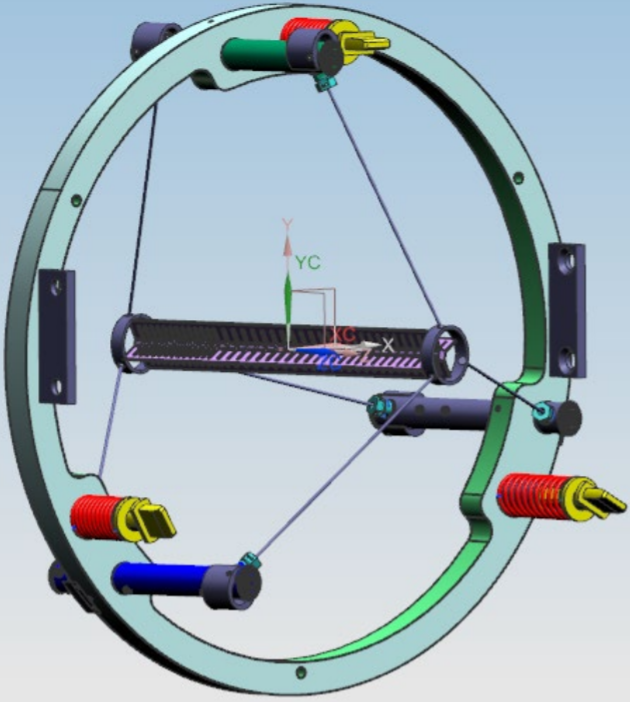
\includegraphics[scale=0.35]{Hayman2_structure}
\caption[Hayman2 stopping target]{On the left a closeup of the current design of the stopping target (Hayman-2 \cite{Pushka_Hayman2} \cite{bob_Hayman2}). 
It is interesting to notice the segmented structure and the presence of fins on every segment to allow the radiative cooling. 
On the right the design of the support for the Hayman-2 production target \cite{Pushka_Hayman2}.}
\label{_Hayman2}
\end{figure}

\subsection{The Transport Solenoid (TS)}
The gradient of the magnetic field in the Production Solenoid channels the particles towards the Transport Solenoid \cite{TS}. 
This section of the apparatus is a clever system that allows pions to decay before reaching the stopping target 
located in the Detector Solenoid
and performs a selection of the particles collected from the Production Solenoid. 
The Transport Solenoid is divided in 5 subsections, shown in Fig. \ref{_TS3}:
\begin{itemize}
\item TS1 and TS5 are the interfaces with the other sections and also contain a collimator to further reduce the backgrounds (like low momentum particles produced backwards in the PS and passing through TS1, or antiprotons which reach TS5 at the end of the transport system);
\item TS2 is a $\pi/2$ curved pipe in which the magnetic field performs a selection on the charged particles and their momentum. A bonus effect of the curved magnet is the separation in charge due to the drift discussed previously in \ref{magnets}; 
\item TS3 contains two collimators to exploit the cited feature of the TS2 to select particles of negative charge (left side of Fig. \ref{_TS3}). 
The two collimators are separated by a window to further reduce the presence of antiprotons;
\item TS4 is specular to TS2; it clears the beam from particles produced in the interaction with the TS3 while bringing the beam back on the plane of the experiment.
\end{itemize}

\paragraph{Antiproton window} As discussed in Sec. \ref{sec:antiprotons}, antiprotons produced in the production target can be collected and transported down to the stopping target. 
Photons created by $\pi^0$ resulting form antiprotons annihilation can convert asymmetrically and generate background electrons. 
The number of antiprotons can be reduced by the presence of collimators positioned at the interfaces between TS and the other two systems but there is also a specific window in the middle of the TS (between the TS3 collimators). 
This window has the specific function to stop antiprotons and the current design is a Titanium wedge (although still discussed against a Beryllium solution) \cite{PbarWindow}.

\begin{figure}[h!]
\centering
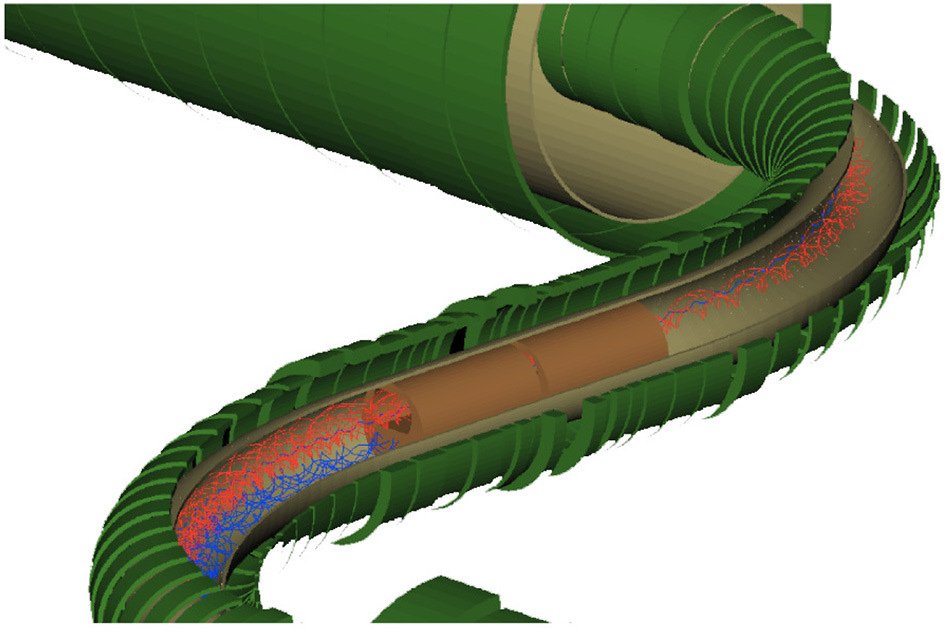
\includegraphics[scale=0.5]{MuonBeamline_TS_window_2} \hfill
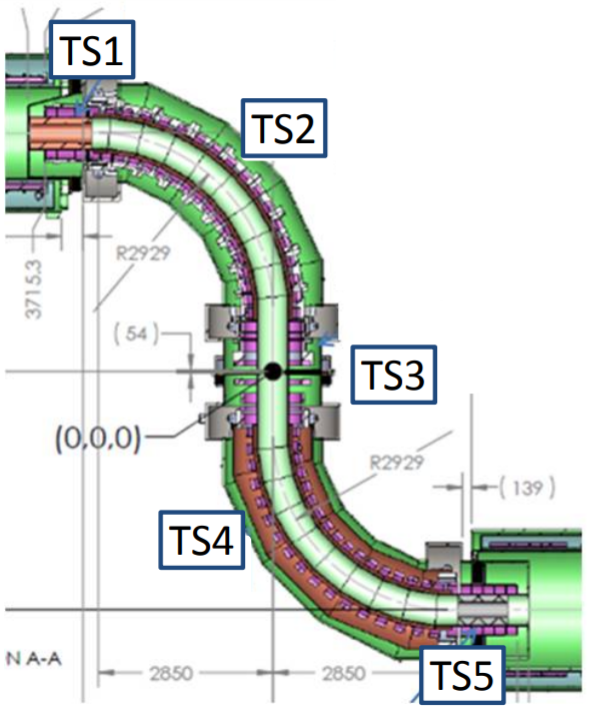
\includegraphics[scale=0.48]{MuonBeamline_TS_3}
\caption[Transport Solenoid]{A 3D view of the TS3 on the left \cite{bob_mu2e}. The particles traveling in the TS (moving left to right) are separated vertically in charge by the curving magnetic field and the TS3 collimators select the negative charged particles (red). 
On the right a schematic view of the Transport Solenoid sections described \cite{TS}.}
\label{_TS3}
\end{figure}

\subsection{The Detector Solenoid (DS)}
The Detector Solenoid (Fig. \ref{_DS}) is the last section of the muon beam line 
and contains the stopping target, the Mu2e detectors and a system of absorbers that surround the stopping target \cite{DS}.\\
The current estimate for collection and transport is  $1.6\times 10^{-3}\mu/$POT. 
Since approximately 40\% of muons will be stopped in the aluminum target, 
the rate of stopped muon is roughly $10^{10}\mu/$s. 
The magnetic field is graded near the stopping target (approximately linearly decreasing from 2 T to 1 T) 
to increase the acceptance for conversion electrons. 
Downstream this first section the magnetic field is approximately uniform.\\
In the following, we will describe the stopping target and the absorber system 
while the detectors will be the focus of the next Section.
\begin{figure}[h!]
\centering
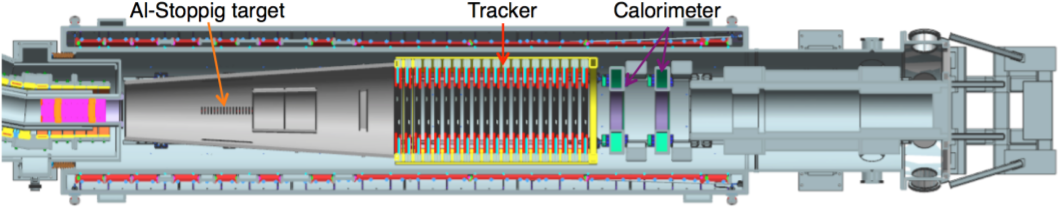
\includegraphics[scale=0.7]{DS_2}
\caption[Detector Solenoid]{Schematic depiction of the Detector Solenoid \cite{bob_mu2e}. 
The muons are incoming form the left, stop in the stopping target and the outgoing particles are detected by the Tracker and the Calorimeter, set downstream.}
\label{_DS}
\end{figure}

\paragraph{Stopping target} The target is required to be sufficiently massive to stop a large fraction of the incoming muons while letting the conversion electrons emerge. 
The risk with a too wide/massive target is a yield reduction and a momentum measurement degradation that would compromise 
the separation between signal and background. 
The current design is a suspended stack of $34\times100\ \mu$m Al foils with a hole in the center \cite{stopping_target}, 
shown in Fig. \ref{_stopping_target}.

\begin{figure}[h!]
\centering
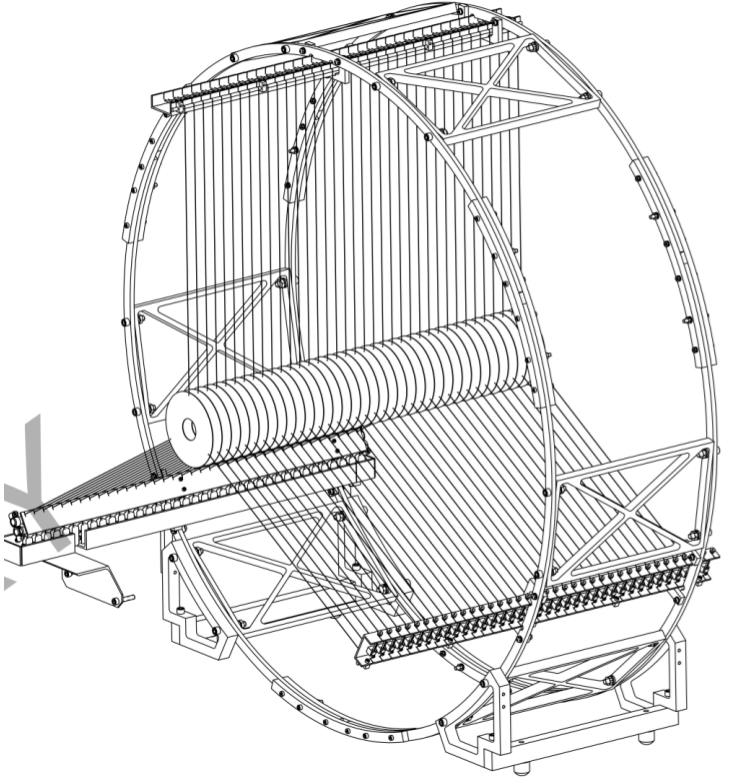
\includegraphics[scale=0.5]{stopping_target} %0.8
\caption[Stopping target support system]{The stopping target and its suspending infrastructure \cite{stopping_target}. The target is a stack of Al disks. The hole allows the reduce the interaction with not desired particles.}
\label{_stopping_target}
\end{figure}

\paragraph{Absorbers} As discussed in a previous section, 
particles ejected alongside electrons from the stopping target 
(neutrons, protons and deuteron from muon nuclear capture) 
can damage the detectors or increase the dead-time of the Cosmic Ray Veto. 
The stopping target is therefore surrounded by polyethylene absorbers \cite{stopping_target}
to reduce this effect. The system is composed of two structures 
named Inner and Outer Proton Absorber (Fig. \ref{_ProtonAbsorber}).

\begin{figure}[h!]
\centering
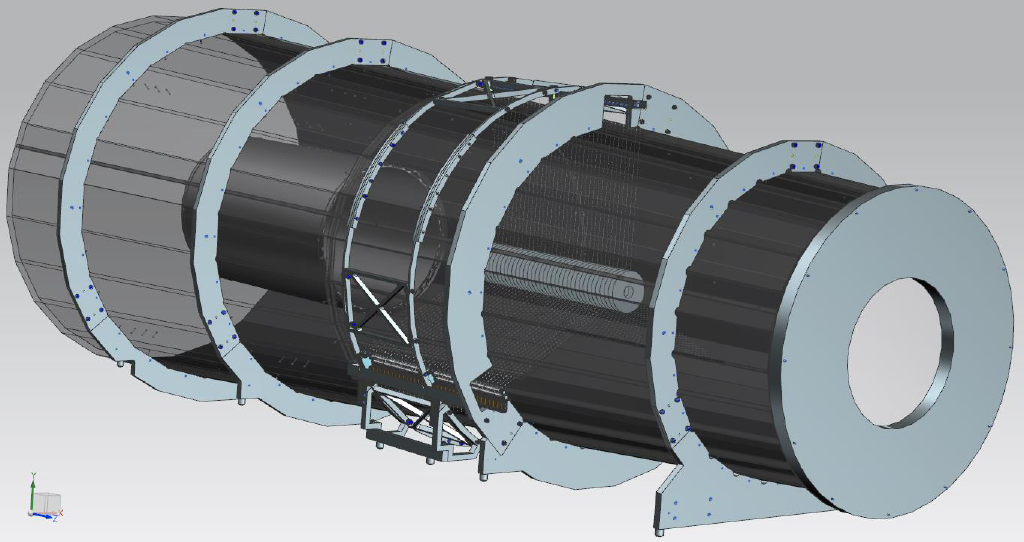
\includegraphics[scale=0.6]{ProtonAbsorber}
\caption[Proton absorber]{A schematic of the proton absorbers \cite{stopping_target}. 
This structure is needed to reduced the occupancy of the detectors and fake signals in the Cosmic Ray Veto: 
both can be due to particles ejected from nuclear captures in the stopping target.}
\label{_ProtonAbsorber}
\end{figure}


\section{The Mu2e detectors}
Mu2e employs a set of complementary detectors to measure particles momenta and energy.
The detectors are annular and are in a solenoidal field of about 1 T along the $z$-axis, in the
same direction of the muon beam. The annular design allows the passage of the overwhelming
flux of particles (i.e. products of muon capture, remnant beam, and electrons produced in the
initial proton collisions) that would generate excessive instantaneous detector occupancy and
accumulated radiation damage. Most decay muons are typically too low momentum to exit the
central region and never reach a detector element. 
This reduces the number of detector hits to a manageable level of occupancy. 
The Mu2e detectors consist of a straw-tracker followed by a calorimeter, surrounded by a cosmic ray veto.

\subsection{The Straw-Tracker}
The main function of the Mu2e tracker is to reconstruct particles trajectories. 
The simulation shows that a momentum resolution $<180$ keV$/c$ for 105 MeV electrons 
is necessary to provide the necessary separation between the conversion electron signal 
and the background due to the high end tail of the DIO spectrum. 
To minimize the energy loss in the detector and achieve this level of momentum resolution, 
a low mass tracker is required. Moreover, a high segmentation is necessary to 
handle the high particle rate and minimize the probability of pattern recognition errors
due to high detector occupancy.
The detector will be operated in a hostile environment due to the high level of radiation, 
for example and not only for the early burst beam-flash, and vacuum of the order of 10$^{-4}$ Torr.
This requires a detector with adequate thermo-mechanical robustness and timing performance.
The Mu2e Collaboration chose the straw-tube technology 
since it offers a remarkable compromise between low mass 
and excellent resolution \cite{Tracker:2016} \cite{Tracker:2018}.

\begin{figure}[h!]
\centering
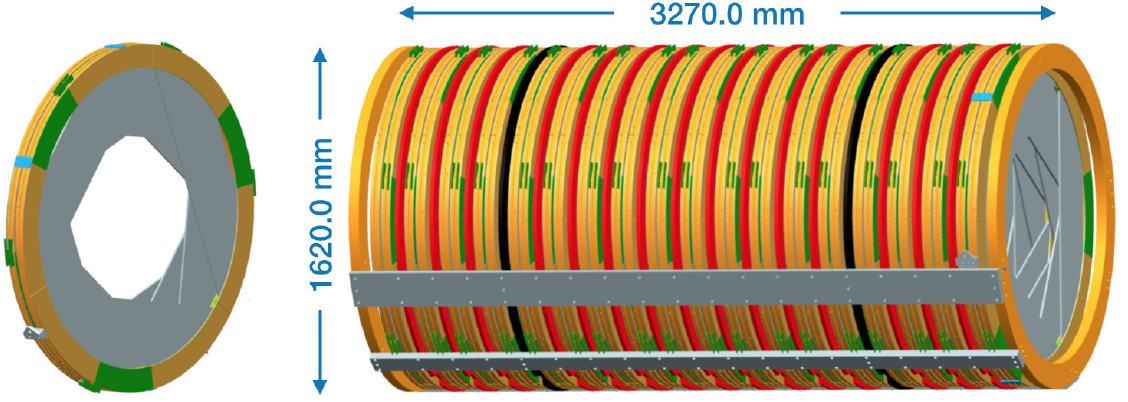
\includegraphics[scale=0.5]{Tracker_2}
\caption[Straw-tube tracker]{Geometry of the straw-tracker \cite{Manolis}. 
Straw tubes are mounted in two layers in a panel covering $120^\circ$ 
and 12 panels make a station, leaving the center with no detectors. The tracker is a series of 18 stations.}
\label{_tracker}
\end{figure}

%Timing wise in the structure of an event the current definition of signal window is 700 ns$<t<$1700 ns. In order to study the various %backgrounds, the Tracker needs to be fully operative on a larger time window, still under discussion but as of today set to be 500 %ns$<t<$1700 ns. While the higher value is simply defined by the arrival of a new micro-bunch, the lower is set to balance `workable' %occupancy and data collection.\\

\noindent
The annular geometry of the detector allows to reduce the occupancy due to low-momentum particles which are non-interesting and produce significant radiation damage.
The inner radius and the entire detector geometry have been determined through detailed 
simulation studies which 
have allowed to optimize the design in terms of occupancy, threshold of the momentum 
of tracks that can be reconstructed and momentum resolution (Fig. \ref{_tracker}).
The resulting momentum resolution for a simulated sample resembling the data expected after applying 
standard quality cuts is shown in Fig. \ref{_Tracker_resolution}.\\
The Mu2e Collaboration is continuously developing these studies as the detector simulation is improved and the prototypes are assembled, tested and characterized. The results of the tests run on a prototype are shown in Fig. \ref{_Tracker_prototype}.


\begin{figure}[h!]
\centering
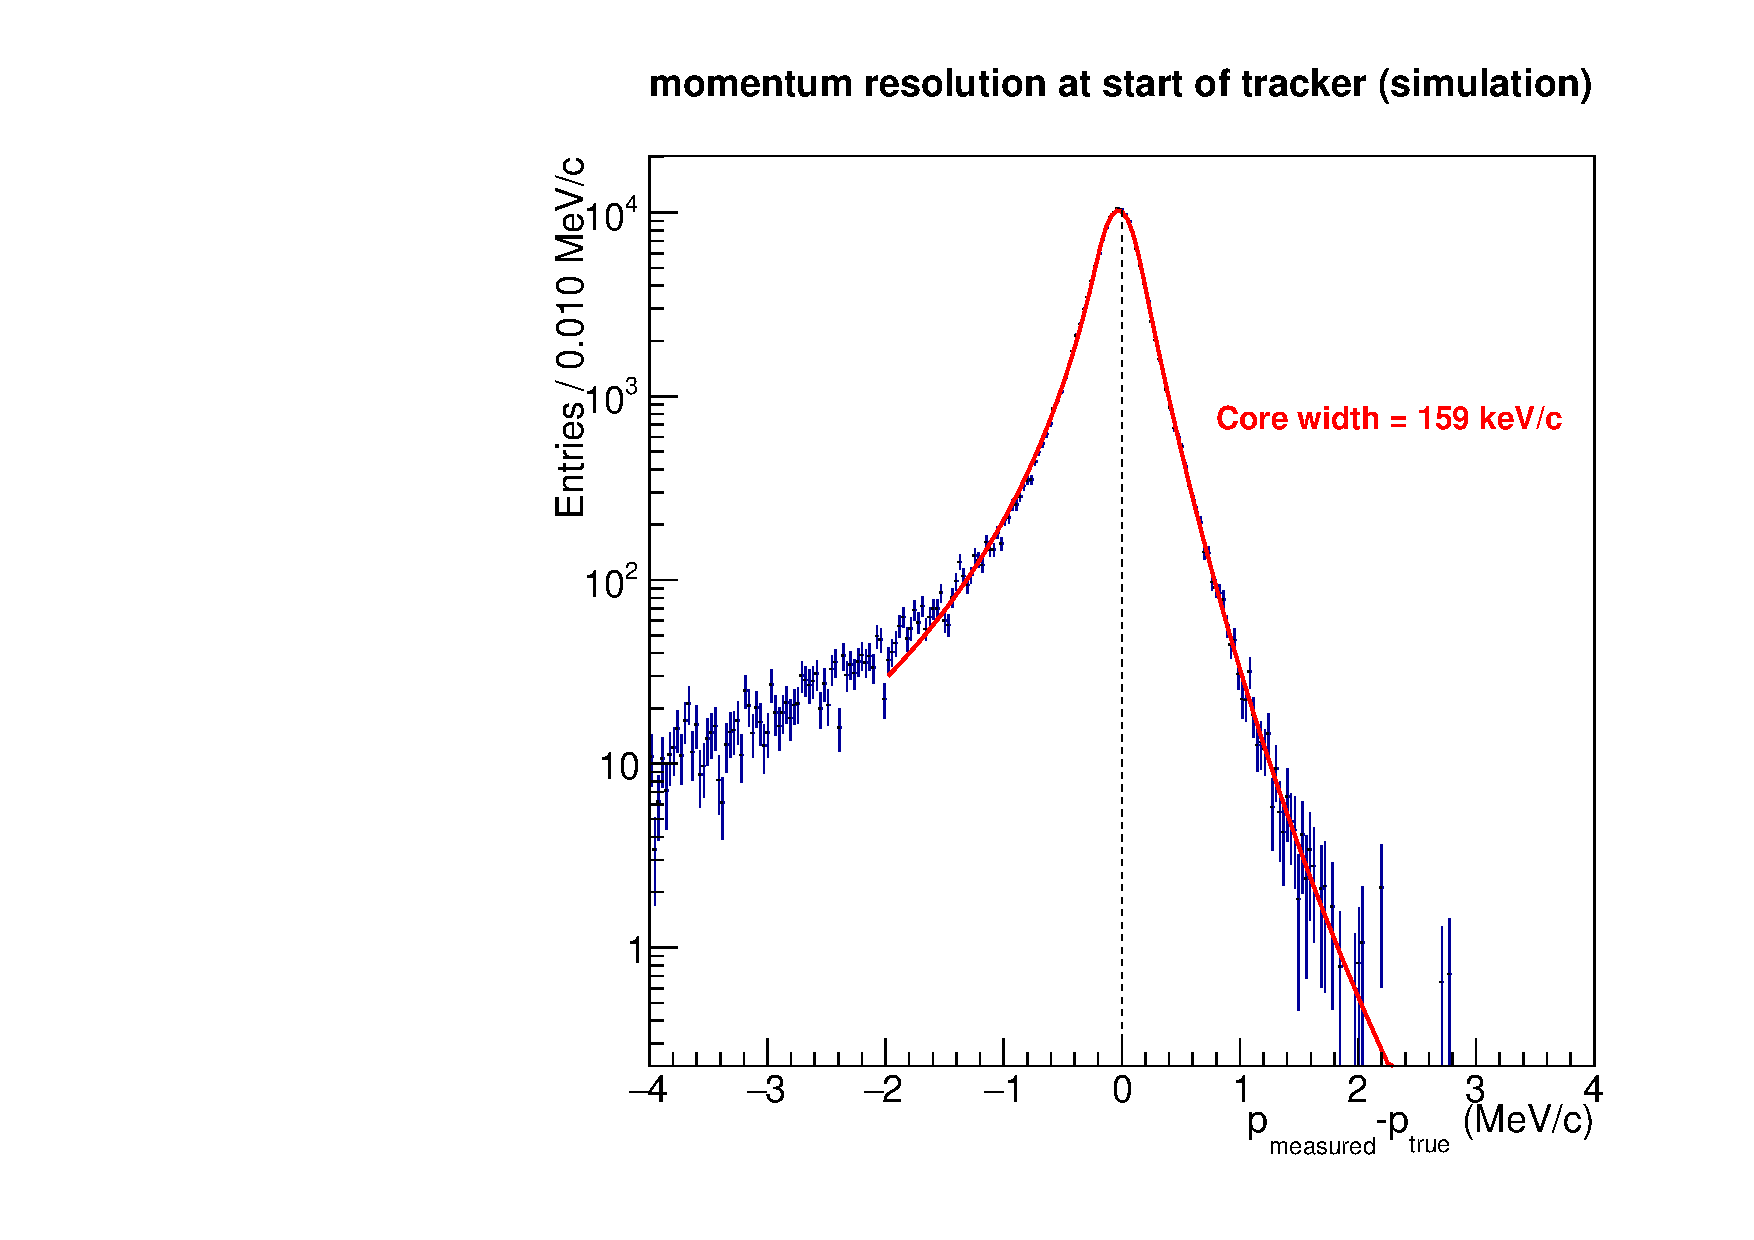
\includegraphics[scale=0.3]{Tracker_resolution}
\caption[Tracker simulated resolution]{Momentum resolution of the straw-tracker evaluated with  simulation. \cite{Giovannella}.}
\label{_Tracker_resolution}
\end{figure}

\begin{figure}[h!]
\centering
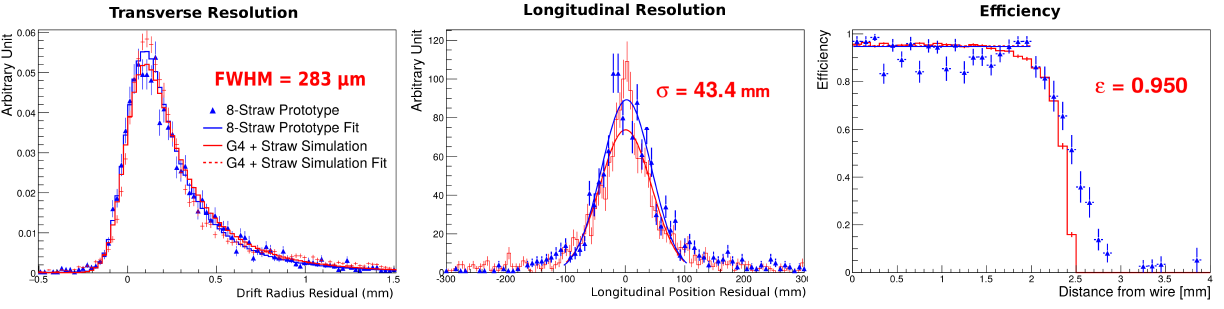
\includegraphics[scale=0.7]{Tracker_prototype}
\caption[Tracker prototype results]{Results of the tests of a 8 straws panel prototype tested with cosmic rays \cite{Giovannella}. 
From left to right: longitudinal and transverse resolution; efficiency.}
\label{_Tracker_prototype}
\end{figure}

\subsubsection{Straw-tracker structure}
The basic tracker element is named \textit{straw} and is made of 
a 25 $\mu$m gold plated tungsten sense wire centered in a 5 mm diameter, 
15 $\mu$m thick Mylar\textsuperscript\textregistered  tube  (Fig. \ref{_straw}). 
The straws are supported at both ends and their active length varies from a minimum of 334 mm to a maximum of 1,174 mm.
The drift gas is a 80:20 Argon:CO$_2$ mixture and the operating voltage is 1,500 V. The advantage of using straws
is that the detector can still be operated also in case of failure of single wires.
The inner surface of the Mylar tube has 500 \AA\ aluminum overlaid with 200 \AA\ gold as the cathode layer. 
The outer surface has 500 \AA\ of aluminum to act as an additional electrostatic shielding.\\

\noindent
Each straw is connected to a 4.95 mm diameter brass tube using silver epoxy.
As a protection from breakdown at the edge, an extruded kapton tube is placed inside the brass tube. 
An injection molded plastic insert is also placed inside the kapton tube. 
Attached to a groove in the insert a small, U-shaped, brass pin is placed. 
A 25 $\mu$m gold plated tungsten wire is soldered to the pin as well as epoxied to the plastic insert. 
Both brass parts are gold-plated to ensure good solder and epoxy joints.  \\
Groups of 96 straws are assembled in \textit{panels} that cover 120$^\circ$ and are made of two layers of straws 
to provide some redundancy and improve pattern recognition and track reconstruction
(Fig. \ref{_Tracker_panel_geom} \ref{_Tracker_panel}).
 A 1.25 mm gap between two consecutive straws in the same plane 
 provides sufficient mechanical tolerance for expansion; 
 the consequence of this design is that the straws need to be self supporting. 
 The readout of the straws is performed from both ends and the comparison 
 of the arrival time of the two signals allows to determine the hit position along the wire. 
 The resulting resolution on the hit position along the straw is approximately 3 cm. \\
A `full circle' is then made of 3 panels and it is called a \textit{face} (Fig. \ref{_Tracker_plane}). 
Two faces rotated  30$^\circ$ relative to each other constitute a \textit{plane}. 
Two planes are coupled to make a \textit{station}, mounting the second rotated on the vertical axes by 180$^\circ$. 
The whole tracker is a 3 m structure made of 18 stations  and employs a total of more than 20k straws. 
The inner and outer radii of the tracker are respectively 380 mm and 700 mm and have been determined 
to optimize the reconstruction efficiency for transverse momentum above 90 MeV$/c$; 
only $\mathcal{O}(10^{-12})$ of the DIO are expected to be reconstructable\cite{Manolis}. \\

\begin{figure}[h!]
\centering
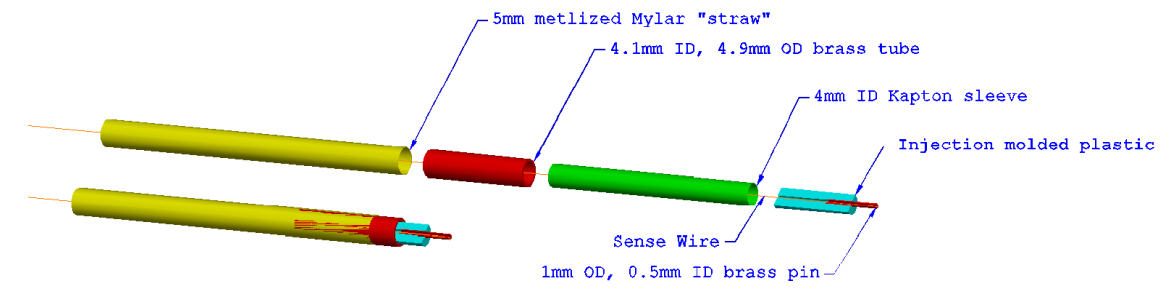
\includegraphics[scale=0.4]{straw}
\caption[Structure of a straw-tube]{The internal structure of a straw-tube \cite{MTDR}.}
\label{_straw}
\end{figure}

\begin{figure}[h!]
\centering
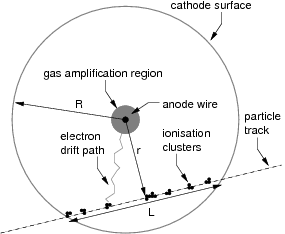
\includegraphics[scale=0.5]{straw_avalanche}
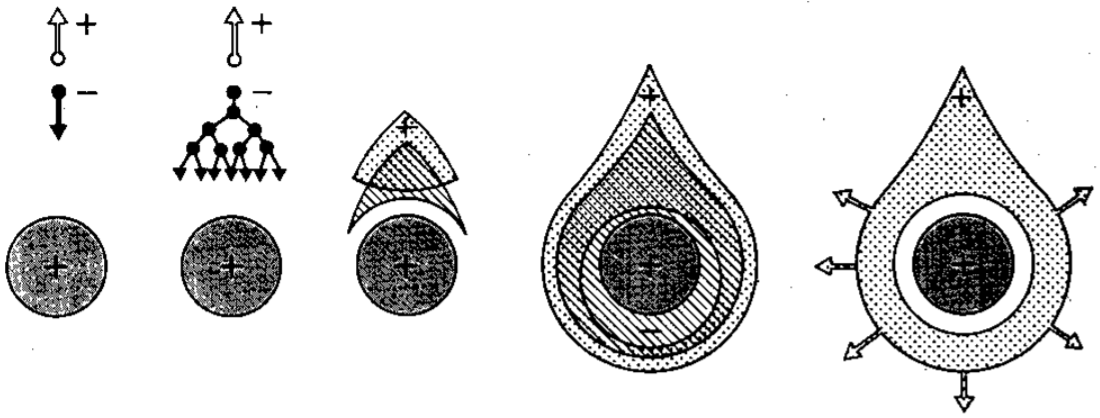
\includegraphics[scale=0.4]{straw_avalanche_2}
\caption[Avalanche process in straw-tube]{How does a stratube work \cite{MultiwireDrift} \textbf{[Useless?]}}
\label{_straw_avalanche}
\end{figure}

\begin{figure}[h!]
\centering
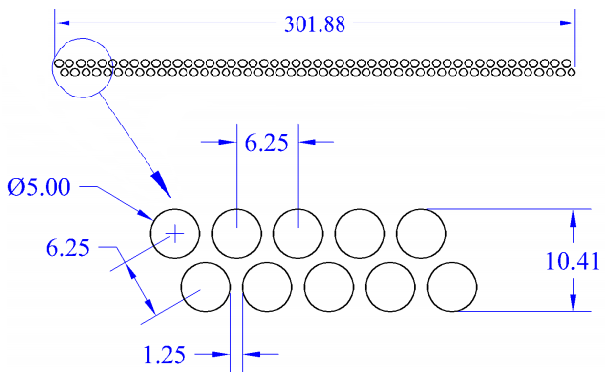
\includegraphics[scale=0.8]{Tracker_panel_geom}
\caption[Layout of straws in a panel]{Layout of the straws in a panel \cite{MTDR}. 
The distance between the straws is necessary to account for some expansion imperfections in the assembly. 
The two layers are staggered to have some redundancy and improve the reconstruction quality.}
\label{_Tracker_panel_geom}
\end{figure}

\begin{figure}[h!]
\centering
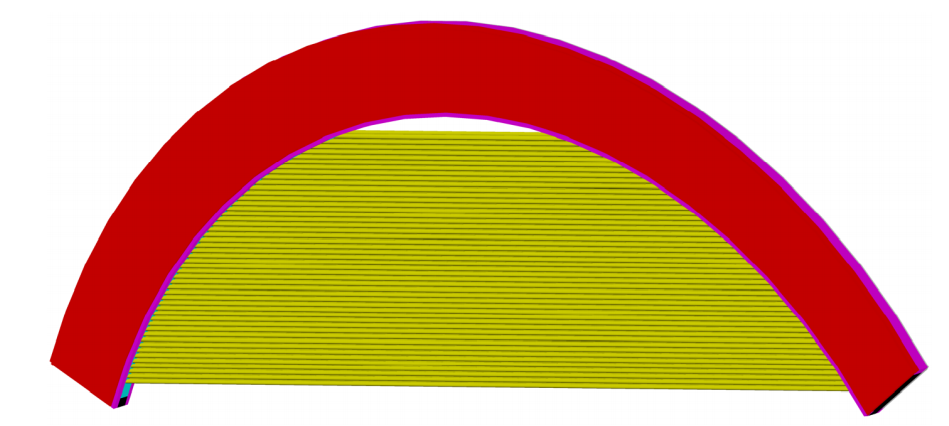
\includegraphics[scale=0.2]{Tracker_panel}
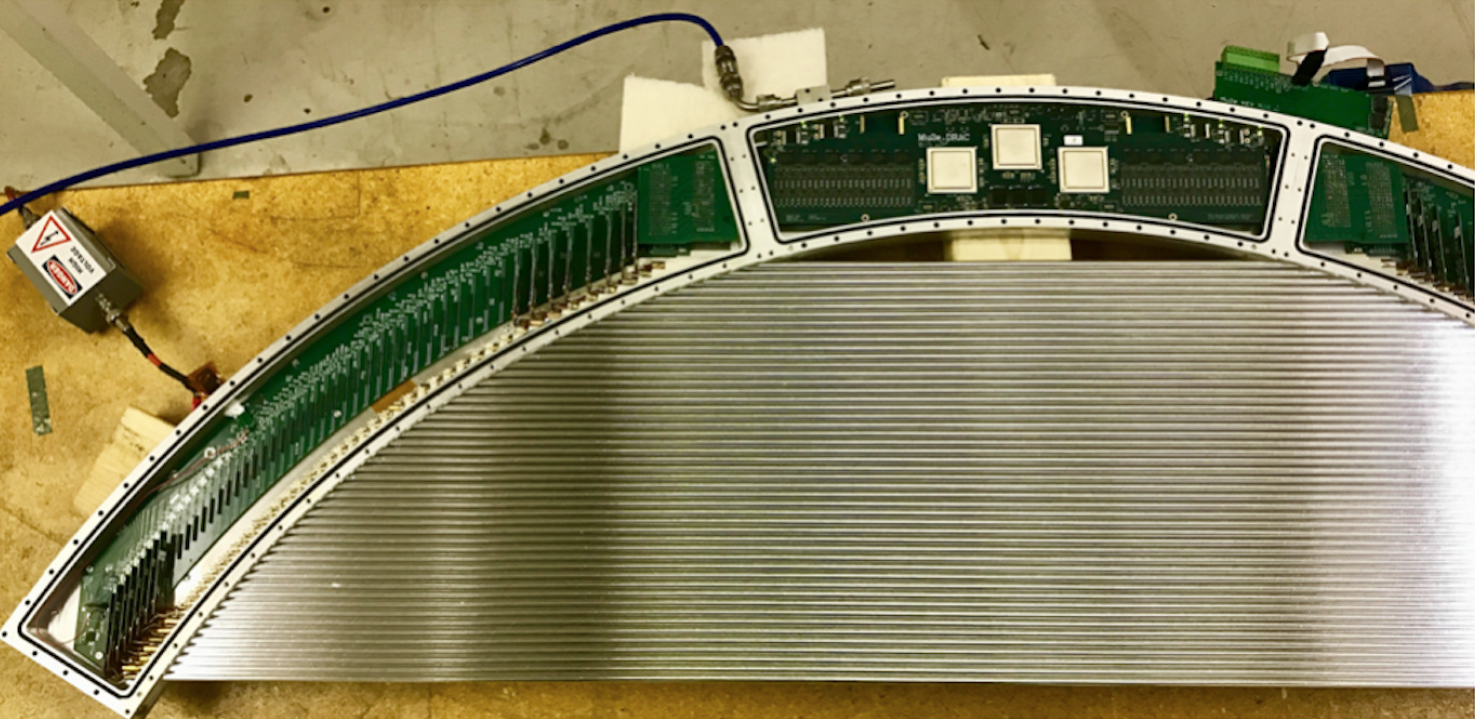
\includegraphics[scale=0.25]{Tracker_panel_picture}
\caption[A panel of the tracker]{Tracker panel \cite{MTDR} and a picture of an mounted panel with part of the electronics installed \cite{Manolis}.}
\label{_Tracker_panel}
\end{figure}

\begin{figure}[h!]
\centering
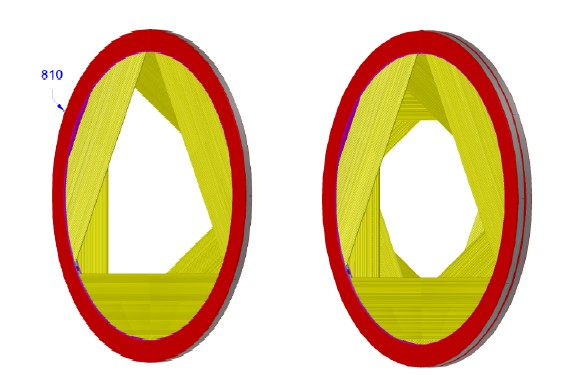
\includegraphics[scale=0.3]{Tracker_plane}
\includegraphics[scale=0.35]{Tracker_plane_picture}
\caption[Face and Plane of the tracker]{Tracker face and plane \cite{MTDR} and a picture of a mounted face with part of the electronics installed \cite{Manolis}.}
\label{_Tracker_plane}
\end{figure}


\subsubsection{Straw-tracker electronics}
The straw signals read out by the front-end electronics are amplified, 
digitized and transmitted to the Mu2e data acquisition system.
A schematic representation of the system architecture is reported
in Fig. \ref{_tracker_electronics}.
The front-end electronics (FEE) is installed directly on the detector 
to minimize unnecessary penetration of the cryostat and consists 
of the following sub-systems:
\begin{itemize}
\item High-voltage and low-voltage power lines;
\item The pre-amplification electronics that amplifies and transmits the raw straw signals to the digitizing system;
\item The digitizing system which processes the raw straw signals read from ends,  
computes two timing measurements and the total amplitude of the signal. 
The time difference between the signals at the two ends of the straw allows to compute the hit position along the 
wire;
\item The {\em Readout Controller} (ROC) receives the digitized data 
through Low-Voltage Differential Signaling (LVDS), to  minimize noise effects along the lines,
and provides the link between FEE and the Data Acquisition System.
\end{itemize}


\begin{figure}[h!]
\centering
\includegraphics[scale=0.4]{Tracker_electronics}
\caption[Straw-tracker electronics]{Signal flow for the readout of a straw from the detector to the Data Acquisition system \cite{MTDR}.}
\label{_tracker_electronics}
\end{figure}


\subsection{The Electromagnetic Calorimeter}
The calorimeter performs a number of fundamental functions complementary to the tracker, by providing particle identification capabilities, a fast online trigger filter and a seed for track reconstruction.
This detector (shown in Fig. \ref{_mu2e_calorimeter}) is once more cylindrical, with the characteristic hole, and made of two identical disks.

\noindent
Mu2e does not have a specific time stamp that identifies the interesting processes but rather a timing window in which the interesting they have to be identified. 
The consequence of this choice is that track reconstruction in the tracker begins from the coincidence in time of a number of hits. 
This implies that the track reconstruction algorithm has to be able to identify and remove the correlated background due to low momentum particles, for example $\delta$ electrons. 
This is currently performed by relying on a selection based on neural networks.
The calorimeter allows to reduce significantly the level of background by requiring also the presence of an energy cluster in the event (this point will be discussed in more detail in the following chapter, dedicated to the reconstruction).
The calorimeter information can be also employed to develop a standalone trigger to collect an unbiased sample of data useful to cross-check the performance of the primary trigger based on standalone tracker information.
Used as filter (Trigger) the Calorimeter will meet the requirement of rejecting the background by a factor $>200$ \cite{Calorimeter:2018}\cite{Donghia:2019}. The current estimate of the efficiency of this standalone trigger is 60-70 \%; enough for an unbiased crossed test of the tracking trigger efficiency.\\ 

\noindent
In the energy range of interest for Mu2e ($ \mathcal{O}(100$ MeV$)$) 
a total absorption homogeneous calorimeter 
provides a satisfactory performance. 
The alternative is normally between a liquid scintillator (for example Xe) or a scintillating crystal. 
The Mu2e collaboration opted for a crystal calorimeter and, 
after some R\&D with a number of materials (LYSO and BaF$_2$),
a more conservative and less expensive approach with Cesium Iodide (CsI) was chosen. 
The architecture of the detector is thus based on two hollow disks of CsI crystals read by 
Silicon PhotoMultipliers (SiPMs) (Fig. \ref{_mu2e_calorimeter}).\\ 
Since the position and time measured by the calorimeter are employed to provide a confirmation of the tracker measurements and help reject mis-reconstructed tracks due to spurious combinations of straw hits, the resolution on these quantities should be at the level the uncertainty on the extrapolated tracks. 
The energy and time resolution should also allow to perform particle identification to separate conversion electron candidates from cosmic ray muons. 
These requirements translate into the following resolutions: 
spatial resolution $\sigma_{x,y}<1$ cm; 
energy resolution $\sigma_E/E <10\%$; 
time resolution $\sigma_t < 500$ ps.
Moreover, the calorimeter has to provide this performance in a hostile environment
in terms of vacuum level, working condition of $10^{-4}$ Torr, 1 T plus an exposure to a total ionizing dose up to 15 krad/year and a neutron flux equivalent $10^{11}$ MeV/cm$^2$ \cite{Donghia:2019}.
A reduced-scale prototype of the calorimeter, made of a matrix of 51 CsI crystals and named Module-0, has been successfully developed, built and tested at INFN Laboratori Nazionali di Frascati and the measured performance in terms of resolution shown in Fig. \ref{_calorimeter_test} satisfy the original requirements.

\begin{figure}[h!]
\centering
\includegraphics[scale=0.5]{mu2e_calorimeter}
\includegraphics[scale=0.7]{mu2e_calorimeter_Module0}
\caption[Electromagnetic Calorimeter]{A 3D representation of the Calorimeter \cite{Calorimeter:2018}. The two disks have the same structure, shown in fig. \ref{_mu2e_calorimeter_disk}, and the electronics is mounted on the outside. On the right a picture of the Module-0, a working prototype \cite{Donghia:2019}.}
\label{_mu2e_calorimeter}
\end{figure}

\begin{figure}[h!]
\centering
\includegraphics[scale=0.5]{calorimeter_test}
\caption[Calorimeter prototype results]{Results of the test of the Module-0, a working prototype of the Calorimeter comprise of 51 crystals. \cite{Donghia:2019} \cite{Calorimeter:2020}}
\label{_calorimeter_test}
\end{figure}

%---------------

\subsubsection{Calorimeter mechanical structure}
Fig. \ref{_mu2e_calorimeter_disk} shows an exploded view of one calorimeter disk.
The internal and the external radii of the hollow cylinder are respectively 374 mm and 660 mm.
The internal support structure is made of carbon fiber to reduce the amount of passive material in the region 
where electrons are spiraling; 
the external structure needs to be sturdy enough to support the crystals and is made of aluminum. 
Each disk is comprised by 674 undoped staggered trapezoidal CsI crystals ($34\times34\times200$ mm$^3$  $\approx10.75\ X_0$). The crystals are wrapped with 8 layers of 25 $\mu$m Tyvek\textsuperscript \textregistered film to maximize the light transport and minimize the crass-talk. \\
The two structural cylinders are connected by two plates:
\begin{itemize}
\item The Front Source Plate is made of carbon fiber to reduce the energy deposit 
and accommodates the calibration circuit, were a radioactive fluid flows;
\item The downstream plate supports the SiPMs the front-end electronics and the cooling system. 
The plate is made of PolyEther Ether Ketone (PEEK) primarily for the low outgassing rate and thermal conductivity of the material.
\end{itemize} 
The separation between the two disks ($\approx 70$ cm) has been chosen to be so that if a 105 MeV particles travels trough the hole of the upstream disk, it will hit the crystal surface of the downstream one.\\
On the external surface of each cylinder 10 \textit{Digital Acquisition }(DAQ) \textit{crates} 
host a number of electronic boards.
Each crate hosts 8 boards tat provide the power supply to the front-end electronics and SiPM,
perform the digitization of the SiPM analog data and transmit the digitized data do the Mu2e 
Global Data Acquisition System.

\begin{figure}[h!]
\centering
\includegraphics[scale=0.8]{mu2e_calorimeter_disk_2}
\caption[Disk of the calorimeter]{Structure of one of the two disk of the Calorimeter and picture of some prototype for the SiPM integration \cite{Calorimeter:2020}.}
\label{_mu2e_calorimeter_disk}
\end{figure}


\subsubsection{Calorimeter electronics}
Each CsI crystal is paired with two HAMAMATSU SiPMs that convert the scintillation light
into an electric signal. 
Two full-custom electronic boards complete the front-end electronics system
and supply the power to the SiPMs, amplify and transmit the SiPM signals to the digitization boards
hosted in the DAQ crates. 
The reason to use two SiPMs for each crystal, for a total of 1348 SiPM/disk, 
is to minimize the efficiency loss if one SiPM should fail and thus increase the entire readout
system robustness.\\ 
%Two chips (Amp-HV) are connected to the back of the SiPMs and provide amplification and regulation of the bias voltage \ref{_mu2e_calorimeter_disk}. Group of 16 Amp-VH are controlled by one ARM (?) controller, placed on one interface board located in the DAQ crate. This board distributes and regulates both high and low voltage.\\ \\
%The analog signals coming from the FEE are transmitted to the data acquisition boards, hosted in the DAQ crates. 
The main function of the digitization boards named  \textit{Digitizer ReAdout Controller} (DIRAC) 
is to digitize the SiPM analog signals and transmit the digitized data to the Mu2e Data Acquisitiomn System.
Additional boards necessary to distribute power, monitor photo-sensors and front-end electronics  performance, 
are called \textit{Interface Boards}. 
As anticipated, there are 10 DAQ crates per disk, and each crate hosts 8 DIRAC and 8 Interface Boards. 
We report only a brief description of the components employed on the DIRAC:
\begin{itemize}
\item 10 Analog to Digital Converters (ADC) to  digitize the SiPM analog signals received 
from the front-end electronics;
\item 1 Field Programmable Gate Array (FPGA) to processe the digitized data received from  
the Analog to Digital Converters (ADC);
\item 4 DC-DC converters to generate the voltage levels required by the several components 
mounted on the boards from the voltages received from the external power supply; 
\item 6 Linear Regulators to provide low voltage high current outputs with high precision;
\item A Jitter Cleaner to generate a clean and stable clock signal necessary for the ADCs and FPGA optimal performance.
\end{itemize}
In coincidence with each DIRAC board, there is also one Interface Board that hosts an ARM controller 
and voltage regulators to provide the power and monitor the performance of the front-end electronics.

\subsection{The Cosmic Ray Veto}
Cosmic Rays represent one of the most significant sources of background to the conversion electron search.
Mu2e thus needs a dedicated veto system \cite{CRV:2019} to cover most of the experiment 
(up to the Transport Solenoid, as shown in fig. \ref{_CRV}) and reduce the contamination due to muons traversing the detector area 
and to particles collected by the magnetic system and transported down to the Detector Solenoid. 
A problem for the veto performance derives from the large neutron flux generated 
in the Production Target that can produce a large occupancy and a significant dead-time and thus reduce the efficiency
of Mu2e data-taking. To minimize this effect, large concrete blocks are employed to shield the volume of the Detector Solenoid.\\
The veto is made of extruded scintillator counters with embedded wavelength-shifting fibers.
This technology is relatively cheap, robust, uncomplicated and requires limited maintenance, 
although scintillator ageing and the resulting performance decay can be a problem for a
data taking planned to last for a few years.
Each counter is read by one or two SiPMs depending on the position in the detector. 
The entire veto requires approximately 1248 m$^2$ of scintillator and 50 km of fiber. 
Scintillator counters will be grouped in more than 80 modules with requirements that will depend on the position.
The section of the detector is shown in Fig. \ref{_CRV_module_geometry}.
The modules will be composed of four layer of staggered counters. 
Fig. \ref{_CRV_module_geometry} shows also the readout electronics. 
The simulation shows that requirement to have the coincidence of at least 3 hits in 4 layers
identifies muons with the efficiency of 99.99\% which is fully satisfactory for Mu2e performance.


\begin{figure}[h!]
\centering
\includegraphics[scale=2]{CRV}
\caption[Cosmic Rays Veto system]{Overview of the Mu2e apparatus enclosed by the 
Cosmic Ray Veto \cite{CRV:2019}. 
The Veto covers the Detector Solenoid and part of the 
Transport Solenoid to avoid Cosmi Rays collected in the junction 
between the two and transported in the Detector Solenoid by the magnetic fields.}
\label{_CRV}
\end{figure}

\begin{figure}[h!]
\centering
\includegraphics[scale=0.6]{CRV_module_geometry}
\includegraphics[scale=0.4]{CRV_module_components}
\caption[Cosmic Rays Veto system: section and electronics]{Section of the CRV (Left) and readout electronics (Right) \cite{CRV:2019}.}
\label{_CRV_module_geometry}
\end{figure}

\subsection{The Trigger and Data Acquisition System}
A crucial part of any experiment is data collection, filtering and storage. 
In Mu2e the detector signals are amplified and digitized by the electronic systems which reside 
on the detectors and are then processed online by the Trigger and Data Acquisition (TDAQ)\cite{TDAQ}. 
This TDAQ provides the hardware and software tools to store and combine the digitized data. 
The primary function is to apply online filters to reduce the overall flux of data 
selected for permanent storage and offline analysis. 
The logical structure of this system is shown in Fig. \ref{_TDAQ}.

\begin{figure}[h!]
\centering
\includegraphics[scale=0.6]{TDAQ}
\caption[Trigger and Data Acquisition System]{Schematic representation of the Trigger and Data Acquisition System architecture \cite{TDAQ}.}
\label{_TDAQ}
\end{figure}

\section{The monitor of the stopped muon flux}
%\subsection{Stopped muons and photons}
The goal of the Mu2e experiment is to measure the ratio between the muon conversion and the nuclear capture rates
($R_{\mu e}$) in the Al target. 
There are a number of possible ways to measure the total number of stopped muons and determine 
the denominator of this ratio.
A measurement done upstream with respect to the muon stops would rely on the estimates for particle collection and propagation in the apparatus. 
A more reliable solutions thus is to exploit direct measurements of the particles resulting from the processes a stopped muon can undergo.
The choice is counting photons generated by specific physics processes involving the muonic atoms and nuclear capture.
 
\subsection{Baseline Mu2e design: measuring the muon beam flux}
Once a muon has been stopped in the target and the muonic atom has been formed, photons can be produced in a number processes. 
The different processes generate photons of different energies and the spectrum has been measured in Al by the AlCap Collaboration \cite{AlCap:2015}\cite{AlCap:2020}.
Fig. \ref{_HPG_Spectra} shows the energy spectra of prompt (red line) and delayed (green line) photons.
The three highlighted energies correspond to three different physics processes:
\begin{itemize}
\item Muonic X-rays with the energy of 347 keV are produced when the muonic atom system cascades $2p\rightarrow 1s$; 
the process is prompt;
\item Gammas with the energy of 1809 keV are produced by the decay of excited Mg nuclei and this process is also prompt:\\
$\mu^-+\ _{13}^{27}$Al$\rightarrow \ _{12}^{26}$Mg$^*+n\nu_\mu$; $\ _{12}^{26}$Mg$*\rightarrow \ _{12}^{26}$Mg$+\gamma(1809$ keV$)$;
\item Gammas with the energy of 844 keV are generated in the decay of long-lived isotopes produced by the capture, this is not prompt $\tau_{1/2}\approx9.5$ min:\\
$\mu^-+\ _{13}^{27}$Al$\rightarrow \ _{12}^{27}$Mg$+\nu_\mu$; $\ _{12}^{27}$Mg$\rightarrow \ _{13}^{27}$Al$+\gamma(844$ keV$)+e^-+\overline{\nu}_\mu$;\\
\end{itemize}

\begin{figure}[h!]
\centering
\includegraphics[scale=0.6]{HPG_Spectra}
\caption[Photons spectrum from stopped muons]{Prompt (red line) and delayed (green line)  
photon spectra in Al measured by the AlCap Collaboration.}
\label{_HPG_Spectra}
\end{figure}

\noindent
High Purity Germanium (HPGe) detectors have sufficient energy resolution to measure the 347 keV and 844 keV lines. 
The drawback with HPGe detectors is that they are slow and susceptible to radiation damage due to neutrons which
are abundantly produced in Mu2e.
The solution adopted by Mu2e is to move the system away from the source (i.e. the Al stopping target) and
reduce the rate by $1/r^2$. 
The final design is still under development but the detector will be placed at approximately 35 m from the stopping target and adequately shielded \cite{STM:2016}. 
On the other hand, a Cesium doped Lanthanum(III) Bromide (LaBr$_3$(Ce)) detector would have a lower energy resolution but a much higher rate capability and resistance to radiation and would allow to measure the 1809 keV line \cite{LaBr3:2020}.\\
The geometry of the Stopping Target Monitor, comprised of these two complementary systems, is still under study. 
Several alternative solutions for the orientation and shielding are possible and Fig. \ref{_STM_geom} shows one possible configuration.

\begin{figure}[h!]
\centering
\includegraphics[scale=0.6]{STM_geom}
\caption[Geometry of the Stopping Target Monitor]{Geometry of the Stopping Target Monitor.}
\label{_STM_geom}
\end{figure}

\noindent
We should notice at this point that the time necessary to measure 
the stopped muon flux is a key parameter if we have to develop a monitor of the muon beam, 
since the beam intensity fluctuations, which have a significant impact
of the detectors performance, can occur on the millisecond timescale (Sect. \ref{_Fluctuations}).
The problem with the HPGe detector is that its time response is not
sufficiently fast to measure beam intensity variations on this timescale. 
On the other hand, 
while the LaBr$_3$(Ce) detector would be sufficiently fast, 
the problem in this case is the low rate of $\gamma(1809)$ keV.
The up to date estimate of the rate suggests that using this system the measurement of the flux will be done at $10\%$ integrating over $2\div3$ supercycles \cite{LaBr3:2019}.
As discussed in Sec. \ref{sec:beam}, this translate to a time scale of $\approx 3.5$ s.
To conclude, both solutions currently adopted by Mu2e for photon counting provide a good overall estimate of the averaged muon flux but cannot provide a monitor on the millisecond timescale, that is the timescale 
of the expected intensity fluctuations (Sec. \ref{_Fluctuations}).
Developing a solution for this problem has been the main topic of this Thesis.


\subsection{This Thesis: monitoring the muon beam intensity fluctuations on the millisecond timescale}
Our idea is to exploit protons and deuterons ejected after muon nuclear captures in the Al target
to monitor the fluctuations of the muon beam intensity and, consequently, of the proton beam intensity 
which occur on the millisecond timescale due to the resonant extraction procedure.
The method heavily relies on the proton and deuteron track reconstruction in the straw tracker
and will be thoroughly described in the following Chapters.\\ 
The reason why we consider only beam fluctuations and not the total muon flux is 
because proton and deuteron ejection after muon nuclear capture is still a relatively poorly understood process
and, for the moment, it would be hard to perform absolute measurements.  \\
As already discussed, although the $\gamma$-counting techniques will not have the possibility 
to evaluate on a short time period the fluctuation of the number of stopped muons or of the proton beam intensity, 
the joint effort of proton and photon counting could give us both the necessary uncertainty of the total normalization 
and a good understanding on the underlying beam timing structure.



\section{Simulation and Analysis tools}
\subsection{\textit{art} and .fcl}
The Mu2e simulation and analysis tools revolve around the joint use of two pieces of software (other than the C++/ROOT analysis macros): the \textit{art} framework and the FHiCL files. Here we give a short definition of both but even an introduction would be out of scope. This section is based primarily on the documentation/tutorials available on the  \href{https://mu2ewiki.fnal.gov/}{Mu2eWiki} and in the "art workbook"\cite{art}.

\paragraph{\textit{art}} The first piece of software is an event processing framework, written in C++ and developed by the Fermilab Scientific Computing Division. It provides the functionalities of common usage (I/O, database access, ... ), but its core feature is to be modular: physics algorithms are developed as plug-in modules. 
This feature allows maintaining a single common framework, while every collaboration develops its own modules. 
It is common to use the term \textit{job} to indicate the running of a sequence of modules.   
Every module is a C++ class which inherit from one of the module base classes defined by \textit{art} (EDAnalyzer, EDProducer or EDFilter). The modules are then compiled and \textit{art} loads the shared libraries as plugin.

\paragraph{FHiCL} The configuration files for \textit{art}-jobs are written in the Fermilab Hierarchical Configuration Language (FHiCL with the extension .fcl) and are the direct interface to the software for many physicists. 
Most of the common tasks are faced defining in a configuration file which modules of the simulation/analysis are needed, and setting the necessaries parameters. 
Although that is the final design,the
currently fast evolution of the modules, is not yet uncommon to encounter the necessity of open single modules for the debugging procedure or to introduce ad hoc functions or minor modification.\\ \\
At my arrival, most of the existing modules of the Mu2e reconstruction had been developed with the explicit (or implicit) intent to search for conversion electrons: for this study on proton hits and tracks reconstruction, the necessity to sift through the modules was encountered on a daily basis. 
Although I didn't develop new modules myself, I needed a good understanding of their structure and interplay and I applied numerous changes or fixed several bugs.

\subsection{STNTUPLE}
One of the plug-in modules for \textit{art} is specific to the usage of the STNTUPLE \cite{stntuple}\cite{stntuple:giani}.
These are both a \textit{n}-tuple data format and a light-weight \textit{n}-tuple analysis framework, written (almost) exclusively in C++. 
This type of data structure was used in CDF for many years and then ported to Mu2e. 
Every STNTUPLE ROOT file contains multiple branches, each corresponding to a data block: these are containers for Mu2e raw and/or reconstructed data. 
Using the appropriate module in the .fcl \textit{art}-job configuration file, a STNTUPLE of the data produced during the running is created and stored. 
What type of data is saved in this format is clearly customizable.\\
After the .stn file is generated, invoking the necessary module allows to run every analysis on this data format, avoiding the re-running the reconstruction. Cardinal in this workflow is that the user analysis packages requires almost no I/O infrastructure beacuse the loop on the events is performed by the STNTUPLE framework itself.

\begin{figure}[h!]
\centering
\includegraphics[scale=0.8]{mu2e_datahandling}
\caption[Mu2e data handling]{Both generation and reconstruction of events are done through \textit{art}-jobs configured using FHiCLs and importing the necessary C++ modules. 
Other modules, like the Event Display and TAnaDump are used, are used for debugging purpose.
The analysis workflow relies on the usage of STNTUPLE.}
\label{_mu2e_datahandling}
\end{figure}



%---------------------%---------------------
%---------------------%---------------------
%---------------------
\chapter{Track reconstruction in Mu2e}
{\itshape This Chapter is dedicated to the description of the track reconstruction algorithms employed in Mu2e. 
The algorithms and the  code have been conceived with the primary purpose 
to reconstruct electrons in the energy range of the conversion electrons 
and a number of user-defined parameters are set by default to the values optimized for this  case.
For alternative or more specifc applications, for example reconstructing proton tracks, 
a further optimization of these parameters has to be performed by the user
on a case-by-case basis.
These non-standard applications are being developed by the 
Simulation Group and, in this respect, this Thesis is a pioneering work.
This Chapter is also my contribution to the effort of providing 
useful reference to the Collaboration and improve the
already available documentation dedicated to the problem of track reconstruction in Mu2e \cite{GianiPatRec:2016}, \cite{GianiPatRec:2020}, \cite{Brown:2014}, \cite{Kalman},  \cite{KutschkePaper}.}

\section{Hits reconstruction and pre-filtering}
\subsection{Straw tracker hits}
Charged particles traversing the tracker volume generate ionisation charge in the gas enclosed by the straw which is collected and produces electric signals.
Since the straws are readout by the front-end electronics from both sides, 
the first step in the hit reconstruction process is combining the two resulting electric signals 
to estimate the hit time and position `along the wire'. 
In the reconstruction code, this information is stored in an object conventionally named \textit{StrawHit}.\\
The most challenging problem with track reconstruction in Mu2e 
is that a multitude of StrawHits are commonly found
in the  $1.7\ \mu$s time window corresponding to an event.
The first crucial task is thus identifying the StrawHits close in time that could have been generated by the same particle traversing the tracker.
To improve hit spatial resolution and reduce the possible combinatorics when searching for tracks, 
adjacent StrawHits in a panel\footnote{As reported in Chapter 2, a panel is made of two layers of straws.}, 
which are most likely due to the same particle, 
are combined in a more complex object named \textit{ComboHit}. 
While preserving the information of the single StrawHit, the ComboHit provides the average time and position of the cluster. 
Unfortunately, this process is complicated by the presence of many hits produced by low energy (of the order of few MeV) electrons knocked out by Compton scattering. 
These electrons, commonly named $\delta$-electrons, follow small-radii trajectories and can generate numerous hits all contained in a limited portion of volume that, consequently, shows a high occupancy. 
This effect is mitigated by the fact that patterns of hits generated by $\delta$-electrons are significantly different from those generated by particles in the energy rangeof interest of Mu2e and can be identified by employing \textit{Multi Variate Analysis} 
(MVA\footnote{The description of a multivariate analysis is outside the scope of this work and so is the process of MVA-training. Since these techniques are fundamental for the background flagging, we will briefly describe the basic principles.
When looking for patterns in a multi-variable space, it is a common procedure to define a set of statistical models that examine the variables measured and estimate the probability that these are compatible with the pattern. 
Once the variables have been chosen, the MVA is trained to recognize patterns by looking at examples known to the trainer and a feedback can be provided to improve the identification.\\
When looking for $\delta$-electrons, the most significant variables are the position and spread of the ComboHit, both in the $XY$ plane and in the $Z$ direction.}) algorithms.\\
At this level of the reconstruction process, the information provided by the tracker has been translated in a collection of ComboHits, resulting of the combination of a list of associated StrawHits and specified by its time and position.
The clustering algorithm also allows to identify and  performs a partial reduction and filtering of the background hits due to secondary electrons.

\subsection{Electromagnetic calorimeter hits} 
The logical equivalent of a ComboHit in the tracker is named \textit{Cluster} in the calorimeter and it is the combination of the signals generated in a group of crystals by a particle hitting the detector \cite{CalCluster_2} \cite{CalCluster}. 
The Cluster is reconstructed starting from the crystal with the highest energy deposit and adding all the adjacent crystals with a signal within a 2 ns window and with an energy above a programmable threshold. 
The process is then iterated starting from the added crystals until there are no more crystals to be added.
Given the accuracy of the time measurement provided by the calorimeter, the Cluster time measurement can be exploited to determine a window in which all the ComboHits generated by a particle traversing the tracker should be located.
The calorimeter thus performs a precious role in providing a seed for pattern recognition that reduces significantly the combinatorial background in the tracker.

\section{Finding the helices}
The goal of the Mu2e tracking software is reconstructing the tracks generated by charged particles traveling in the Detector Solenoid magnetic field and, as discussed in \ref{magnets}, 
the trajectories they follow would be helices if no other mechanisms were involved. 
The parameters necessary to describe such a trajectory are 5 and can be grouped in a vector ${\vec{\eta}} \equiv ( d_0, \phi_0, \omega, z_0, \tan \lambda)$. 
Describing the helix starting from a generic origin these parameters are: the distance of closest approach of the helix to the origin in the $XY$ and $Z$ directions ($d_0,z_0$); the angle in the $XY$ plane ($\phi_0$) indicating the position of the axis of the helix; the curvature in the transverse plane ($\omega$); and the tangent of the dip angle ($\tan\lambda$).\\
The number of full rotations completed by a particle in the tracker volume depends on its pitch and momentum, but most particles of interest in Mu2e perform more than one full rotation. 
This means the actual trajectory of most tracks will be a long helix and not just an arc. 
The consequence of having a hole in the detector is that particles develop a fraction of their trajectories in the bore and generate sequences of hits in the tracker which form multiple arcs.\\
The collection of ComboHits in the tracker and the possible simultaneous presence of Clusters in the calorimeter are the starting ingredients necessary to reconstruct the helices. 
The search is performed in two consecutive steps respectively named \textit{Time Clustering} and \textit{Pattern Recognition}.

\subsection{Time Clustering} 
Since the duration of a Mu2e event is orders of magnitude larger than the time a particle takes to traverse the tracker, the first necessary step is to identify which ComboHits could have been generated by the same particle. 
This can be done by exploiting the ComboHits time distribution.
The entire procedure, that can also be aided by employing MVA-based algorithms, can be ideally divided in two logical steps:
\begin{itemize}
\item Analyse the ComboHits time distribution. 
ComboHits generated by the same particle tend to cluster in peaks in the time distribution. 
In coincidence of each peak, a new object named {\em TimeCluster} is thus created and the collection of ComboHits associated to that peak is assigned to the TimeCluster. 
To improve the quality of the association between ComboHits and TimeClusters, the time distribution is generated by propagating all the hit times to the central plane of the tracker ($z=0$). 
This is done by assuming a $\beta$ and an angular velocity $\lambda$ which depend on the hypothesis made for the particle identity.
Similarly to the creation of ComboHits from StrawHits, the TimeCluster is a list of ComboHits but is also associated to a time and a position estimated from the ComboHits.
\item  The TimeCluster time and position are then used to refine the collection of ComboHits.
A number of requirements are applied to the ComboHits associated to each TimeCluster, like a maximum angular distance in the transverse $XY$ plane. 
On the basis of this further selection, the list of ComboHits associated to the TimeCluster may slightly change. 
At this point, the TimeCluster time and position are reevaluated and a second loop may add ComboHits which now satisfy the selection requirements. 
The process is iterated until the list of ComboHits associated to the TimeCluster is stable, i.e. no more ComboHits are added or removed from any TimeCluster.
\end{itemize}

\noindent The avalanche processes taking place in the straws have a finite velocity and the avalanches are initialized at random distances from the wires. 
Since the diameter of a straw is 5 mm, the standard deviation of the uniform distribution of the distance between the starting point of the avalanche and the wire can be roughly estimated with a back-of-the-envelope calculation as $2.5$ mm$/\sqrt{12}\approx 700\ \mu$m. 
If we assume to have a drift velocity of $50\ \mu$m/ns, we end up with a width estimate of $\sim 14$ ns. 
On the other hand, the hit times are propagated assuming a specific particle identity ($\beta$, pitch), and this means that the differences of TimeClusters generated by different particles (having different $\beta$) are small and they have roughly the same spread in time.\\
The entire procedure changes slightly if an energy cluster is found in the calorimeter: the cluster can seed the time window and and provide a rough estimate of the TimeCluster $XY$ position.\\

\noindent Once this procedure is concluded, all the TimeClusters with more than a programmable number of hits are stored. 
The next step is to search for patterns in the list of TimeClusters:  the current version of the Mu2e code employs two major pattern recognition algorithms. 
The first one exploits only the information provided by the tracker, while the second one exploits also the calorimeter information.

\subsection{Pattern Recognition "tracker-only"}
This pattern recognition algorithm, also named \textit{TrkPatRec} in Mu2e jargon, consists of a two step process. 
First, the analysis in the $XY$ plane is performed to find the projection of the track on the transverse plane which allows to determine the radius (that is correlated to the transverse momentum) and the impact parameter with respect to the stopping target. 
Then, the reconstruction in the $\Phi Z$ plane is performed, the $2\pi$ ambiguity is resolved and the pitch of the track is determined.

\paragraph{Reconstruction in the $XY$ plane} To determine the optimal circle compatible with the hit distribution, 
a loop on all possible triplets of ComboHits belonging to the same TimeCluster is performed. 
For each triplet, if it covers a sufficient area, the $(x,y)$ position of the intersection 
of the two perpendicular bisectors is stored. 
The median operator allows to combine the results from all the triplets and determine 
the point which represents a more stable approximation of the center of the helix. 
Once the circle center has been determined, 
a second loop allows to find the radial distance of the ComboHits from the helix axis 
which gives information of the radius of the track. 
A pictorial view of this procedure is reported in Fig. \ref{_TrkPatRec_triplets}.

\begin{figure}[h!]
\centering
\includegraphics[scale=0.4]{giani_TrkPatRec_triplets}
\caption[Search for circles in $XY$]{Pictorial view of the procedure adopted to search for the center of the $XY$ projection 
of the helix using triplets of ComboHits \cite{GianiPatRec:2020}. 
If a triplet covers a sufficient area, the position of the intersection of the bisectors is stored. 
The media of these points provides the estimate of the helix axis.}
\label{_TrkPatRec_triplets}
\end{figure}


\paragraph{Reconstruction in the $\Phi Z$ plane} 
To estimate the pitch of the track it is first necessary to solve the $2\pi$ ambiguity for the hit angular position: 
the $\phi$ of hits generated in the $n$-th loop of the track need to be shifted by $2\pi n$
(Fig. \ref{_TrkPatRec_ambiguity}). 
To make this correction the angular velocity $\mathrm{d}\phi/\mathrm{d}z = 1/ \lambda$ of the particle is needed 
and the first necessary  step is then to estimate $1/\lambda$. \\
A histogram is created using the variable $\lambda_{i,j;k}$, defined as
\begin{align}
\frac{1}{\lambda_{i,j;k}} = \frac{(\phi_j+2\pi k)-\phi_i}{z_j-z_i}
\end{align}
where $i,j$ indicate two different hits and are in range $[0,N_{CH}-1]$, 
while $k$ accounts for the number of full rotations and its range is $[0,10]$.
The peaks in the resulting distribution are used to assign hits to the corresponding $k$-th loop to resolve the ambiguity. 
Fig. \ref{_TrkPatRec_ambiguity} shows how solving the ambiguity affects the position of the hits in the $\Phi Z$ plane.
It is now possible to generate the histogram for $1/\lambda_{i,j} = \frac{\phi_j-\phi_i}{z_j-z_i}$: 
the peak provides the best estimate of the helix $\mathrm{d}\phi/\mathrm{d}z$.

\begin{figure}[h!]
\centering
\includegraphics[scale=0.55]{giani_TrkPatRec_ambiguity0}
\includegraphics[scale=0.55]{giani_TrkPatRec_ambiguity1}
\caption[Resolution of the $2\pi$ ambiguity]{Sketch of the resolution of the $2\pi$ ambiguity \cite{GianiPatRec:2020}. 
Assigning the hits to the right loop allows to determine the angular velocity of the track.}
\label{_TrkPatRec_ambiguity}
\end{figure}

\subsection{Pattern Recognition "tracker-calorimeter combined"}
This alternative algorithm, named \textit{CalPatRec} in Mu2e Jargon, 
exploits the measurement of the calorimeter clusters as \textit{seeds} for pattern recognition. 
Assuming the presence of a cluster with a reconstructed energy above 50 MeV, 
its time and position are used to filter the collection of ComboHits: 
the hits are required to be in a $\pm 40$ ns window from the calorimeter cluster 
and in the same semi-plane (Fig. \ref{_CalPatRec_semiplane}). 
This region is determined by first evaluating the angular position of the Cluster with respect to the beam axis. Then the tracker is divided in two halves using the plane perpendicular to the position vector of the Cluster and passing through the beam axis. The half containing the Cluster is the one kept.\\
Instead of using triplets of hits, the CalPatRec algorithm takes the calorimeter cluster position, one of the ComboHits and the solenoid center as starting points.
A loop on the ComboHits allows to flag the hits which are close enough to the helix projection. 
It is now possible to drop the solenoid center as fixed position and iteratively use different ComboHits to adjust the helix parameters.
The update of the parameters is done using two separated reduced-$\chi^2$ fits for the $XY$ and the $\Phi Z$ planes. 
A crucial step of this procedure is the correct projection of the uncertainties of the hits because of the orientation of the straws w.r.t the helix. This task is exemplified in Fig. \ref{_TrkPatRec_errors}.

\begin{figure}[h!]
\centering
\includegraphics[scale=0.6]{giani_CalPatRec_semiplane}
\caption[Calorimeter seeded reconstruction]{Combinatorial background reduction achieved by exploiting the calorimeter clusters seeding \cite{GianiPatRec:2020}. 
(Left plot)  `Typical' Mu2e event with a conversion electron projected on the $XY$ plane. 
The green circle represents the transverse projection of the conversion electron trajectory 
and the black crosses are StrawHits (the long arm indicates the direction of the straw); 
(Right plot) Same event after applying the calorimeter seeding.}
\label{_CalPatRec_semiplane}
\end{figure}

\begin{figure}[h!]
\centering
\includegraphics[scale=0.3]{giani_TrkPatRec_errors}
\caption[Projection of the uncertainties]{In order to perform the fit in the $XY$ and $\Phi Z$ planes the uncertainties on the ComboHits positions need to be projected on the right axes. 
These axes depend on the direction of the straw and the trajectory position: are evaluated with the helix seed found using the triplets \cite{GianiPatRec:2020}.}
\label{_TrkPatRec_errors}
\end{figure}

\subsection{Comparing the performance of the two algorithms}
Most protons ejected form nuclear captures do not pass through the entire tracking system and do not reach the calorimeter. 
On the other hand, since conversion electrons are expected to reach the end of the Detector Solenoid and deposit enough energy in the calorimeter to seed the CalPatRec pattern recognition algorithm, comparing the performance of the two algorithms is of fundamental importance.\\
To perform this comparison, we have generated Monte Carlo events with a conversion electron signal overlaid to the full expected background\cite{GianiPatRec:2020}.
The left plot in fig. \ref{_CalPatRec_semiplane} shows the $XY$ projection of the hit distributions.
The plots of the reconstructed momenta and the resulting momentum resolution for both algorithms are shown in Fig. \ref{_PatRec_performance} (TrkPatRec in the top row, CalPatRec in the bottom one). 
A Gaussian fit of the momentum residual shows that the resolution obtained for a conversion electron track is $\sim 4\%$ for TrkPatRec and $\sim 3\%$ for CalPatRec. 
The non-zero mean of the Gaussian for TrkPatRec is due to a bias introduced by the circle reconstruction, while the second algorithm yields a mean closer to zero by a factor $\sim 10$  \cite{GianiPatRec:2016} \cite{GianiPatRec:2020}. \\
A number of tests were performed by reconstrucing a number of complementary simulated samples and the overall conclusion is that, when available, the CalPatRec yields better results.

\begin{figure}[h!]
\centering
\includegraphics[scale=0.6]{giani_TrkPatRec_performance}
\includegraphics[scale=0.6]{giani_CalPatRec_performance}
\caption[Confront of two pattern recognition algorithms]{Performance of the two pattern reconstruction algorithms used to reconstruct 
the Monte Carlo sample of conversion electrons and background \cite{GianiPatRec:2020}: 
the top plots are related to TrkPatRec while the bottom plots to CalPatRec. 
The top plots have been obtained with the TrkPatRec algorithm,
while the bottom ones with CalPatRec. 
The left plots are the reconstructed momentum distributions 
while the right ones are the momentum residuals
with Gaussian fits overlaid.}
\label{_PatRec_performance}
\end{figure}

\section{Kalman filter}
Once the pattern recognition algorithms have been executed, 
preliminary but rough estimate of the tracks parameters $\vec{\eta}$ is available. 
At this point, there are still numerous effects that should be accounted for 
when trying to optimize track reconstruction. 
Some of these effects are obvious, 
like, for example, the non uniformity of the magnetic field, 
while other are less so. 
An example of the latter is the fact that a hit in a straw has 
an intrinsic symmetry for from which side the particle traversed it. 
This is often called \textit{ambiguity} and a graphic representation is reported in Fig. \ref{_ambiguity}.\\

\begin{figure}[h!]
\centering
\includegraphics[scale=0.5]{giani_PatRec_ambiguity}
\caption[Hit ambiguity in a straw tube]{The symmetry of the straw generates an ambiguity for the hits \cite{GianiPatRec:2020}.}
\label{_ambiguity}
\end{figure}

\noindent Mathematically, a track can be parameterized using a running variable and a vector of parameters. 
In the Mu2e experiment, the vector $\vec{\eta}$ with the helix parameters and the position along the beam axis $z$ are used: $F(\vec{\eta};z)$. 
The fitting procedure then determines the best estimate of the vector $\vec{\eta}$ and the corresponding covariance matrix $V$. 
The task gets substantially more complicated if the parameters vector depends on the running variable $\vec{\eta(z)}$. 
This is the case when the travelling particle can loose energy, interact with some material along its path or when the magnetic field is not uniform. 
These are common conditions and the effect in terms of variation of the track parameters values can be substantial.
Fig. \ref{_Kutschke_Kalman_circ} shows one possible simple example \cite{Kutschke}.
Now the procedure of finding the 'optimal' track parameters suddenly implies also that we need to define the position where we want to determine those parameters.\\
In Mu2e, it is interesting to deremine the value of $\vec{\eta}$ at the stopping target because this is where the conversion electrons would be generated. 
Our goal is then to find an algorithm to determine $\vec{\eta}$ and $V$ at the stopping target using all the available information and minimizing the uncertainties.\\

\begin{figure}[h!]
\centering
\includegraphics[scale=0.5]{Kutschke_Kalman_circ}
\caption[Trajectory with variable parameters]{Pictorial view of the trajectory of a particle traveling along a circular path which has variable parameters \cite{Kutschke}. 
The two blue circles represent the tangent circles at the beginning and at the end of the track segment: 
both circles are separately valid approximations of the particle trajectory in specific regions 
but they are not the best estimates of the entire trajectory.}
\label{_Kutschke_Kalman_circ}
\end{figure}

\noindent The Kalman filter is a well established algorithm in the standard formalism employed for track fitting developed to account for mechanisms like interactions with the detector material and magnetic field distortions that can affect the particle trajectory. 
The Mu2e implementation is based on the BaBar filter and is an hybrid adaptation \cite{Kalman} \cite{Kalman:1987} 
with a number of alternative configurations that can take into account various different effects. 
In the typical track fitting procedure, 
the pattern recognition algorithms employed to find a first estimate of the helix are followed by a simplified Kalman filter. 
This version does not account for all the effects yet, 
like the interaction with the detector material, 
but improves the accuracy of track parameters reconstruction. 
If more effects need to be accounted for, 
a second and more complete Kalman filter can be executed 
to introducc the missing residual effects. \\
There are two important general aspects of this iterative algorithm we should briefly mention: 
\begin{itemize}
\item With N points and n parameters the algorithm does not require to compute the inverse of N$\times$N matrices\footnote{This is the case when introducing multiple scattering in a general fitting procedure: the position of a hit changes because of the interaction in another position creating a correlation between hits, summarized in a N$\times$N matrix} and simply uses multiplications of n$\times$n matrices and their transposed (easy to program and fast to run);
\item Executing the algorithm in both directions of the trajectory once, storing the values of $\vec{\eta}$ and $V$ after considering each point, allows to determine the estimates with optimal uncertainties in any position.
\end{itemize} 
As already introduced, in Mu2e the vector of the parameters is $\eta \equiv ( d_0, \phi_0, \omega, z_0, \tan \lambda)$, and $V$ is a $5\times5$ matrix \cite{Kalman}.  
The full implementation is extremely complicated and its thorough description is beyond the scope
of this Thesis. 
%%In Appendix the reader will find a much simpler situation to illustrate the basic principles: a 2D linear fit.
Nonetheless, it is still useful to describe the basic principle through the discussion of a simplified problem, as a 2D linear fit. 
This will be done in Section \ref{2Dfit}.\\

\noindent
The Kalman filter equations, linearized  in $\eta$, are reported in the following (\ref{eq_Kalman}) with no proof, which is available in \cite{KutschkePaper}. 
In these equations $\eta$ (dropping the vector symbol to avoid a too heavy notation) and $V$ are the current estimates of the vector and the covariance matrix, while the primed versions are the new estimates after a new hit is added. 
The measurement is indicated as $d_m$, with uncertainties $\sigma$, 
and $d(\eta)$ is the measurement as predicted by the track parameters. 
Finally, $D_i$ represents the derivatives with respect to one of the track parameters. 
To iterate, the key feature to be noticed is that no matrix inversion is needed in this calculations,
which reduces the load in terms of required computational resources.

\begin{equation}
\begin{gathered}
D_i = \frac{\partial d_m}{\partial \eta_i} \\
V^\prime = V - \frac{VDD^TV}{\sigma^2+D^TVD}\\
\eta^\prime = \eta + V^\prime D \frac{d_m-d(\eta)}{\sigma^2}
\end{gathered} 
\label{eq_Kalman}
\end{equation}

\subsection{Example: a 2D linear fit}
\label{2Dfit}
Track fitting and Kalman filtering are complex procedures 
and we have reported the description of the simpler 2D linear problem (Fig. \ref{_Kutschke_Kalman})
in the following to better explain them. A more detailed documentation is available in 
 \cite{Kutschke} \cite{KutschkePaper}. 
In the following, we can assume to have a particle moving along a straight line 
and a number of tracking stations positioned at the relative
distance $L$ among them which measure the vertical coordinate.
The tracking stations measure the $y_i$ positions, 
all with the same uncertainty $\sigma$, 
and our goal is to estimate the parameters of the line at a point IP
placed externally to the volume occupied by the detectors.
The equation of the trajectory is reported in eq. \ref{linear}, 
the vector of parameters and the covariance matrix are reported in eq. \ref{vector}
\begin{gather}
y = mx +b \label{linear}\\
\eta = \begin{bmatrix} m \\  b \end{bmatrix},\ \ V=\begin{bmatrix} V_{mm}& V_{mb} \\ V_{bm}& V_{bb} \end{bmatrix} \label{vector}
\end{gather}  

\begin{figure}[h!]
\centering
\includegraphics[scale=0.7]{Kutschke_Kalman}
\caption[2D kalman linear filter]{Pictorial view of a 2D trajectory of a particle moving along a straight line 
and interacting with a number of equally spaced tracking stations \cite{Kutschke}. 
The stations measure the $y$ positions and the goal is to determine the track parameters 
at some Initial Point (IP). 
The $x$ origin is positioned on the last station while the $y$ origin is not relevant for this exercise.}
\label{_Kutschke_Kalman}
\end{figure}

\paragraph{Initialization} 
The first step is to provide a \textit{seed} for the procedure. 
This is normally done with a pattern recognition algorithm 
which determines an initial estimate the parameters, 
while $V$ is assumed diagonal and with large values.
\begin{align*}
\eta = \begin{bmatrix} m_0 \\  b_0 \end{bmatrix},\ \ V=\begin{bmatrix} V_{mm,0}& 0 \\ 0& V_{bb,0} \end{bmatrix}
\end{align*}

\paragraph{First hit} 
The procedure continues by adding point E
and is simply necessary to apply the equations \ref{eq_Kalman}, 
(the explicit calculation can be fund in \cite{Kutschke}):

\begin{gather*}
V^{(1)}\approx \begin{bmatrix}
V_{mm,0} & 0 \\ 0 & \sigma^2
\end{bmatrix}\\
\eta^{(1)} = 
\begin{bmatrix} m_0 \\  b_0 \end{bmatrix} +
\begin{bmatrix} V_{mm,0} & 0 \\ 0 & \sigma^2 \end{bmatrix}
\begin{bmatrix} 0 \\ 1 \end{bmatrix}
\frac{y_E-b_0}{\sigma^2}
= \begin{bmatrix}
m_0 \\ y_E
\end{bmatrix}
\end{gather*}
It is pretty straightforward to understand that employing just one hit provides information 
only on the track impact parameter, while there is no information on the trajectory slope.

\paragraph{Transport} 
At this point the track is transported from E to D and, to do this, 
it is helpful to define a new coordinate system located on the second measurement plane. 
In this system the trajectory is $y^\prime=m^\prime x^\prime+b^\prime$ with $y=y^\prime$, $x^\prime=x+L$, $m^\prime=m$ and $b^\prime=b-mL$. 
By defining $A_{i,j}=\frac{\partial \eta_i^\prime}{\partial_j\eta}$,
the same track can represented in a new base:
\begin{gather*}
\eta^{(1^\prime)}=\begin{bmatrix} m_0 \\ y_E - m_0L \end{bmatrix} \\
V^{(1^\prime)} = AV^{(1)} A^T= \begin{bmatrix}
V_{mm,0} & -LV_{mm,0} \\ -LV_{mm,0} & \sigma^2 +L^2V_{mm,0}
\end{bmatrix}
\end{gather*}
As expected, the uncertainty on the slope remains unchanged by this transport, 
while the error on the impact parameter is now increased since the extrapolation used a slope with large uncertainty.

\paragraph{Second hit} 
Since the track is now defined in the coordinate system of the second plane, 
adding the point D and applying again the Kalman equations \ref{eq_Kalman} is straightforward. 
The derivatives take the simple form: $D=\begin{bmatrix}0\\1\end{bmatrix}$. 
we can skip the calculations and simply report the new estimators  of $\vec{\eta^{(2)}}$ and  $V^{(2)}$:

\begin{equation}
\begin{gathered}
V^{(2)}\approx
\begin{bmatrix}
\frac{2\sigma^2}{L^2} & -\frac{\sigma^2}{L} \\
-\frac{\sigma^2}{L} & \sigma^2
\end{bmatrix}\\
\eta^{(2)} = 
\begin{bmatrix} m_0 \\  y_E-m_0L \end{bmatrix} +
V^{(2)}
\begin{bmatrix} 0\\1 \end{bmatrix}
\frac{y_D-(y_E-m_0L)}{\sigma^2} \approx
\begin{bmatrix} \frac{y_E-y_D}{L} \\ y_D\end{bmatrix}
\end{gathered}
\label{eq_V2}
\end{equation}
The interesting feature is that all the assumed starting values have no impact on the estimates: $m_0,\ b_0,\ V_{mm,0}$ and $V_{bb,0}$. 
The uncertainty on the impact parameter is function of solely the local information ($\sigma$), 
while $V_{mm}$ depends on both $\sigma$ and $L$. 

\paragraph{Transport and third hit} 
In order to add a third measurement, 
the same two steps are needed: 
express the same track in the new base and then add the hit. 
The calculations are again detailed in \cite{KutschkePaper} and we will only report the result:
\begin{gather*}
V^{(3)}\approx
\begin{bmatrix}
\frac{\sigma^2}{2L^2} & -\frac{\sigma^2}{2L} \\
-\frac{\sigma^2}{2L} & \frac{5}{6}\sigma^2
\end{bmatrix}\\
\eta^{(3)} \approx
\begin{bmatrix} \frac{y_E-y_C}{2L} \\ \frac{2y_D-y_E+5y_C}{6}
\end{bmatrix}
\end{gather*}
It is interesting to notice that once the third point has been added, 
the diagonal elements of the covariance matrix are reduced with respect to the case with only two points. 

\paragraph{Finishing} Once the procedure has been iterated  to reach point A, 
the estimators of the trajectory are using all the available information and are valid in a neighborhood region of A. 
To extrapolate to the track IP, 
the procedure is the same as before, 
describing the trajectory in the coordinate system set in the IP. 

\subsection*{Adding multiple scattering}
How does the problem of track fitting change if the detectors are not ideal planes but consist of a thin scattering volume? 
The initialization and the inclusion of the first hit do not change. 
The uncertainty due to multiple scattering on the first hit is negligible because of the starting covariance matrix. 
In this simple model the scattering is \textit{local} and contributes only to the slope error and not the off-diagonal terms 
and the intercept, but as the track is extrapolated away from the surface it contributes to these terms as well.\\
If the surface iintroduces a factor $\delta$ in the error of the slope, 
the matrix in eq \ref{eq_V2} the vector remains the same while the matrix becomes
$$
V^{(2)}\approx
\begin{bmatrix}
\frac{2\sigma^2}{L^2}+\delta^2 & -\frac{\sigma^2}{L} \\
-\frac{\sigma^2}{L} & \sigma^2
\end{bmatrix}\\
$$
From this point on the presence of $\delta$ can change substantially the results because at the next iteration it will enter in both $V^\prime$ and $\eta^\prime$.
 In \cite{KutschkePaper} the calculations are extensively developed up to the third point (point C) 
 with the specific example $\delta^2L^2=\sigma^2$ to keep the passages easy to follow.

%---------------------
\chapter{Proton track reconstruction}
{\itshape 
The goal of this Thesis is to develop a monitor of the fluctuations of the number of protons 
on the production target (POT) on the millisecond time-scale. 
We know these fluctuations are consequence of the resonant extraction of proton pulses, 
which produces effects on this time-scale. 
Our studies show that it is possible to implement such a monitor 
by counting the number of protons generated after muon nuclear captures in the Al target. 
The first necessary step of our work has been developing a reliable procedure to reconstruct proton tracks.  
This Chapter describes the optimization of the proton track reconstruction procedure performed using simple Monte Carlo samples where only one proton per event has been simulated.}

%\section{Working principle}

\vspace{0.5cm}

\noindent
We know that approximately $61\%$ of the stopped muons in the Al target 
undergo nuclear capture ($\mu^-(Z,A)\rightarrow \nu_\mu X$),
as reported in Sect. \ref{backgrounds}. 
Our plan is to exploit the number of charged protons and deuterons ejected 
after nuclear capture to monitor the fluctuations of the proton beam intensity 
occurring on the millisecond timescale due to the resonant extraction. 

\noindent 
As of today, no Mu2e detector allows to measure these fluctuations of the number of protons on target (POT) 
which determine the fluctuations of the stopped muon flux.
The systems already under development (based on HPGe and LaBr3) have a complementary function: 
they can be reliably used to determine the number of stopped muons, and therefore the protons on target, 
averaged over time. 
They do not allow to monitor the beam intensity variations on the millisecond timescale 
of its expected fluctuations.\\
The method of exploiting ejected protons after muon capture could be powerful 
because the number of expected protons per event ($1.7\ \mu$s) after muon capture is significant. 
In fact, a preliminary estimate of the proton yield performed with a quick back-of-the-envelope calculation provides:

\begin{center}
\begin{footnotesize}
number of POT $\times$ $\mu_{stopped}$/POT $\times$ P($\mu$ nuclear capture) $\times$ P(proton ejection) $\sim 1.5\times10^3$ p/event
\end{footnotesize}
\end{center}
To perform this estimate we have used the most recent estimates of the employed parameters: 
$3.9\times10^7$ for the number of POT (protons on target); 
$1.6\times10^{-3}$ stopped muon per POT; 
$0.61$ for the probability of muon nuclear capture in Al; 
$0.045$ for the probability of proton ejection after muon nuclear capture.

\noindent
The problem at this point is understanding if it is possible to reconstruct proton tracks
in the Mu2e straw tracker.
There are a few handles to exploit, including the sign of the proton charge,
the fact that protons from muon captures are highly ionizing 
and, given the expected momentum distribution, 
they follow trajectories which are geometrically different 
with respect to the other particles.
Since we will heavily rely on Monte Carlo simulation to optimize 
the performance of the proton track reconstruction algorithm,
we have first to make sure we understand 
the energy spectra of the charged particles, protons and deuterons, 
produced after muon nuclear capture that are the necessary input to generate
the Monte Carlo samples.\\


\section{Charged particles from muon nuclear captures}
A theoretical model of the spectra was developed by Lifshitz and Singer in 1978 \cite{Lifshitz} 
to explain the observed emission of charged particles following muon nuclear capture 
but no experimental data have been available for a long time, particularly regarding Al nuclei.
Due to the lack of data for Al, 
the Mu2e Collaboration has performed its simulations using extrapolations of the experimental spectrum 
of charged particles generated from muon capture on Si 
measured by Sobottka and Wills (Fig. \ref{_sobottka}, \cite{Sobottka}).
The Si spectrum was extrapolated to Al by Hungerford in the year 1999 \cite{Hungerford}.
Since no experimental data were available for deuterons either, 
the Mu2e Collaboration decided to use the same kinetic energy spectrum for deuterons as for protons.

\begin{figure}
\centering
\includegraphics[scale=0.8]{sobottka}
\caption[Proton spectrum from nuclear capture in Si]{Measured spectrum of protons emitted after muon nuclear capture in Si \cite{Sobottka}. 
The spectrum is obtained after subtracting the muon-decay electron background.}
\label{_sobottka}
\end{figure}

\noindent 
More recently, the AlCap \cite{AlCap:2018} and TWIST \cite{TWIST:2020} Collaborations 
have been leading a new experimental endeavour dedicated to measure the spectra 
of particles emitted after nuclear capture in Al. 
The most recent results, obtained in the year 2020 by the two Collaborations, 
are shown in Tab. \ref{T_AlCap_TWIST} and Fig. \ref{_TWIST} and  \ref{_AlCap}. 
An alternative parameterization that takes into account the new results has been recently 
proposed by Murat \cite{Pasha:spectra} and Fig. \ref{_comparison2} \cite{io:comparison} 
shows a comparison between the Hungerford and Murat parameterizations.

\noindent The proton spectrum measured by Sobottka and Wills on Si (Fig. \ref{_sobottka}) shows a dip at low non-zero proton kinetic energy ($\approx 1.4$ MeV) and the related uncertainties have been the subject of a lot of  discussion within the Mu2e Collaboration \cite{io:sobottka} when trying to develop a possible parameterization to generate Monte Carlo samples. 
To be thorough, we add that the explanation cited in the article for the low-energy region of the spectrum ($E_k\lessapprox1.4$ MeV) was identified as Al$^{27}$ recoil from neutron emission. 
In his parameterization, Hungerford imposed this energy to be where the spectrum goes to zero.
There is still a lack of experimental data in this region, 
but the studies performed on Mg \cite{IDS:2016} on beta-delayed proton emission 
show the presence of ejected protons with energy lower than the dip shown in Fig. \ref{_sobottka}. 
These results support the choice of an alternative parameterization proposed by Murat this year
that forces the zero point of the spectrum to zero.\\

\begin{table}
\centering
\begin{tabular}{c|c|c}
\hline
\multicolumn{3}{|c|}{Protons} \\
\hline
\hline 
 & cuts [MeV]& yield [\%] \\
\hline
AlCap \cite{AlCap:2020}& 
\makecell{$3.5<E_k<10$ \\ Extrapolation $E_k>3.5$ } &
\makecell{$2.07(7)_{stat} (15)_{syst}$\\  $2.81(15)_{stat}(9)_{syst}(6)_{extr}$} \\
\hline
TWIST \cite{TWIST:2020} & 
\makecell{$E_k>3.4$  \\ Extrapolation} &
\makecell{3.22 $\pm$ 0.07(stat) $\pm$ 0.22(syst)\\  4.5 $\pm$ 0.1(stat) $\pm$ 0.3(syst) $\pm$ 0.1(extrap)} \\
\hline
\hline
\multicolumn{3}{|c|}{Deuterons} \\
\hline
\hline
 & cuts [MeV]& yield [\%] \\
\hline
AlCap \cite{AlCap:2020} & 
\makecell{Missing} &
\makecell{Missing} \\
\hline
TWIST \cite{TWIST:2020}& 
\makecell{$E_k>4.5$ \\ Extrapolation} &
\makecell{1.22 $\pm$ 0.09(stat) $\pm$ 0.06(syst)\\  1.8 $\pm$ 0.1(stat) $\pm$ 0.1(syst) $\pm$ 0.2(extrap)} \\
\hline
\end{tabular}
\caption[AlCap and TWIST measurement of charged particle ejection]
{Current values for the yield of protons and deuterons per nuclear capture as measured by the TWIST \cite{TWIST:2020} and AlCap \cite{AlCap:2020} Collaborations.}
\label{T_AlCap_TWIST}
\end{table}

\begin{figure}[h!]
\centering
\includegraphics[width=0.49\textwidth]{new_spectra_2/Gaponenko_protons}\hfill
\includegraphics[width=0.49\textwidth]{new_spectra_2/Gaponenko_deuterons}
\caption[TWIST measured spectra]{Proton (Left) and deuteron (Right) spectra after muon nuclear capture measured
by the TWIST Collaboration \cite{TWIST:2020}. The plots show
the yield per muon capture as a function of the ejected particle momentum.}
\label{_TWIST}
\end{figure}

\begin{figure}[h!]
\centering
\includegraphics[scale=0.6]{new_spectra_2/Quirk_protons}
\caption[AlCap measured spectra]{Proton spectrum after muon nuclear capture measured by the AlCap Collaboration \cite{AlCap:2020}. 
The plot shows the yield per muon capture as a function of the ejected particle kinetic energy.
{\bf{Mi domando se alCap ha delle misure per deuterons, probabilmente non finale}}.}
\label{_AlCap}
\end{figure}

\begin{figure}[h!]
\centering
\includegraphics[width =0.8\textwidth, keepaspectratio]{new_spectra_2/comparison2}
\caption[Comparison of spectrum parameteerizations]{Comparison \cite{io:comparison} between the Hungerford parameterization \cite{Hungerford} 
and the new Murat parameterization \cite{Pasha:spectra} for proton (red) and deuteron (blue). 
The lines of less bright color and forced to zero at 1.4 MeV are from Hungerford.
 The lines of more saturated color and forced to zero at 0 are from Murat.
To improve the plot legibility, 
vertical lines with matching color corresponding to specific momentum values ([50,100,150] MeV$/c$) have been drawn. The spectra are normalized to the expected yield per nuclear capture.}
\label{_comparison2}
\end{figure}

\noindent 
We do not have a satisfactory model yet because, 
on top of the uncertainties related to the low momentum region of the spectra
($p \lesssim 60$ MeV/c, $E_k \lesssim 2$ MeV), 
we do not have much information for the high momentum region 
($p\gtrsim200$ MeV/c, $E_k\gtrsim 20$ MeV) either.

\noindent
Furthermore, specific aspects of the design of the Mu2e detectors, introduce an additional level of complexity. 
This is the case for the presence of the central hole in the tracker and the proton absorber that surrounds the Al stopping target.
The presence of the central hole in the tracker implies that particles with transverse momentum below $\sim70$ MeV$/c$ are outside the detector acceptance and thus do not generate hits in the tracker. 
This determines at least a lower limit on the momentum of the ejected particles Mu2e can reconstruct. 
The proton absorber has the function of reducing the overall particles flux and thus tracker occupancy, but at the cost of degrading the momentum measurement of the particles reconstructed by the tracker. 
The consequence is that predicting the spectrum of particles that can be observed in the tracker is a challenging task.

\section{``Single proton'' Monte Carlo events}
The first step in developing the necessary simulation tools has been the study of single particle Monte Carlo events which has provided important information on the algorithm performance in an ideal condition. 
This has been done in two steps: 
first we have generated particles with a flat momentum distribution to debug and tailor the procedure; 
then we have generated particles with the expected momentum distribution to determine the algorithm performance.

\subsection{Flat proton momentum distribution}
The reason for starting with a flat momentum distribution is to study track reconstruction on its own, 
factoring out possible problems due to low statistics in the higher part of the spectrum 
and understand the geometrical acceptance of the detector. 
For this purpose, 500k protons have been generated 
with a flat distribution in the momentum range $p\in[100,600]$ MeV$/c$ in the stopping target. 
The protons stored in the output file are only those which interact either with the actual Mu2e detectors, 
or with some "virtual detectors" that can be introduced in the simulation 
of the Detector Solenoid for debugging purposes.\\
The distribution of the generated momentum of protons interacting 
at least once in the tracker is shown in Fig. \ref{_flat_Lambda_p-gen1SH}. 
The plot justifies the choice of the low end of the momentum range for the generation: 
no proton under 100 MeV$/c$ interacts in the tracker due to the presence 
of the magnetic field and the absorber surrounding the stopping target. 
The plot could also provide the simplest possible definition 
of the tracker geometric acceptance. \\

\begin{figure}[h!]
\centering
\includegraphics[width =0.8\textwidth, keepaspectratio]{/plots/flat/Lambda_p-gen1SH}
\caption[Momentum distribution for particles interacting in the tracker]{Momentum distribution of protons which interact 
at least one time in the tracker and generate at least one StrawHit. 
The momentum distribution at generation is flat in the range $100 \div 600$ MeV$/c$.}
\label{_flat_Lambda_p-gen1SH}
\end{figure}

\noindent 
The proton absorber has a significant impact especially on low momentum particles. 
The absorber determines the minimum energy protons should have to reach the tracker
and thus contributes to reduce the tracker occupancy.
To clarify this point, we have simulated 100k protons in two detector configurations, the first one without the absorber  (Fig. \ref{_proton_absorber}, Left), and the second one with the absorber (Fig.\ref{_proton_absorber}, Right). 
The right plot shows that the presence of the absorber reduces the number of hits in the tracker and increases the threshold on the momentum of protons that reach the tracker.


\begin{figure}[h!]
\centering
\includegraphics[width=0.49\textwidth, keepaspectratio]{/new_spectra_2/NoAbs_p}\hfill
\includegraphics[width=0.49\textwidth, keepaspectratio]{/new_spectra_2/Abs_p}
\caption[StrawHits with and without proton absorber]
{Distribution of the number of StrawHits generated in the tracker by single protons as a function of their momentum, without the proton absorber (Left plot) and with the proton absorber (Right plot).}
\label{_proton_absorber}
\end{figure}

\paragraph{TimeClusters} 
Fig. \ref{_all_SHvsGenp} shows the number of reconstructed StrawHits as a function of the generated proton momentum.
The reason for the presence of a dip at $p\approx 250$ MeV$/c$ will be clarified in the following Sections, since it is necessary to follow the steps of track reconstruction to fully understand it, but we can anticipate it is due to the simultaneous presence of the central hole in the tracker and the momentum range of the protons we are simulating.

\begin{figure}[h!]
\centering
\includegraphics[width =0.8\textwidth, keepaspectratio]{/plots/flat/all_SHvsGenp}
\caption[Number of StrawHits per event]{Number of StrawHits reconstructed per event as a function of the generated proton momentum.}
\label{_all_SHvsGenp}
\end{figure}

\noindent The first step towards full track reconstruction is grouping the StrawHits
that might have been generated by the same particle. 
As we have explained in Chapter 3, the Mu2e
track reconstruction algorithms exploit both the StrawHit position and time
to determine the TimeClusters. 
We know the way the code was developed introduces a bias towards patterns generated by 
$105$ MeV$/c$ electrons 
and this makes the code less capable of reconstructing the TimeClusters generated by protons. 
Before turning off the MVA used by default to search for TimeClusters, we found no hits associated to the same time peak. 
This is because the MVA was trained to identify patterns due to conversion electrons. 
After deactivating the MVA, the StrawHits are now grouped in TimeClusters and Fig. \ref{_TimeClusterMVA_nSH} 
shows the distribution of the number of StrawHits per TimeCluster. 
As discussed in Chapter 3, 
the basic elements of track reconstruction are not the StrawHits but the ComboHits, 
which are obtained from the combination of the StrawHits generated in the same panel of the detector. 
Fig. \ref{_flat_TimeClusterMVA_nCH-vs-p} shows the number of these ComboHits contained in a TimeCluster 
as a function of generated proton momentum: 
the non trivial shape of the distribution is clearly related to the shape shown in Fig. \ref{_all_SHvsGenp}. \\

\begin{figure}[!htb]
    \centering
    \begin{minipage}{.49\textwidth}
		\centering
		\includegraphics[width =\textwidth, keepaspectratio]{/plots/flat/TimeClusterMVA_nSH}
		\caption[Number of StrawHits associated to a TimeCluster]
		{Number of StrawHits associated to the TimeCluster reconstructed in each event.}
\label{_TimeClusterMVA_nSH}
	\end{minipage}
	\hfill
    \begin{minipage}{0.49\textwidth}
    	\centering
    	\includegraphics[width =\textwidth, keepaspectratio]{/plots/flat/TimeClusterMVA_nCH-vs-p}
\caption[Number of StrawHits associated to the TimeCluster per generated momentum]{Number of ComboHits associated to the TimeCluster found in each event as a function of the generated proton momentum.}
\label{_flat_TimeClusterMVA_nCH-vs-p}
    \end{minipage}
\end{figure}
    	
\noindent What is even more interesting is the number of reconstructed TimeClusters per event.  
Fig. \ref{_TimeClusterMVA_ntcl-vs-pgen} (Left) shows that although we have generated single proton events,
in a number of cases we end up with more than 1 reconstructed TimeCluster per event for low momentum proton events.\\

\begin{figure}[!htb]
    \centering
    \begin{minipage}{.49\textwidth}
		\centering
		\includegraphics[width =\textwidth, keepaspectratio]{/plots/flat/TimeClusterMVA_ntcl-vs-pgen}
		\caption[Number of TimeClusters per generated proton momentum]{Number of reconstructed TimeClusters associated 
		as a function of the generated proton momentum. 
		For some events more than one TimeCluster have been reconstructed.}
		\label{_TimeClusterMVA_ntcl-vs-pgen}
	\end{minipage}
	\hfill
    \begin{minipage}{0.49\textwidth}
    	\centering
    	\includegraphics[width =\textwidth, keepaspectratio]{/plots/flat/TimeClusterPar_ntcl-vs-pgen}
		\caption[Number of TimeClusters per generated momentum after merging]{Number TimeClusters associated to each event as a function of the generated proton momentum. 
		This has been obtained after the implementation of the function to merge TimeClusters.}
		\label{_TimeClusterPar_ntcl-vs-pgen}
	\end{minipage}
\end{figure}

\noindent If one checks the events with more than one TimeCluster and takes into account that these correspond to single proton events, it is possible determine under what assumptions it may be reasonable to merge them. 
The distribution of the angular distance $\Delta \phi$ in the $XY$ plane 
as a function of the time distance $\Delta t$ between two TimeClusters found in the same event are shown in Fig. \ref{_TimeClusterPar_ProtonPeaks}. 
This distribution can be used to decide the distance range in which we require TimeClusters to be merged 
to assign the ComboHits to the same particle candidate in a more reliable manner. 
The merging is performed in the early stage of the TimeCluster search and the steps that follow may remove or add the hits if the merging results in a TimeCluster not meeting the requirements.
There seem to be two components in this plot: clusters with large $\Delta t$ but low $\Delta \phi$ and vice versa.
{\bf{Mi domando quali ComboHits hai fatto merge.}}

\begin{figure}[h!]
\centering
\includegraphics[width =0.8\textwidth, keepaspectratio]{/plots/flat/TimeClusterPar_ProtonPeaks}
\caption[TimeClusters distance in single particle event]{Distribution of the time and angular distance in the transverse plane 
between the TimeClusters found in the same (single pront) event. 
This distribution looks quite sporadic, 
but clearly there are two contributions: 
large $\Delta t$ with low $\Delta \phi$ and vice versa.}
\label{_TimeClusterPar_ProtonPeaks}
\end{figure}

\noindent After the merge, the distribution of the number of TimeClusters per event changes in the desired direction: 
Fig. \ref{_nTC_comparison} shows that the number of events with multiple TimeClusters has been significantly reduced, while Fig. \ref{_TimeClusterPar_ntcl-vs-pgen} (Right) shows the overall distribution has not been distorted.
We could reduce the contribution due to these cases by changing the requirements, 
but the risk would be to merge TimeClusters that have not been generated
by the same particle when reconstructing events which have more than one particle.

\begin{figure}[h!]
\centering
\includegraphics[width =0.8\textwidth, keepaspectratio]{/plots/flat/nTC_comparison}
\caption[Number of TimeClusters pre-post merge]
{Number of TimeClusters per event after applying the algorithm 
that merges TimeClusters close in space and time. The blue(red) distribution
is before(after) the merging.}
\label{_nTC_comparison}
\end{figure}

\paragraph{Bore} 
The presence of the hole and the finite size of the tracker have a significant impact on most distributions related to particle reconstruction.
A good way to understand this mechanism is to check the planes of the tracker 
on which the StrawHits are generated.
What is particularly interesting are the planes where the first and last StrawHits 
along the $z$ axis of the tracker are located. 
Fig. \ref{_Lambda_first-z} and \ref{_Lambda_last-z} show these distributions as a function of the generated proton momentum.
%: there are 18 stations (0-17 in the plot) and the two row (at 31 and -1 respectively for fig. \ref{_Lambda_first-z} and %\ref{_Lambda_last-z}) are events with no StrawHit.\\
Low momentum particles tend to generate the first hit at the entrance of the tracker. 
As momentum is increased (for example, $p \in [150,250]$ MeV$/c$), 
protons can arrive 
at the front of the tracker after having completed  a full rotation. 
The result is that protons travel partially inside the hole, 
moving downstream the first StrawHit.
For even higher momentum, 
protons do not complete a full rotation before reaching 
the tracker and interact with the first stations.
A similar behaviour is present also if one checks the last hit in the tracker. 
A schematic depiction of one of the possible topologies is shown in Fig. \ref{_blender}: 
the particle does not complete a full rotation before the tracker, 
interacting with the first stations, 
but then travels most of the length of the detector in the hole 
leaving only some hits in the last station.

\begin{figure}[h!]
\centering
\includegraphics[width =0.8\textwidth, keepaspectratio]{/plots/flat/Lambda_first-z}
\caption[Station of first StrawHit]{Station of the tracker where the first hit associated to the track is located 
as a function of the proton momentum. The fictitious station "31" shows events with no StrawHits.}
\label{_Lambda_first-z}
\end{figure}

\begin{figure}[!htb]
\centering
\includegraphics[width =0.8\textwidth, keepaspectratio]{/plots/flat/Lambda_last-z}
\caption[Station of last StrawHit]{Station of the tracker where the last hit associated to the track is located 
as a function of the proton momentum. The fictitious station "-1" shows events with no StrawHits.}
\label{_Lambda_last-z}
\end{figure}

\begin{figure}[!htb]
\centering
\includegraphics[width =0.8\textwidth, keepaspectratio]{Blender_Tracker_4}
\caption[Pictorial view of the trajectory of a particle traveling in the bore]
{Pictorial view of the trajectory of a particle produced in the stopping target and interacting only 
in the first and in the last tracker stations because it travels in the hole along most
of its trajectory.}
\label{_blender}
\end{figure}

\paragraph{Pitch}
The next step of track reconstruction is searching for an helix compatible 
with the ComboHits which belong to the same TimeCluster.
The result of this search clearly depends both on the quality of the reconstructed TimeCluster and the way the helix finder is implemented (the algorithm was discussed in Chapter 3). 
We can start by checking the relation of the estimated inverse of the angular velocity $\\mathrm{d}z/mathrm{d}\phi/= \lambda$ to the generated momentum. 
This dependence, shown in Fig. \ref{_TimeClusterMVA_Lambda-vs-p}, seems to present a sharp cut for the maximum value of lambda.  
Some requirements in the module used to find the helix are indeed set by default to improve the reconstruction of helices generated by particles with momentum $\sim 105$ MeV$/c$. 
If these requirements are relaxed, the dependence changes as shown in Fig. \ref{_Lambda_Lambda-vs-p}. 
Now, the dependence seems much more reasonable: given that the tracker has a maximum radius, a larger momentum should necessarily translate into a longer helix pitch.

\begin{figure}[h!]
\centering
\includegraphics[width =0.8\textwidth, keepaspectratio]{/plots/flat/TimeClusterPar_Helix_lambda-vs-pgen}
\caption[AAA]{The inverse of the angular velocity estimated for the TimeCluster as a function of the generated proton momentum. 
The distribution seems to show the presence of some error in the procedure.}
\label{_TimeClusterMVA_Lambda-vs-p}
\end{figure}

\begin{figure}[h!]
\centering
\includegraphics[width =0.8\textwidth, keepaspectratio]{/plots/flat/Lambda_Lambda-vs-p}
\caption[AAA]{The inverse of the angular velocity estimated for the TimeCluster as a function of the generated proton momentum.
This distribution is obtained after relaxing the requirements in the procedure adopted for the helix search.}
\label{_Lambda_Lambda-vs-p}
\end{figure}

\noindent On top of the correct estimate of the parameters of the helix seed of the track fit, 
this change of the requirements improves also the association of the StrawHits to the trajectory 
(Fig. \ref{_active_SH_fraction}). 
The reason is simple: 
if the parameter $\lambda$ is evaluated incorrectly, 
the hits are not close to the track and are dropped. 
This is particularly clear for tracks similar to the example shown in Fig. \ref{_blender} 
where the distance between the two clusters of hits is particularly large. 

\begin{figure}[h!]
\centering
\includegraphics[width=0.49\textwidth, keepaspectratio]{/plots/flat/TimeClusterPar_Helix_frac-vs-pgen}\hfill
\includegraphics[width=0.49\textwidth, keepaspectratio]{/plots/flat/Lambda_fraction}
\caption[Fraction of StrawHits in a helix as a function of generated momentum]{Fraction of StrawHits associated to an helix as a function of the generated proton momentum. 
The plot on the left (right) is before (after) relaxing 
the requirements on the algorithm that finds the helices.}
\label{_active_SH_fraction}
\end{figure}

\noindent Using $\lambda$ we can estimate the number of rotations the particle 
would complete while travelling along the whole length of the tracker. 
The reason for doing this is that visualizing the trajectory is simpler in this way. 
Fig. \ref{_Lambda_Rot-vs-p} shows
the number of rotations of the reconstructed helices computed 
after the requirements for $\lambda$ have been relaxed.
This plot shows that low momentum protons tend to perform a full rotation when traveling in the tracker 
while for higher momentum the number of rotations is lower than one. 
Of course, the reason is that high momentum protons that fall in the tracker acceptance have been generated 
at a more shallow angle in order not to interact 
with the external structure of the tracker or the solenoid. 
The resulting trajectories have a larger pitch and a lower number of rotations in the tracker volume.\\


\begin{figure}[h!]
\centering
\includegraphics[width =0.8\textwidth, keepaspectratio]{/plots/flat/Lambda_Rot-vs-p}
\caption[Number or full rotation in the tracker per generated momentum]
{Number of rotations the particle completes while traveling along the length of the tracker 
as estimated from the $\lambda$ determined from the helix fit. 
This distribution has been obtained after relaxing the requirements in the procedure for the helix search.}
\label{_Lambda_Rot-vs-p}
\end{figure}

\paragraph{Final track}
Now that the procedures for the TimeCluster and helix reconstruction have been examined, 
we can perform the next step of the fitting procedure: the Kalman filter. 
The first thing to check is how well the reconstruction determines the proton momentum, 
to make sure there are no glaring mistakes. 
The reconstructed and generated proton momentum 
are compared in Fig. \ref{_Lambda_preco-vs-pgen}. 
With no energy losses or scattering and with a fully functioning procedure, 
this plot would show the bisector of the first quadrant. 
The plot actually shows the expected behaviour, 
but for low momentum particles, 
for which the energy loss is a more significant effect, 
the reconstructed momentum is lower than the generated momentum. 

\begin{figure}[h!]
\centering
\includegraphics[width =0.8\textwidth, keepaspectratio]{/plots/flat/Lambda_preco-vs-pgen}
\caption[Reconstructed vs generated momentum (flat protons)]
{Reconstructed momentum (after the Kalman filter) as a function of the generated momentum.}
\label{_Lambda_preco-vs-pgen}
\end{figure}

\noindent To define a reconstruction efficiency, 
we need to decide if we wish to apply some quality cuts 
on the reconstructed tracks and how we want to determine the normalization. 
If we take the flat generated spectrum as a normalization, 
we should simply scale the spectrum of the reconstructed particles 
and include the geometry acceptance. 
If we are interested exclusively in the efficiency of the algorithm, 
the denominator must account only for particles that we could have reconstructed, 
i.e. particles interacting for a minimum number of times in the tracker. 
At this point, the only requirement is the presence of at least 5 hits in the tracker, 
which is the minimum request that allows to perform the fit procedure. 
We can then use as a normalization the distribution of the generated momentum 
of protons which interacted in the tracker more than 5 times. 
The spectra are shown in Fig. \ref{_Lambda_preco-vs-pgen} 
while the efficiency is shown in Fig. \ref{_Lambda_eff_trk0-5hits}.\\

\begin{figure}[h!]
\centering
\includegraphics[width =0.8\textwidth, keepaspectratio]{/plots/flat/Lambda_eff_trk0-5hits}
\caption[Algorithm efficiency]{Reconstruction efficiency for protons with at least 5 hits in the tracker. 
The numerator is the momentum distribution of all the reconstructed protons
while the denominator is the generated momentum of all protons which have
interacted at least 5 times in the tracker.}
\label{_Lambda_eff_trk0-5hits}
\end{figure}

\noindent The distribution shown in Fig. \ref{_Lambda_eff_trk0-5hits} shows interesting sharacteristics. 
At low momenta the efficiency goes to zero because particles simply do not reach the tracker 
due to the presence of the proton absorber, as already shown in Fig. \ref{_proton_absorber}. 
The other glaring feature is the presence of a dip for $p\sim250$ MeV$/c$. 
Looking at Fig. \ref{_Lambda_first-z} and \ref{_Lambda_last-z} 
we saw that this is the region where the track topology changes: 
the first hits become consistently located in the first stations of the tracker 
but the last hits shift from one end to the other. 
To iterate, this is due to the finite length of the tracker because the particle reaches 
the necessary radius to interact with the detector at a $z$ past the end of the tracker itself.
Aside from these features which are outside our control, 
the reconstruction algorithms reaches an efficiency $\sim 0.8$ 
which is a remarkable achievement considering we have used an existing fit routine 
that had originally been tailored to a different particle and momentum range
(i.e. conversion electrons with the momentum of 105 MeV/c).\\

\noindent
To asses how the entire procedure, Kalman filter included, performs, 
we can compute the $\chi^2/\textrm{d.o.f.}$ and check its correlation with the generated momentum. 
The  $\chi^2/\textrm{d.o.f.}$ distribution is shown in Fig. \ref{_Lambda_chi2d_trk0}. 
What is clear from this distribution is that, as we expected, 
larger momentum protons follow trajectories with smaller deviations from an helix. 
This results in easier trajectories to fit which are thus associated to lower values of the $\chi^2$. 
Another interesting feature of the reconstructed tracks is the number of StrawHits associated to a track after all the algorithms have been executed. 
The distribution of this number is reported in Fig. \ref{_Lambda_nSH_trk0} 
and shows that all the reconstructed tracks have $\gtrsim 20$ StrawHits. 
Again, there is a dip  around $\sim 250$ MeV$/c$ and for larger momenta the number of hits associated to the tracks is even larger.\\
Given these distributions, it seems reasonable to define some minimal cuts to asses a 'good' track: $\chi^2/\textrm{d.o.f.}<5$ and $nStrawHit>20$.
With these requirements, the efficiency changes as shown in Fig.  \ref{_Lambda_eff_trk21-20hits}.
Clearly, the second requirement does not play a major role here but it means that in analyzing full Mu2e events we might be able to improve (and/or speedup) the reconstruction by setting as requirement a higher minimum number of StrawHits than 5, the number strictly needed to perform the fit.

\begin{figure}[!htb]
\centering
\includegraphics[width =0.8\textwidth, keepaspectratio]{/plots/flat/Lambda_chi2d_trk0}
\caption[$\chi^2/\textrm{d.o.f.}$ associated to the tracks]
{Distribution of the $\chi^2/\textrm{d.o.f.}$ associated to the reconstructed track 
as a function of the generated proton momentum.}
\label{_Lambda_chi2d_trk0}
\end{figure}

\begin{figure}[!htb]
\centering
\includegraphics[width =0.8\textwidth, keepaspectratio]{/plots/flat/Lambda_nSH_trk0}
\caption[Number of StrawHits associated to a track per generated momentum]{Distribution of the number of active StrawHits associated to the reconstructed tracks 
as a function of the generated momentum.}
\label{_Lambda_nSH_trk0}
\end{figure}

\begin{figure}[!htb]
\centering
\includegraphics[width =0.8\textwidth, keepaspectratio]{/plots/flat/Lambda_eff_trk21-20hits}
\caption[Efficiency of the algorithm after requirements]{Efficiency determined after requiring $\chi^2/\textrm{d.o.f.}<5$ and $nSH>20$. 
In this instance the denominator has been changed to include only protons 
which have generated at least 20 StrawHit in the tracker.}
\label{_Lambda_eff_trk21-20hits}
\end{figure}

\subsection{Proton momentum distribution by Murat}
The next necessary step of performing the simulation using the proton momentum distribution 
after nuclear capture predicted by Murat does not change the basic principles 
and tweaks performed in the reconstruction but provides more reliable information 
about what we should expect when reconstructing real Mu2e events. 
To perform this task, we have generated a Monte Carlo sample of $1.5\times10^6$ protons 
using the parameterization of the momentum spectrum developed by Murat.\\
Fig \ref{_proton_preco-vs-pgen_trk0}. shows
the distribution of the reconstructed versus generated proton momentum. 
As we could expect from the efficiency study reported in the previous Section (Fig. \ref{_Lambda_eff_trk0-5hits}), 
we do not reconstruct any proton with momentum below $\sim 150$ MeV$/c$; 
at the same time, the spectrum decreases steeply and the probability to have 
protons with momentum $p > 250$ MeV$/c$ is almost negligible.

\begin{figure}[!htb]
\centering
\includegraphics[width =0.8\textwidth, keepaspectratio]{/plots/ejected/proton_preco-vs-pgen_trk0}
\caption[Reconstructed vs generated momentum (ejected protons)]
{Reconstructed proton momentum as a function of the generated momentum 
in a Monte Carlo sample generated
using the spectrum of ejected protons predicted by Murat.}
\label{_proton_preco-vs-pgen_trk0}
\end{figure}

\paragraph{Efficiency.} We can now estimate the proton reconstruction efficiency, 
using the distribution of the generated momentum of reconstructed protons as numerator 
and the ejection spectrum scaled to the number of generated protons as denominator. 
The two spectra are shown in Fig. \ref{_proton_momenta} while the efficiency is reported in Fig. \ref{_proton_eff_trk0}.

\begin{figure}[h!]
\centering
\includegraphics[width=0.49\textwidth, keepaspectratio]{/plots/ejected/proton_genp_5SH}\hfill
\includegraphics[width=0.49\textwidth, keepaspectratio]{/plots/ejected/proton_preco_trk0}
\caption[Momentum distributions of generated particles with more then 5 StrawHits and reconstructed particles]
{Momentum distribution at generation level of protons that produce more than 5 hits in the tracker (Left) 
and of reconstructed protons (Right).}
\label{_proton_momenta}
\end{figure}


\begin{figure}[!htb]
\centering
\includegraphics[width =0.8\textwidth, keepaspectratio]{/plots/ejected/proton_eff_trk0}
\caption[Efficiency of proton reconstruction]
{Efficiency of proton reconstruction estimated using a Monte Carlo sample of single protons events 
generated with the momentum spectrum predicted by Murat.}
\label{_proton_eff_trk0}
\end{figure}

\section{Missing pieces}
\subsection{``Single deuteron'' Monte Carlo events}
Until this point we have analysed only single proton events, 
but we know this is only part of the necessary work, 
since also deuterons are generated after muon nuclear capture.
The results of the AlCap and TWIST Collaborations
show that the number of ejected deuterons is approximately 
half the number of protons and their distribution is different
(Tab. \ref{T_AlCap_TWIST} and Fig.  \ref{_TWIST},  \ref{_AlCap}).

%\subsection{Deuterons}
\noindent
If one takes only the fit procedure into consideration, 
the fit of a deuteron track is the same as the fit of a proton track because 
in both cases the key variables are the momentum and the sign of the electric charge.
It should be clear that if we want to reconstruct full Monte Carlo events,
the employed algorithms should allow to reconstruct proton tracks as well as deuteron tracks,
and the reconstruction efficiency should be determined for both cases.
Fig. \ref{_comparison} shows the proton and deuteron spectra, including
the two parameterizations by Hungerford and Murat
(as reminder, Fig. \ref{_comparison2} showed only the 
[0, 15] MeV region of Fig.\ref{_comparison2}).\\
We have repeated the same procedure employed for protons,
and we have reconstructed a Monte Carlo sample of $1 \times 10^6$ single deuteron events
generated using the spectrum parameterized by Murat. 
Fig. \ref{_deuteron_preco-vs-pgen_trk0} shows the distribution of the deuteron reconstructed momentum 
as a function of the generated momentum. 

\begin{figure}[h!]
\centering
\includegraphics[width =0.8\textwidth, keepaspectratio]{new_spectra_2/comparison}
\caption[Comparison of two parameterizaion on the full momentum range]
{Comparison between the Hungerford and Murat parameterizations of the proton (red)  and deuteron (blue)
momentum distributions \cite{Hungerford} \cite{Pasha:spectra}. 
The less (more) bright lines are from Hungerford (Murat). 
The vertical lines correspond to specific momentum values ([50,100,150,500] MeV$/c$). The spectra are normalized to the expected yield per nuclear capture.
(Fig. \ref{_comparison2} showed only the low momentum part of this distribution). }
\label{_comparison}
\end{figure}

\begin{figure}[!htb]
\centering
\includegraphics[width =0.8\textwidth, keepaspectratio]{/plots/ejected/deuteron_preco-vs-pgen_trk0}
\caption[Deuteron reconstructed vs generated momentum]
{Deuteron reconstructed versus generated momentum.}
\label{_deuteron_preco-vs-pgen_trk0}
\end{figure}

\subsection{Comparison between the Hungerford and Murat parameterizations}
As we have discussed at the beginning of this Chapter, 
the parameterizations of the proton and deuteron spectra are still being developed
by the Mu2e Collaboration. 
The parameterization used to generate the single particle events 
we analyzed up to this point has been proposed by Murat 
as an alternative to the older parameterization proposed by Hungerford. 
Since a consensus on the parameterization
has not been reached by the Mu2e Collaboration yet, 
we have checked how proton and deuteron reconstruction changes using Hungerford's spectrum.\\
What should be underlined is that while both parameterizations have some validity for protons, 
the Hungerford spectrum for deuterons is based on the assumption that 
deuterons and protons have the same kinetic energy distribution\footnote{In fig. \ref{_comparison2} and \ref{_comparison} the spectra are normalized to the probability of particle ejection. For this reason proton and deuteron parametrized by Hungerford look 'different': the shape is the same but the probability of proton ejection is twice the probability of deuteron ejection.}. 
This is why we expected a greater discrepancy for deuterons. 
Table \ref{T_syst} reports the number of reconstructed particles 
using the same reconstruction procedure for all the data-sets. 
The values obtained for protons are fully compatible and this means that, 
even though the distributions are different, 
within the available statistics, 
the track-counting is not sensitive to systematic effects due 
to the different spectra.
On the other hand, the results for deuterons are not compatible. 
This was expected for the reason just mentioned 
and the values we should take into consideration are the ones
obtained with parameterization by Murat, based on the recent measurements.\\
The efficiencies, estimated using the generated spectrum as denominator
and the generated momentum of all reconstructed tracks as numerator, 
are shown in Fig. \ref{_proton_eff_comparison} and \ref{_deuterons_eff_comparison}. 
As expected, they are compatible.

\noindent It is interesting to notice that the efficiency for deuterons does not show a bump at low momenta. 
This is the interplay of two effects. 
The first one is simply the presence of the dip, which is momentum dependent. 
The second one is the fact that the deviations from an helix are more significant at low momentum 
but we are assuming the particle to be a proton: 
the requirements on the Kalman filter should be different if optimizing the deuterons reconstruction. \textbf{[CHECK]}

\begin{table}
\centering
\begin{tabular}{|c|c|c|}
\hline
Yield (\textperthousand)& Hungerford & Murat \\
\hline
\hline
Protons& 
\makecell{2.65(4) \\ 1.99(4)} & 
\makecell{ 2.69(4) \\ 1.95(4)} \\
\hline
Deuterons & 
\makecell{0.54(2) \\ 0.43(2)} & 
\makecell{ 0.99(3) \\ 0.80(3)} \\
\hline
\end{tabular}
\caption[Comparison of number of reconstructed tracks]
{Results for the reconstruction of protons and deuterons generated
using the Hungerford and Murat parameterizations: 
number of reconstructed tracks per 1k generated particles. 
The uncertainties are statistical and are evaluated as the square root of the number of tracks. 
The numbers reported in the second row are obtained if the following cuts are applied: 
$\chi^2/\textrm{d.o.f.}<5$ and nStrawHits$>20$
(We generated $1.5\times 10^6$ protons and $1\times 10^6$ deuterons).}
\label{T_syst}
\end{table}

\begin{figure}[!htb]
\centering
\includegraphics[width =0.8\textwidth, keepaspectratio]{/plots/ejected/proton_eff_comparison}
\caption[Proton reconstruction efficiency comparison]
{Comparison of the proton reconstruction effiiciency obtained using
the Hungerford (red) and Murat (blue) spectra for generation.}
\label{_proton_eff_comparison}
\end{figure}

\begin{figure}[!htb]
\centering
\includegraphics[width =0.8\textwidth, keepaspectratio]{/plots/ejected/deuterons_eff_comparison}
\caption[Deuteron reconstruction efficiency comparison]
{Comparison of the deuteron reconstruction efficiency obtained using 
the Hungeford (red) and Murat (blue) spectra for the generation.}
\label{_deuterons_eff_comparison}
\end{figure}

\chapter{Full Monte Carlo simulation}
{\itshape 
The performance of the beam intensity monitor that exploits protons and deuterons generated after muon nuclear capture will be now investigated using 'full' Monte Carlo events, where we have all the physics processes expected in the Mu2e experiment simulated.
At this level, the challenge is implementing a robust way to pre-filter the StrawHits generated by generic particles (mostly electrons) which could compromise the proton and deuteron reconstruction. 
This can be done by exploiting the energy deposits in the straws and tightening the threshold on the minimum number of required StrawHits per reconstructed track. 
Once we have verified the proton and deuteron reconstruction procedure is not significantly affected by the presence of the other particles, we will show the number of reconstructed protons and deuterons provides an effective monitoring tool of the beam intensity.}

\paragraph{First, a caveat.} 
At the time of developing this part of the work, 
we had to deal with a number of
technical difficulties connected to the generation of the 
full Monte Carlo samples we needed. 
The problem was that
the most up-to-date full Monte Carlo sample (named MDC2020 in Mu2e jargon) 
was still being developed by the Mu2e Simulation Group
and was not available to the Collaboration yet. 
The most recent available full Monte Carlo sample 
was part of a former massive production generated in the year 2018 named MDC2018, 
but the current version of the offline code had lost its backward compatibility due to a number of changes, 
for example for the way the tracker readout electronics was simulated 
and how the straw signals were digitized. 
In order to allow Mu2e users to validate their own analysis modules before the new sample MDC2020 was made public, 
some of the old simulations have been partially re-processed to make them compatible with the current version of the code. 
The result of this effort was the Monte Carlo sample MDC2020Dev.
Unfortunately, as a result of this procedure, 
the "truth" information relative to the full Monte Carlo events of the MDC2020Dev sample had been corrupted
and could not be used. 
The presence of a possible bug was investigated, but for our purpose we had to roll back 
and use a slightly older version of the code and the older full Monte Carlo sample MDC2018. \\
These files had been generated before the new measurements 
from AlCap and TWIST were made available in the year 2020. 
The consequence was that protons and deuterons were generated 
using the Hungerford spectra and the ejection probability was the one assumed at that time 
($5\%$ for protons and $2.5\%$ for deuterons instead of $4.5\%$ and $1.8\%$ as reported in Tab. \ref{T_AlCap_TWIST}). 
As discussed in Chapter 4, 
these are small effects with a limited impact on the number of proton and deuteron tracks 
we expect to reconstruct per event, but should be taken into account for future improvements of this study.


\section{Optimizing proton and deuteron reconstruction}

\subsection{Energy deposited in the StrawHits}
StrawHits generated by different species of particles with different $\beta$ show different distributions of the energy deposited in the straws. 
This could be an important handle to improve the selection of protons and deuterons, but requires a thorough understanding of the simulation. 
%Although confusing, this is often called \textit{charge} in Mu2e jargon and is measured in MeV.
Just like for any other part of the simulation, we know the simulation of tracker readout electronics has been continuously updated to follow the development and changes of the hardware system.    
The consequence is that the value of a given energy deposit  shows some dependence on the version of the simulation.\\
Fig. \ref{_mix_proton_qsh} shows the StrawHit energy
distribution for 500 events of the full Monte Carlo MDC2018 sample where the stacked distributions for protons (red) and deuterons (blue) have been overlaid.
This distribution confirms that, given the low $\beta$, protons and deuterons generate large energy deposits in the straws. 
A large fraction of background StrawHits generated by generic particles can be removed by simply requiring a minimum amount of deposited energy.
By requiring a StrawHit energy above 2 keV, approximately $60 \%$ of the total StrawHits are removed 
%($1.2 \times 10^6 \rightarrow 5 \times 10^5$), 
while the fraction of selected proton (deuteron) StrawHits is still  $> 98\%$  ($> 99\%$). 
%($1.28 \times 10^5 \rightarrow 1.26 \times 10^5$ and $2.67 \times 10^4 \rightarrow 2.65 \times 10^4$).
The value of the threshold on the deposited energy could be further optimized but, given its dependence from the version of the electronics simulation, this will be studied during the analysis of the next generation of simulated events.
At this level, the threshold at 2 keV is fully satisfactory.

\begin{figure}[!htb]
\centering
\includegraphics[width =0.8\textwidth, keepaspectratio]{/plots/mix/mix500_qsh}
\caption[Distribution of the energy deposited in the tracker straws]
{Distribution of the energy deposit in the straws for full Monte Carlo events; 
the distributions for protons (red) and deuterons (blue) are overlaid.}
\label{_mix_proton_qsh}
\end{figure}

\noindent We can easily estimate the beneficial effect of a cut on the StrawHit energy by comparing the distributions of the number of reconstructed proton/deuteron tracks per event before and after applying the cut. 
Fig. \ref{_mix_proton_trk} shows a significant increase of the number of reconstructed tracks when the cut is applied. 
The average number of reconstructed tracks is increased from $2.71 \pm 0.08$ to $4.5\pm0.1$ tracks/$1.7\ \mu$s (blue and red histograms).


\begin{figure}[!htb]
\centering
\includegraphics[width =0.8\textwidth, keepaspectratio]{/plots/mix/mix500_trk}
\caption[Number of tracks with and without the cut on the StrawHit energy]
{Distribution of the number of reconstructed tracks when the cut on the energy deposit 
in the straws is applied (red histogram) or is not applied (blue histogram).}
\label{_mix_proton_trk}
\end{figure}

\noindent The improvement is not only in the total number of the tracks reconstructed but also in the reconstructed track sample quality. 
Using the "truth" Monte Carlo information we can determine the number of reconstructed tracks separately for each particle species, in particular, we are interested in three species: protons, deuterons and `other particles' (which are erroneously reconstructed electrons).
The last of the three basically measures the number of "fakes".
Fig. \ref{_mix_pdgID_trk} shows that the number of reconstructed protons/deuterons per event is significantly increased, while the contamination due to other particles is reduced to a negligible level.
In the 500 event sample the fraction of fakes decreases from $59/1355=(4.4\pm0.7)\ \%$ to $2/2048=(0.10\pm0.07)\ \%$.
The deuterons contribution does not show significant changes, going from $124/1355= (9.2\pm1.1)\ \%$  to $198/2048=(9.7\pm0.9)\ \%$.

\begin{figure}[!htb]
\centering
\includegraphics[width =0.6\textwidth, keepaspectratio]{/plots/mix/mix500_trk_p}\\
\includegraphics[width =0.4\textwidth, keepaspectratio]{/plots/mix/mix500_trk_d}
\includegraphics[width =0.4\textwidth, keepaspectratio]{/plots/mix/mix500_trk_o}
\caption[Number of tracks from different particles]
{Distribution of the number of reconstructed tracks, separated by particle, 
with (red) and without (blue) applying the cut on the energy deposited in the straws. 
The top plot is for protons, the bottom left for deuterons, the bottom right for 'other'.}
\label{_mix_pdgID_trk}
\end{figure}

\subsection{Number of StrawHits per track}
Fig. \ref{_Lambda_nSH_trk0} shows that no proton track is reconstructed with less than $20$ StrawHits.
We have considered the possibility that proton reconstruction may be improved by tightening the
request on the minimum number of StrawHits associated to the various steps of the tracking algorithms.
A quick study shows that this does not improve significantly the quality of the proton track reconstruction or reduce the contamination due to other particles, which is already at a negligible level. 
For this reason, we have not changed the requirements.\\


\section{Monitoring the beam intensity}
We have shown that we can reconstruct proton and deuteron tracks in the full Monte Carlo events, the question now becomes if the number of reconstructed tracks provides useful information on the beam intensity (on the target timescale of ms). 
Again, we can study the problem with the full Monte Carlo, where the information of the number of protons on target is available for each event at "truth" level.
Fig. \ref{_lum_vs_ntrk} shows the number of protons on target as a function of the number of reconstructed tracks per event. 
Tracks have been reconstructed after requiring the minimum StrawHit energy above 2 keV that we know selects a pure sample of proton and deuteron tracks.
%The relation is anything but trivial: the number of particles to be reconstructed increases 
%with the number of POT but at the same time the efficiency decrease with the occupancy of the tracker.\\

\begin{figure}[!htb]
\centering
\includegraphics[width =0.8\textwidth, keepaspectratio]{/plots/mix/lum_vs_ntrk}
\caption[Proton on target and number of tracks]
{Distribution of the number of protons on target versus number of reconstructed tracks per event
{}\bf{Magari potresti fare numero di tracce versus numero di protons on target}.}
\label{_lum_vs_ntrk}
\end{figure}

\noindent To help visualizing the relation between the two quantities, we have exploited the \textit{root}-native ProfileY() function. 
This function takes slices of the distribution of one of the two variables and, for each slice, determines the average value of the distribution of the other variable. 
In our case, we have taken slices of the distribution of the number of protons on target and we have determined the average of the number of reconstructed tracks. 
The result is shown in Fig. \ref{_lum_ProfileY}, where the uncertainty on the mean is the standard deviation of the mean.
Although this is just a raw result, a smooth dependence is clearly visible: the number of reconstructed tracks increases with the number of protons on target. 
Of course, it is hard to make an hypothesis on the dependence since many effects should be taken in to account, like the inevitable reduction of track reconstruction efficiency with the increase of the detector occupancy.
To guide the eye, we have performed a fit with a smooth second degree polynomial.\\


\begin{figure}[!htb]
\centering
%\includegraphics[width = 0.4\textwidth, keepaspectratio]{/plots/mix/lum_ProfileY}
\includegraphics[width = 0.8\textwidth, keepaspectratio]{/plots/mix/lum_ProfileY_fit}
\caption[Beam intensity vs number of tracks Profile()]
{Profile of the distribution reported in Fig. \ref{_lum_vs_ntrk}; 
the uncertainty associated to each point is the standard deviation on the mean.}
\label{_lum_ProfileY}
\end{figure}

\noindent In order to provide an estimate of the uncertainty with which it is possible to evaluate the beam intensity, starting from the number of reconstructed tracks, a more developed analysis is needed.
Assuming the practical case of measuring for 1 ms ($\approx590$ events), to the average number of tracks can be associated a poissonian uncertainty which roughly translates to less than $5\%$. 
On the other hand, the optimization of the slicing procedure and an adequate fit are necessary steps to associate the beam intensity to the average number of reconstructed tracks.
The function can be studied with the Monte Carlo simulation, but it is the result of many poorly understood factors and eventually is going to be measured.
A possible way of doing this might involve two steps, first normalizing the number of high momentum electrons to the beam intensity and then normalizing the number of reconstructed protons to the number of electrons.


\noindent At this level, we can simply try improve what we have obtained with the simplified procedure of using the Profile function and in doing so we need to chose the slices in a specific way. 
The width of the bins needs to reflect the current understanding of the beam behavior.
We are trying to evaluate the number of POT in a millisecond: on this timescale it is a reasonable assumption that micro-bunches are expected to contain the same number of particles within $10\%$. 
The corresponding distributions (Fig. \ref{_slices}) do not show anomalies and behave according to our expectations: a higher beam intensity corresponds to a higher average number of tracks.
The first and last slices have low statistics, which is expected looking at Fig. \ref{_lum_vs_ntrk}.\\
Fig. \ref{_pol2-fit} shows the beam intensity as a function of the mean of each slice. 
The uncertainty associated to the number of protons on target is the one for a flat distribution (we are assuming no information is available within the $10\%$).
The plot overlaid is a fit using a second-degree polynomial with the confidence interval at 0.9 shown in blue. 
If we assume the efficiency of reconstruction does not depend on the occupancy we could expect this dependence to be linear. 
Fig \ref{_pol2-fit} shows this is not the case and confirms there is probably an efficiency reduction of the track reconstruction efficiency as shown in Fig. \ref{_lum_ProfileY}.

\noindent At this point we have a function with associated parameters and errors and we can perform a first estimate of the uncertainty when evaluating the beam intensity starting from the number of tracks.
For each value of $x$ the uncertainty $\Delta x$ can be used to find the 'worst-case' scenario.
We can adopt the semi-difference of the values on y in $x+\Delta x$ on the top of the confidence interval and in $x-\Delta x$ on the bottom of the confidence interval.
This is clearly not optimal, 
but the assumptions behind this plot are still under study and a more refined approach might be misleading. 
If we now evaluate the number of protons on target per various average number of tracks we can evaluate the relative uncertainty. 
This is shown in Fig. \ref{_uncertainty}.
The bottom line is that overall this method seems to be exploitable 
on the desired millisecond timescale at the level of $15\%$.\\


\begin{figure}[!htb]
\centering
\includegraphics[width = 0.8\textwidth, keepaspectratio]{/plots/mix/pol2-fit}
\caption[Protons on target as a function of the number of tracks]
{Dependence of the number of protons on target on the number of reconstructed tracks. 
The slices for this plot have been made assuming the intensity in one ms is stable at the level of $10\%$. 
A polynomial of 2nd degree has been fitted simply to guide the eye.}
\label{_pol2-fit}
\end{figure}

\begin{figure}[!htb]
\centering
\includegraphics[width = 0.8\textwidth, keepaspectratio]{/plots/mix/uncertainty}
\caption[Protons on target relative uncertainty]
{Estimate of the relative uncertainty associated to the estimate of the number of protons on target. 
The uncertainty is presented as a function of the number of reconstructed tracks.}
\label{_uncertainty}
\end{figure}


 
\begin{sidewaysfigure}[!htb]
\centering
\includegraphics[width =\textwidth, keepaspectratio]{/plots/mix/slices}
\caption[Slices in luminosity of the number of tracks]
{Distribution of the number of reconstructed tracks for the slices 
of the number of protons on target as in Fig. \ref{_lum_vs_ntrk} 
resulting from the requirement the 'bin' size to be $10\%$.}
\label{_slices}
\end{sidewaysfigure}



\chapter{Conclusions}
The performance of the Mu2e detectors will depend also on the muon beam intensity. 
The number of protons on target has a significant effect on the rate of veto signals of the Cosmic Rays Veto, which can be triggered by neutrons produced in the proton collisions on target. At the same time the muon beam intensity has an impact on the straw tracker reconstruction efficiency, which is heavily dependent on the detector occupancy.
The fluctuations of the beam intensity are coupled to the status of the beam delivery system and the resonant extraction used to generate the pulses which define the time structure of the beam.
In particular, the extraction mechanism is expected to generate variations on the millisecond timescale.\\
The baseline design of the Mu2e experiment includes two detectors (based on HPGe and LaBr$_3$(Ce)) developed to measure the flux of muons stopped in the Al target as the normalization of the conversion measurement. 
These detectors will measure the photons emitted from the stopping target by various processes involving the muonic atoms, but the fastest of the two (i.e. LaBr$_3$(Ce)) will be only suitable for a monitor of the flux at $10\%$ integrating over $\approx 3.5$ s. 
Neither of the two detectors can be used as a monitor on the millisecond timescale.

\noindent
This work is a feasibility study of a monitoring system that relies on the reconstruction of protons and deuterons ejected form the nuclear capture of stopped muons.
We have successfully re-adapted the reconstruction algorithms implemented in the Mu2e offline code originally developed for conversion electrons to reconstruct proton and deuteron tracks.
This has been a slow pace but instructive process since it highlighted some problems and strengths of the code itself. 
In this sense, my contribution to the Collaboration has also been the identification and solution of some of these problems.
The most significant aspects of the work dedicated to tailoring the reconstruction algorithm to single proton and deuteron events have been the identification (and bypass) of algorithms developed to discard hits unlikely to be electron-made and understanding of the interplay of the presence of the proton absorber detector and the specifics of the straw tracker geometry.
In particular, the second point required to understand the topology differences between the proton tracks and the electron tracks. 
Protons with the momentum distribution expected after muon nuclear captures in the straw tracker acceptance tend to generate helices with longer pitches and specific hit distributions.

\noindent
In the second part of this work, we have tested the reconstruction of full Monte Carlo events, where all physics processes expected in a Mu2e event have been simulated.
We have shown that a cut on the energy deposit in the straws can significantly improve the reconstruction efficiency for protons and deuterons and the purity of the sample, where the contamination due to erroneously reconstructed electrons can be reduced to a negligible level. 

\noindent 
We have shown there is clear dependence of the number of reconstructed proton and deuteron tracks on the instantaneous luminosity which can be roughly parameterized with a second order polynomial.
A preliminary estimate of the uncertainty associated to this method has been performed: a monitoring system on the millisecond timescale seems indeed feasible with and uncertainty $\lesssim 15 \%$.
A more accurate study on the uncertainties associated to the estimate of the beam intensity based on this system will be the one of the next steps of this study.
Moreover, the updates of the physics models employed in the simulation and of the characterization of the detectors structure and electronics will require an update of this study with the new simulations. \\
The main result of this study is that the reconstruction in the tracker of charged particles ejected from the stopping target is possible: few tracks can be reconstructed per event.
The strength of this method will be fully tested with the next full Monte Carlo dataset MDC2020 that is expected to be available to the Mu2e Collaboration in the next few months. 

%--------------------
%--------------------
\begin{comment}
\begin{appendices}
\addtocontents{toc}{\protect\setcounter{tocdepth}{0}}
\chapter{Kalman 2D}
Lets assume a simple 2D linear problem, following the example of \cite{Kutschke} \cite{KutschkePaper}. We have a particle moving in a straight line and some station for measurement set vertically and spaced $L$. What we measure are the $y_i$ positions, all with the same uncertainties $\sigma$ and the aim is to evaluate the parameters of the line in a point IP, before the detectors.\\
If the equation of the trajectory is eq. \ref{linear} the vector and the covariance matrix are the one in eq. \ref{vector}
\begin{gather}
y = mx +b \label{linear}\\
\eta = \begin{bmatrix} m \\  b \end{bmatrix},\ \ V=\begin{bmatrix} V_{mm}& V_{mb} \\ V_{bm}& V_{bb} \end{bmatrix} \label{vector}
\end{gather}  

\begin{figure}[h!]
\centering
\includegraphics[scale=0.7]{Kutschke_Kalman}
\caption{The 2D trajectory of a particle moving in a straight line and interacting with some detectors equally spaced \cite{Kutschke}. The y position is measured and the aim is to evaluate the parameters in the Initial Point (IP). The $x$ origin is on the last measurement while the $y$ origin is not relevant for this exercise.}
\label{_Kutschke_Kalman}
\end{figure}

\noindent To ease the reading the Kalman eq. \ref{eq_Kalman} are also shown here in eq. \ref{eq_Kalman_2}: $\eta$ and $V$ are estimator of the vector and the covariance matrix; the primed versions are the new estimate after a new hit is added; $d_m$ indicates the measurement, with uncertainties $\sigma$ while $d(\eta)$ is the measurement as predicted by the track parameters; $D_i$ will denote the derivatives with respect to one of the track parameters.
\begin{equation}
\begin{gathered}
D_i = \frac{\partial d_m}{\partial \eta_i} \\
V^\prime = V - \frac{VDD^TV}{\sigma^2+D^TVD}\\
\eta^\prime = \eta + V^\prime D \frac{d_m-d(\eta)}{\sigma^2}
\end{gathered} 
\label{eq_Kalman_2}
\end{equation}


\paragraph{Initialization} The first step is to provide a \textit{seed} for the procedure. This is normally done with a pattern recognition algorithm which yields some values for the parameters while $V$ is assumed diagonal and with large values.
\begin{align*}
\eta = \begin{bmatrix} m_0 \\  b_0 \end{bmatrix},\ \ V=\begin{bmatrix} V_{mm,0}& 0 \\ 0& V_{bb,0} \end{bmatrix}
\end{align*}

\paragraph{First hit} The first measurement added is the point E and we just need to apply the equations \ref{eq_Kalman_2}, (the explicit calculation can be fund in \cite{Kutschke}):

\begin{gather*}
V^{(1)}\approx \begin{bmatrix}
V_{mm,0} & 0 \\ 0 & \sigma^2
\end{bmatrix}\\
\eta^{(1)} = 
\begin{bmatrix} m_0 \\  b_0 \end{bmatrix} +
\begin{bmatrix} V_{mm,0} & 0 \\ 0 & \sigma^2 \end{bmatrix}
\begin{bmatrix} 0 \\ 1 \end{bmatrix}
\frac{y_E-b_0}{\sigma^2}
= \begin{bmatrix}
m_0 \\ y_E
\end{bmatrix}
\end{gather*}
As was probably foreseeable, gives information on the impact parameter but no knowledge on the slope of the trajectory.

\paragraph{Transport} We now need to transport the track from E to D and this is done by defining a new coordinate system located on the second measurement plane. In this system the trajectory is $y^\prime=m^\prime x^\prime+b^\prime$ with $y=y^\prime$, $x^\prime=x+L$, $m^\prime=m$ and $b^\prime=b-mL$. Defining $A_{i,j}=\frac{\partial \eta_i^\prime}{\partial_j\eta}$ we can express the same track in a new base:
\begin{gather*}
\eta^{(1^\prime)}=\begin{bmatrix} m_0 \\ y_E - m_0L \end{bmatrix} \\
V^{(1^\prime)} = AV^{(1)} A^T= \begin{bmatrix}
V_{mm,0} & -LV_{mm,0} \\ -LV_{mm,0} & \sigma^2 +L^2V_{mm,0}
\end{bmatrix}
\end{gather*}
As expected the uncertainties on the slope remains unchanged by this transport, while the error on the impact parameter is now higher: the extrapolation used a slope with large uncertainty.

\paragraph{Second hit} 
Given the track is now define in the coordinate system of the second plane we can easily add the point D, applying again the Kalman equations \ref{eq_Kalman_2} and the derivatives take a simple form: $D=\begin{bmatrix}0\\1\end{bmatrix}$. Skipping the calculations, the new estimators are $V^{(2)}$ and $\eta^{(2)}$:

\begin{equation}
\begin{gathered}
V^{(2)}\approx
\begin{bmatrix}
\frac{2\sigma^2}{L^2} & -\frac{\sigma^2}{L} \\
-\frac{\sigma^2}{L} & \sigma^2
\end{bmatrix}\\
\eta^{(2)} = 
\begin{bmatrix} m_0 \\  y_E-m_0L \end{bmatrix} +
V^{(2)}
\begin{bmatrix} 0\\1 \end{bmatrix}
\frac{y_D-(y_E-m_0L)}{\sigma^2}=
\begin{bmatrix} \frac{y_E-y_D}{L} \\ y_D\end{bmatrix}
\end{gathered}
\label{eq_V2}
\end{equation}
The interesting feature is that we dropped from the estimate all the starting values: $m_0,\ b_0,\ V_{mm,0}$ and $V_{bb,0}$. The uncertainty on the impact parameter is function of solely n the local information ($\sigma$), while $V_{mm}$ depends on both $\sigma$ and $L$ 

\paragraph{Transport and third hit} In order to add a third measurement the same two steps are needed: express the same track in the new base and then add the hit. The calculations are again illustrated in \cite{KutschkePaper} and we will here state the result:
\begin{gather*}
V^{(3)}\approx
\begin{bmatrix}
\frac{2\sigma^2}{L^2} & -\frac{\sigma^2}{L} \\
-\frac{\sigma^2}{L} & \frac{5}{6}\sigma^2
\end{bmatrix}\\
\eta^{(3)}= 
\begin{bmatrix} \frac{y_E-y_C}{2L} \\ \frac{2y_D-y_E+5y_C}{6}
\end{bmatrix}
\end{gather*}
Notice that after adding the third point the diagonal elements of the covariance matrix are now smaller than with only two points. 

\paragraph{Finishing} Once the procedure has been iterated up to the point A the estimators of the trajectory are using all the information available and are valid in a neighborhood region of A. To extrapolate to IP the procedure is the same as always, describing the trajectory in the coordinate system set in the IP 

\subsection*{Adding scattering}
How would the problem just delineated change if the detectors consist of a thin scattering surface? The initialization and the inclusion of the first hit is the same as before: the uncertainty due to the scattering on the first hit is negligible because of the starting covariance matrix. In this simple model the scattering is \textit{local} and contributes only to the slope error and not the off-diagonal terms and the intercept but as the track is extrapolated away from the surface it contributes to these terms as well.\\
If the surface introduces a factor $\delta$ in the error of the slope the matrix in eq \ref{eq_V2} the vector stays the same while the matrix becomes
$$
V^{(2)}\approx
\begin{bmatrix}
\frac{2\sigma^2}{L^2}+\delta^2 & -\frac{\sigma^2}{L} \\
-\frac{\sigma^2}{L} & \sigma^2
\end{bmatrix}\\
$$
From this point on the presence of $\delta$ can change substantially the results obtained because at the next iteration it will enter in both $V^\prime$ and $\eta^\prime$. In \cite{KutschkePaper} the calculation are developed up to the third point (point C) with the specific example $\delta^2L^2=\sigma^2$ to keep the passages easy to follow.

\end{appendices}

\end{comment}
\addcontentsline{toc}{chapter}{Bibliography}
\bibliographystyle{custombib}%unsrt siam custombib
\bibliography{bvitali_biblio}
%\printbibliography

\end{document}

\mathcal{O}    `    $\bm{\eta}$

\includegraphics[width=0.7\textwidth, keepaspectratio]{new_spectra_2/Quirk_protons}

\begin{tabular}{|c|c|c|}
\hline
 & Hungerford & current \\
\hline
\hline
Protons& \makecell{3975 \\ 2989} & \makecell{ 4039 \\ 2924} \\
\hline
Deuterons & \makecell{542 \\ 430} & \makecell{ 994 \\ 798} \\
\hline
\end{tabular}

